%%%%%%%%%%%%%%%%%%%%%%%%%%%%%%%%%%%%%%%%%
% The Legrand Orange Book
% LaTeX Template
% Version 2.3 (8/8/17)
%
% This template has been downloaded from:
% http://www.LaTeXTemplates.com
%
% Original author:
% Mathias Legrand (legrand.mathias@gmail.com) with modifications by:
% Vel (vel@latextemplates.com)
%
% License:
% CC BY-NC-SA 3.0 (http://creativecommons.org/licenses/by-nc-sa/3.0/)
%
% Compiling this template:
% This template uses biber for its bibliography and makeindex for its index.
% When you first open the template, compile it from the command line with the 
% commands below to make sure your LaTeX distribution is configured correctly:
%
% 1) pdflatex main 
% 2) makeindex main.idx -s StyleInd.ist
% 3) biber main
% 4) pdflatex main x 2
%
% After this, when you wish to update the bibliography/index use the appropriate
% command above and make sure to compile with pdflatex several times 
% afterwards to propagate your changes to the document.
%
% This template also uses a number of packages which may need to be
% updated to the newest versions for the template to compile. It is strongly
% recommended you update your LaTeX distribution if you have any
% compilation errors.
%
% Important note:
% Chapter heading images should have a 2:1 width:height ratio,
% e.g. 920px width and 460px height.
%
%%%%%%%%%%%%%%%%%%%%%%%%%%%%%%%%%%%%%%%%%

%----------------------------------------------------------------------------------------
%	PACKAGES AND OTHER DOCUMENT CONFIGURATIONS
%----------------------------------------------------------------------------------------

\documentclass[11pt,fleqn]{book} % Default font size and left-justified equations

\usepackage{pgf,tikz}
\usepackage{mathrsfs}
\usepackage{graphicx}
\usepackage{caption}
\usepackage{siunitx}

\usetikzlibrary{arrows}

\newcommand*\conj[1]{\overline{#1}}

%----------------------------------------------------------------------------------------

%%%%%%%%%%%%%%%%%%%%%%%%%%%%%%%%%%%%%%%%%
% The Legrand Orange Book
% Structural Definitions File
% Version 2.0 (9/2/15)
%
% Original author:
% Mathias Legrand (legrand.mathias@gmail.com) with modifications by:
% Vel (vel@latextemplates.com)
% 
% This file has been downloaded from:
% http://www.LaTeXTemplates.com
%
% License:
% CC BY-NC-SA 3.0 (http://creativecommons.org/licenses/by-nc-sa/3.0/)
%
%%%%%%%%%%%%%%%%%%%%%%%%%%%%%%%%%%%%%%%%%

%----------------------------------------------------------------------------------------
%	VARIOUS REQUIRED PACKAGES AND CONFIGURATIONS
%----------------------------------------------------------------------------------------

\usepackage[top=3cm,bottom=3cm,left=3cm,right=3cm,headsep=10pt,a4paper]{geometry} % Page margins

\usepackage{graphicx} % Required for including pictures
\graphicspath{{Pictures/}} % Specifies the directory where pictures are stored

\usepackage{lipsum} % Inserts dummy text

\usepackage{tikz} % Required for drawing custom shapes

\usepackage[dutch]{babel} % English language/hyphenation

\usepackage{enumitem} % Customize lists
\setlist{nolistsep} % Reduce spacing between bullet points and numbered lists

\usepackage{booktabs} % Required for nicer horizontal rules in tables

\usepackage{xcolor} % Required for specifying colors by name
\definecolor{ocre}{RGB}{243,102,25} % Define the orange color used for highlighting throughout the book

%----------------------------------------------------------------------------------------
%	FONTS
%----------------------------------------------------------------------------------------

\usepackage{avant} % Use the Avantgarde font for headings
%\usepackage{times} % Use the Times font for headings
\usepackage{mathptmx} % Use the Adobe Times Roman as the default text font together with math symbols from the Sym­bol, Chancery and Com­puter Modern fonts

\usepackage{microtype} % Slightly tweak font spacing for aesthetics
\usepackage[utf8]{inputenc} % Required for including letters with accents
\usepackage[T1]{fontenc} % Use 8-bit encoding that has 256 glyphs

%----------------------------------------------------------------------------------------
%	BIBLIOGRAPHY AND INDEX
%----------------------------------------------------------------------------------------

\usepackage[style=numeric,citestyle=numeric,sorting=nyt,sortcites=true,autopunct=true,babel=hyphen,hyperref=true,abbreviate=false,backref=true,backend=biber]{biblatex}
\addbibresource{bibliography.bib} % BibTeX bibliography file
\defbibheading{bibempty}{}

\usepackage{calc} % For simpler calculation - used for spacing the index letter headings correctly
\usepackage{makeidx} % Required to make an index
\makeindex % Tells LaTeX to create the files required for indexing

%----------------------------------------------------------------------------------------
%	MAIN TABLE OF CONTENTS
%----------------------------------------------------------------------------------------

\usepackage{titletoc} % Required for manipulating the table of contents

\contentsmargin{0cm} % Removes the default margin

% Part text styling
\titlecontents{part}[0cm]
{\addvspace{20pt}\centering\large\bfseries}
{}
{}
{}

% Chapter text styling
\titlecontents{chapter}[1.25cm] % Indentation
{\addvspace{12pt}\large\sffamily\bfseries} % Spacing and font options for chapters
{\color{ocre!60}\contentslabel[\Large\thecontentslabel]{1.25cm}\color{ocre}} % Chapter number
{\color{ocre}}  
{\color{ocre!60}\normalsize\;\titlerule*[.5pc]{.}\;\thecontentspage} % Page number

% Section text styling
\titlecontents{section}[1.25cm] % Indentation
{\addvspace{3pt}\sffamily\bfseries} % Spacing and font options for sections
{\contentslabel[\thecontentslabel]{1.25cm}} % Section number
{}
{\hfill\color{black}\thecontentspage} % Page number
[]

% Subsection text styling
\titlecontents{subsection}[1.25cm] % Indentation
{\addvspace{1pt}\sffamily\small} % Spacing and font options for subsections
{\contentslabel[\thecontentslabel]{1.25cm}} % Subsection number
{}
{\ \titlerule*[.5pc]{.}\;\thecontentspage} % Page number
[]

% List of figures
\titlecontents{figure}[0em]
{\addvspace{-5pt}\sffamily}
{\thecontentslabel\hspace*{1em}}
{}
{\ \titlerule*[.5pc]{.}\;\thecontentspage}
[]

% List of tables
\titlecontents{table}[0em]
{\addvspace{-5pt}\sffamily}
{\thecontentslabel\hspace*{1em}}
{}
{\ \titlerule*[.5pc]{.}\;\thecontentspage}
[]

%----------------------------------------------------------------------------------------
%	MINI TABLE OF CONTENTS IN PART HEADS
%----------------------------------------------------------------------------------------

% Chapter text styling
\titlecontents{lchapter}[0em] % Indenting
{\addvspace{15pt}\large\sffamily\bfseries} % Spacing and font options for chapters
{\color{ocre}\contentslabel[\Large\thecontentslabel]{1.25cm}\color{ocre}} % Chapter number
{}  
{\color{ocre}\normalsize\sffamily\bfseries\;\titlerule*[.5pc]{.}\;\thecontentspage} % Page number

% Section text styling
\titlecontents{lsection}[0em] % Indenting
{\sffamily\small} % Spacing and font options for sections
{\contentslabel[\thecontentslabel]{1.25cm}} % Section number
{}
{}

% Subsection text styling
\titlecontents{lsubsection}[.5em] % Indentation
{\normalfont\footnotesize\sffamily} % Font settings
{}
{}
{}

%----------------------------------------------------------------------------------------
%	PAGE HEADERS
%----------------------------------------------------------------------------------------

\usepackage{fancyhdr} % Required for header and footer configuration

\pagestyle{fancy}
\renewcommand{\chaptermark}[1]{\markboth{\sffamily\normalsize\bfseries\chaptername\ \thechapter.\ #1}{}} % Chapter text font settings
\renewcommand{\sectionmark}[1]{\markright{\sffamily\normalsize\thesection\hspace{5pt}#1}{}} % Section text font settings
\fancyhf{} \fancyhead[LE,RO]{\sffamily\normalsize\thepage} % Font setting for the page number in the header
\fancyhead[LO]{\rightmark} % Print the nearest section name on the left side of odd pages
\fancyhead[RE]{\leftmark} % Print the current chapter name on the right side of even pages
\renewcommand{\headrulewidth}{0.5pt} % Width of the rule under the header
\addtolength{\headheight}{2.5pt} % Increase the spacing around the header slightly
\renewcommand{\footrulewidth}{0pt} % Removes the rule in the footer
\fancypagestyle{plain}{\fancyhead{}\renewcommand{\headrulewidth}{0pt}} % Style for when a plain pagestyle is specified

% Removes the header from odd empty pages at the end of chapters
\makeatletter
\renewcommand{\cleardoublepage}{
\clearpage\ifodd\c@page\else
\hbox{}
\vspace*{\fill}
\thispagestyle{empty}
\newpage
\fi}

%----------------------------------------------------------------------------------------
%	THEOREM STYLES
%----------------------------------------------------------------------------------------

\usepackage{amsmath,amsfonts,amssymb,amsthm} % For math equations, theorems, symbols, etc

\newcommand{\intoo}[2]{\mathopen{]}#1\,;#2\mathclose{[}}
\newcommand{\ud}{\mathop{\mathrm{{}d}}\mathopen{}}
\newcommand{\intff}[2]{\mathopen{[}#1\,;#2\mathclose{]}}
\newtheorem{notation}{Notation}[chapter]

% Boxed/framed environments
\newtheoremstyle{ocrenumbox}% % Theorem style name
{0pt}% Space above
{0pt}% Space below
{\normalfont}% % Body font
{}% Indent amount
{\small\bf\sffamily\color{ocre}}% % Theorem head font
{\;}% Punctuation after theorem head
{0.25em}% Space after theorem head
{\small\sffamily\color{ocre}\thmname{#1}\nobreakspace\thmnumber{\@ifnotempty{#1}{}\@upn{#2}}% Theorem text (e.g. Theorem 2.1)
\thmnote{\nobreakspace\the\thm@notefont\sffamily\bfseries\color{black}---\nobreakspace#3.}} % Optional theorem note
\renewcommand{\qedsymbol}{$\blacksquare$}% Optional qed square

\newtheoremstyle{blacknumex}% Theorem style name
{5pt}% Space above
{5pt}% Space below
{\normalfont}% Body font
{} % Indent amount
{\small\bf\sffamily}% Theorem head font
{\;}% Punctuation after theorem head
{0.25em}% Space after theorem head
{\small\sffamily{\tiny\ensuremath{\blacksquare}}\nobreakspace\thmname{#1}\nobreakspace\thmnumber{\@ifnotempty{#1}{}\@upn{#2}}% Theorem text (e.g. Theorem 2.1)
\thmnote{\nobreakspace\the\thm@notefont\sffamily\bfseries---\nobreakspace#3.}}% Optional theorem note

\newtheoremstyle{blacknumbox} % Theorem style name
{0pt}% Space above
{0pt}% Space below
{\normalfont}% Body font
{}% Indent amount
{\small\bf\sffamily}% Theorem head font
{\;}% Punctuation after theorem head
{0.25em}% Space after theorem head
{\small\sffamily\thmname{#1}\nobreakspace\thmnumber{\@ifnotempty{#1}{}\@upn{#2}}% Theorem text (e.g. Theorem 2.1)
\thmnote{\nobreakspace\the\thm@notefont\sffamily\bfseries---\nobreakspace#3.}}% Optional theorem note

% Non-boxed/non-framed environments
\newtheoremstyle{ocrenum}% % Theorem style name
{5pt}% Space above
{5pt}% Space below
{\normalfont}% % Body font
{}% Indent amount
{\small\bf\sffamily\color{ocre}}% % Theorem head font
{\;}% Punctuation after theorem head
{0.25em}% Space after theorem head
{\small\sffamily\color{ocre}\thmname{#1}\nobreakspace\thmnumber{\@ifnotempty{#1}{}\@upn{#2}}% Theorem text (e.g. Theorem 2.1)
\thmnote{\nobreakspace\the\thm@notefont\sffamily\bfseries\color{black}---\nobreakspace#3.}} % Optional theorem note
\renewcommand{\qedsymbol}{$\blacksquare$}% Optional qed square
\makeatother

% Defines the theorem text style for each type of theorem to one of the three styles above
\newcounter{dummy} 
\numberwithin{dummy}{section}
\theoremstyle{ocrenumbox}
\newtheorem{theoremeT}[dummy]{Stelling}
\newtheorem{problem}{Probleem}[chapter]
\newtheorem{exerciseT}{Oefening}[chapter]
\theoremstyle{blacknumex}
\newtheorem{exampleT}{Voorbeeld}[chapter]
\theoremstyle{blacknumbox}
\newtheorem{vocabulary}{Woordenschat}[chapter]
\newtheorem{definitionT}{Defenitie}[section]
\newtheorem{corollaryT}[dummy]{Conclusie}
\theoremstyle{ocrenum}
\newtheorem{proposition}[dummy]{Voorstel}

%----------------------------------------------------------------------------------------
%	DEFINITION OF COLORED BOXES
%----------------------------------------------------------------------------------------

\RequirePackage[framemethod=default]{mdframed} % Required for creating the theorem, definition, exercise and corollary boxes

% Theorem box
\newmdenv[skipabove=7pt,
skipbelow=7pt,
backgroundcolor=black!5,
linecolor=ocre,
innerleftmargin=5pt,
innerrightmargin=5pt,
innertopmargin=5pt,
leftmargin=0cm,
rightmargin=0cm,
innerbottommargin=5pt]{tBox}

% Exercise box	  
\newmdenv[skipabove=7pt,
skipbelow=7pt,
rightline=false,
leftline=true,
topline=false,
bottomline=false,
backgroundcolor=ocre!10,
linecolor=ocre,
innerleftmargin=5pt,
innerrightmargin=5pt,
innertopmargin=5pt,
innerbottommargin=5pt,
leftmargin=0cm,
rightmargin=0cm,
linewidth=4pt]{eBox}	

% Definition box
\newmdenv[skipabove=7pt,
skipbelow=7pt,
rightline=false,
leftline=true,
topline=false,
bottomline=false,
linecolor=ocre,
innerleftmargin=5pt,
innerrightmargin=5pt,
innertopmargin=0pt,
leftmargin=0cm,
rightmargin=0cm,
linewidth=4pt,
innerbottommargin=0pt]{dBox}	

% Corollary box
\newmdenv[skipabove=7pt,
skipbelow=7pt,
rightline=false,
leftline=true,
topline=false,
bottomline=false,
linecolor=gray,
backgroundcolor=black!5,
innerleftmargin=5pt,
innerrightmargin=5pt,
innertopmargin=5pt,
leftmargin=0cm,
rightmargin=0cm,
linewidth=4pt,
innerbottommargin=5pt]{cBox}

% Creates an environment for each type of theorem and assigns it a theorem text style from the "Theorem Styles" section above and a colored box from above
\newenvironment{theorem}{\begin{tBox}\begin{theoremeT}}{\end{theoremeT}\end{tBox}}
\newenvironment{exercise}{\begin{eBox}\begin{exerciseT}}{\hfill{\color{ocre}\tiny\ensuremath{\blacksquare}}\end{exerciseT}\end{eBox}}				  
\newenvironment{definition}{\begin{dBox}\begin{definitionT}}{\end{definitionT}\end{dBox}}	
\newenvironment{example}{\begin{exampleT}}{\hfill{\tiny\ensuremath{\blacksquare}}\end{exampleT}}		
\newenvironment{corollary}{\begin{cBox}\begin{corollaryT}}{\end{corollaryT}\end{cBox}}	

%----------------------------------------------------------------------------------------
%	REMARK ENVIRONMENT
%----------------------------------------------------------------------------------------

\newenvironment{remark}{\par\vspace{10pt}\small % Vertical white space above the remark and smaller font size
\begin{list}{}{
\leftmargin=35pt % Indentation on the left
\rightmargin=25pt}\item\ignorespaces % Indentation on the right
\makebox[-2.5pt]{\begin{tikzpicture}[overlay]
\node[draw=ocre!60,line width=1pt,circle,fill=ocre!25,font=\sffamily\bfseries,inner sep=2pt,outer sep=0pt] at (-15pt,0pt){\textcolor{ocre}{R}};\end{tikzpicture}} % Orange R in a circle
\advance\baselineskip -1pt}{\end{list}\vskip5pt} % Tighter line spacing and white space after remark

%----------------------------------------------------------------------------------------
%	SECTION NUMBERING IN THE MARGIN
%----------------------------------------------------------------------------------------

\makeatletter
\renewcommand{\@seccntformat}[1]{\llap{\textcolor{ocre}{\csname the#1\endcsname}\hspace{1em}}}                    
\renewcommand{\section}{\@startsection{section}{1}{\z@}
{-4ex \@plus -1ex \@minus -.4ex}
{1ex \@plus.2ex }
{\normalfont\large\sffamily\bfseries}}
\renewcommand{\subsection}{\@startsection {subsection}{2}{\z@}
{-3ex \@plus -0.1ex \@minus -.4ex}
{0.5ex \@plus.2ex }
{\normalfont\sffamily\bfseries}}
\renewcommand{\subsubsection}{\@startsection {subsubsection}{3}{\z@}
{-2ex \@plus -0.1ex \@minus -.2ex}
{.2ex \@plus.2ex }
{\normalfont\small\sffamily\bfseries}}                        
\renewcommand\paragraph{\@startsection{paragraph}{4}{\z@}
{-2ex \@plus-.2ex \@minus .2ex}
{.1ex}
{\normalfont\small\sffamily\bfseries}}

%----------------------------------------------------------------------------------------
%	PART HEADINGS
%----------------------------------------------------------------------------------------

% numbered part in the table of contents
\newcommand{\@mypartnumtocformat}[2]{%
\setlength\fboxsep{0pt}%
\noindent\colorbox{ocre!20}{\strut\parbox[c][.7cm]{\ecart}{\color{ocre!70}\Large\sffamily\bfseries\centering#1}}\hskip\esp\colorbox{ocre!40}{\strut\parbox[c][.7cm]{\linewidth-\ecart-\esp}{\Large\sffamily\centering#2}}}%
%%%%%%%%%%%%%%%%%%%%%%%%%%%%%%%%%%
% unnumbered part in the table of contents
\newcommand{\@myparttocformat}[1]{%
\setlength\fboxsep{0pt}%
\noindent\colorbox{ocre!40}{\strut\parbox[c][.7cm]{\linewidth}{\Large\sffamily\centering#1}}}%
%%%%%%%%%%%%%%%%%%%%%%%%%%%%%%%%%%
\newlength\esp
\setlength\esp{4pt}
\newlength\ecart
\setlength\ecart{1.2cm-\esp}
\newcommand{\thepartimage}{}%
\newcommand{\partimage}[1]{\renewcommand{\thepartimage}{#1}}%
\def\@part[#1]#2{%
\ifnum \c@secnumdepth >-2\relax%
\refstepcounter{part}%
\addcontentsline{toc}{part}{\texorpdfstring{\protect\@mypartnumtocformat{\thepart}{#1}}{\partname~\thepart\ ---\ #1}}
\else%
\addcontentsline{toc}{part}{\texorpdfstring{\protect\@myparttocformat{#1}}{#1}}%
\fi%
\startcontents%
\markboth{}{}%
{\thispagestyle{empty}%
\begin{tikzpicture}[remember picture,overlay]%
\node at (current page.north west){\begin{tikzpicture}[remember picture,overlay]%	
\fill[ocre!20](0cm,0cm) rectangle (\paperwidth,-\paperheight);
\node[anchor=north] at (4cm,-3.25cm){\color{ocre!40}\fontsize{220}{100}\sffamily\bfseries\thepart}; 
\node[anchor=south east] at (\paperwidth-1cm,-\paperheight+1cm){\parbox[t][][t]{8.5cm}{
\printcontents{l}{0}{\setcounter{tocdepth}{1}}%
}};
\node[anchor=north east] at (\paperwidth-1.5cm,-3.25cm){\parbox[t][][t]{15cm}{\strut\raggedleft\color{white}\fontsize{30}{30}\sffamily\bfseries#2}};
\end{tikzpicture}};
\end{tikzpicture}}%
\@endpart}
\def\@spart#1{%
\startcontents%
\phantomsection
{\thispagestyle{empty}%
\begin{tikzpicture}[remember picture,overlay]%
\node at (current page.north west){\begin{tikzpicture}[remember picture,overlay]%	
\fill[ocre!20](0cm,0cm) rectangle (\paperwidth,-\paperheight);
\node[anchor=north east] at (\paperwidth-1.5cm,-3.25cm){\parbox[t][][t]{15cm}{\strut\raggedleft\color{white}\fontsize{30}{30}\sffamily\bfseries#1}};
\end{tikzpicture}};
\end{tikzpicture}}
\addcontentsline{toc}{part}{\texorpdfstring{%
\setlength\fboxsep{0pt}%
\noindent\protect\colorbox{ocre!40}{\strut\protect\parbox[c][.7cm]{\linewidth}{\Large\sffamily\protect\centering #1\quad\mbox{}}}}{#1}}%
\@endpart}
\def\@endpart{\vfil\newpage
\if@twoside
\if@openright
\null
\thispagestyle{empty}%
\newpage
\fi
\fi
\if@tempswa
\twocolumn
\fi}

%----------------------------------------------------------------------------------------
%	CHAPTER HEADINGS
%----------------------------------------------------------------------------------------

% A switch to conditionally include a picture, implemented by  Christian Hupfer
\newif\ifusechapterimage
\usechapterimagetrue
\newcommand{\thechapterimage}{}%
\newcommand{\chapterimage}[1]{\ifusechapterimage\renewcommand{\thechapterimage}{#1}\fi}%
\newcommand{\autodot}{.}
\def\@makechapterhead#1{%
{\parindent \z@ \raggedright \normalfont
\ifnum \c@secnumdepth >\m@ne
\if@mainmatter
\begin{tikzpicture}[remember picture,overlay]
\node at (current page.north west)
{\begin{tikzpicture}[remember picture,overlay]
\node[anchor=north west,inner sep=0pt] at (0,0) {\ifusechapterimage\includegraphics[width=\paperwidth]{\thechapterimage}\fi};
\draw[anchor=west] (\Gm@lmargin,-3cm) node [line width=2pt,rounded corners=15pt,draw=ocre,fill=white,fill opacity=0.5,inner sep=15pt]{\strut\makebox[22cm]{}};
\draw[anchor=west] (\Gm@lmargin+.3cm,-3cm) node {\huge\sffamily\bfseries\color{black}\thechapter\autodot~#1\strut};
\end{tikzpicture}};
\end{tikzpicture}
\else
\begin{tikzpicture}[remember picture,overlay]
\node at (current page.north west)
{\begin{tikzpicture}[remember picture,overlay]
\node[anchor=north west,inner sep=0pt] at (0,0) {\ifusechapterimage\includegraphics[width=\paperwidth]{\thechapterimage}\fi};
\draw[anchor=west] (\Gm@lmargin,-3cm) node [line width=2pt,rounded corners=15pt,draw=ocre,fill=white,fill opacity=0.5,inner sep=15pt]{\strut\makebox[22cm]{}};
\draw[anchor=west] (\Gm@lmargin+.3cm,-3cm) node {\huge\sffamily\bfseries\color{black}#1\strut};
\end{tikzpicture}};
\end{tikzpicture}
\fi\fi\par\vspace*{50\p@}}}

%-------------------------------------------

\def\@makeschapterhead#1{%
\begin{tikzpicture}[remember picture,overlay]
\node at (current page.north west)
{\begin{tikzpicture}[remember picture,overlay]
\node[anchor=north west,inner sep=0pt] at (0,0) {\ifusechapterimage\includegraphics[width=\paperwidth]{\thechapterimage}\fi};
\draw[anchor=west] (\Gm@lmargin,-3cm) node [line width=2pt,rounded corners=15pt,draw=ocre,fill=white,fill opacity=0.5,inner sep=15pt]{\strut\makebox[22cm]{}};
\draw[anchor=west] (\Gm@lmargin+.3cm,-3cm) node {\huge\sffamily\bfseries\color{black}#1\strut};
\end{tikzpicture}};
\end{tikzpicture}
\par\vspace*{50\p@}}
\makeatother

%----------------------------------------------------------------------------------------
%	HYPERLINKS IN THE DOCUMENTS
%----------------------------------------------------------------------------------------

\usepackage{hyperref}
\hypersetup{hidelinks,backref=true,pagebackref=true,hyperindex=true,colorlinks=false,breaklinks=true,urlcolor= ocre,bookmarks=true,bookmarksopen=false,pdftitle={Title},pdfauthor={Author}}
\usepackage{bookmark}
\bookmarksetup{
open,
numbered,
addtohook={%
\ifnum\bookmarkget{level}=0 % chapter
\bookmarksetup{bold}%
\fi
\ifnum\bookmarkget{level}=-1 % part
\bookmarksetup{color=ocre,bold}%
\fi
}
}
 % Insert the commands.tex file which contains the majority of the structure behind the template

\begin{document}

%----------------------------------------------------------------------------------------
%	TITLE PAGE
%----------------------------------------------------------------------------------------

\begingroup
\thispagestyle{empty}
\begin{tikzpicture}[remember picture,overlay]
\node[inner sep=0pt] (background) at (current page.center) {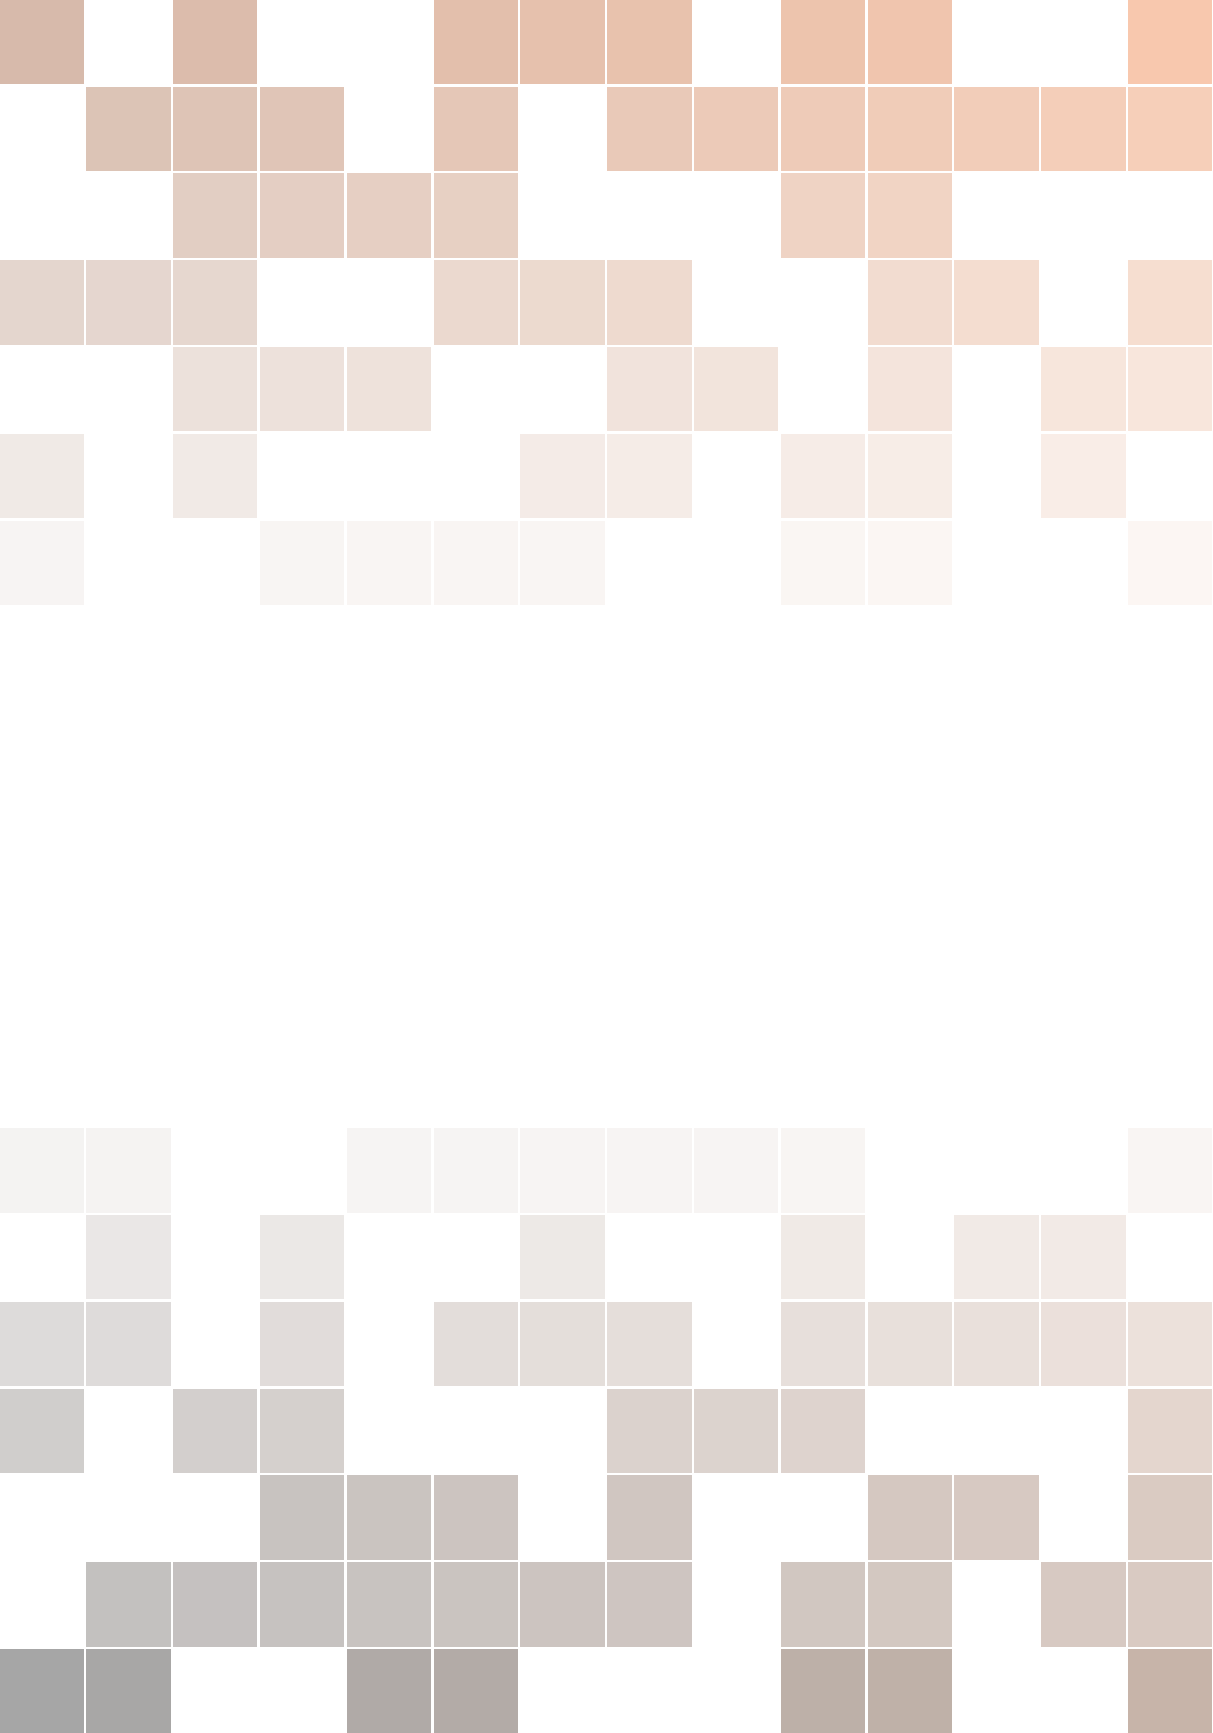
\includegraphics[width=\paperwidth]{background}};
\draw (current page.center) node [fill=ocre!30!white,fill opacity=0.6,text opacity=1,inner sep=1cm]{\Huge\centering\bfseries\sffamily\parbox[c][][t]{\paperwidth}{\centering Complexe Getallen\\[15pt] % Book title
{\Large en hun toepassingen}\\[20pt] % Subtitle
{\huge Karel Dingemanse, Jaap Osseweijer en Siem de Jong}}}; % Author name
\end{tikzpicture}
\vfill
\endgroup

%----------------------------------------------------------------------------------------
%	COPYRIGHT PAGE
%----------------------------------------------------------------------------------------

\newpage
~\vfill
\thispagestyle{empty}

\noindent Copyright \copyright\ 2018 Karel Dingemanse, Jaap Osseweijer en  Siem de Jong\\ % Copyright notice

\noindent \textsc{Gepubliceerd door Griftland College}\\ % Publisher

%\noindent \textsc{book-website.com}\\ % URL

%\noindent Licensed under the Creative Commons Attribution-NonCommercial 3.0 Unported License (the ``License''). You may not use this file except in compliance with the License. You may obtain a copy of the License at \url{http://creativecommons.org/licenses/by-nc/3.0}. Unless required by applicable law or agreed to in writing, software distributed under the License is distributed on an \textsc{``as is'' basis, without warranties or conditions of any kind}, either express or implied. See the License for the specific language governing permissions and limitations under the License.\\ % License information

\noindent \textit{Eerste druk, Februari 2018} % Printing/edition date

%----------------------------------------------------------------------------------------
%	TABLE OF CONTENTS
%----------------------------------------------------------------------------------------

\usechapterimagefalse % If you don't want to include a chapter image, use this to toggle images off - it can be enabled later with \usechapterimagetrue

\chapterimage{chapter_head_1.pdf} % Table of contents heading image

\pagestyle{empty} % No headers

\tableofcontents % Print the table of contents itself

\cleardoublepage % Forces the first chapter to start on an odd page so it's on the right

\pagestyle{fancy} % Print headers again

%----------------------------------------------------------------------------------------
%	PART 1
%----------------------------------------------------------------------------------------

\part{Deel Een}

%----------------------------------------------------------------------------------------
%	CHAPTER 1
%----------------------------------------------------------------------------------------

\chapterimage{chapter_head_2.pdf}

\chapter{Introductie}

Complexe getallen, het zit al in de naam, zijn zeer complex. Wij hebben dit onderwerp gekozen omdat wij wel van complexe uitdagingen houden. Het idee dat er in de wiskunde een imaginair stelsel was riep bij ons veel vragen op, daarom hebben wij dit als onderwerp gekozen.

Na de voorlichtingsdag hadden we een sterk beeld van ons idee en wilde we graag de bèta kant op en dan vooral het vak natuurkunde kiezen. Als tweede keuzen hadden wij het vak wiskunde gekozen omdat dat vak ook binnen onze interesses lag. Wij waren erg benieuwd naar het verloop van het PWS. De samenwerking is altijd al goed geweest tussen ons drieën en onze specialiteiten en interesses sluiten perfect bij elkaar aan.

Wij kregen te horen dat we bij wiskunde waren ingedeeld. Het was even een omschakeling in onze ideeën die we al hadden bedacht voor het vak natuurkunde maar na wat onderzoek en overleg kwamen we op dit fantastisch idee, het complexe getal. Voor ons was het nog een compleet zwart gebied waar we niks van af wisten. Daar wist onze begeleider, meneer Wolterink, wel raad mee. Een pakket wiskunde D over het complexe getal werd ons uitgereikt. Wij zijn met volle moed begonnen aan het raadselachtige imaginaire getal. Na de sommen gemaakt te hebben leek het leuk om er een onderzoek bij te verzinnen en dat was zo makkelijk nog niet, maar onze interesse lag meer bij het gebruik en toepassing van het complexe getal dan echt de theorie er achter. Hebben de toepassingen van complexe getallen raakvlakken?

\section{Hoofdvraag}
Wat is de relatie tussen de verschillende toepassingen van het complex getal? 

\section{Hypothese}
De relatie tussen de verschillende toepassingen van het complex getal is: dat het complex getal gebruikt wordt om gegevens die niet direct te meten of voorspellen zijn te berekenen.

\section{Deelvragen}
Voor de hoofdvraag waren er natuurlijk deelvragen nodig die het complexe getal specifiek uitlegt maar ook op welke gebieden het complexe getal wordt gebruikt en wat nou de relatie tussen die gebieden zijn, met die stellingen zijn wij op deze deelvragen gekomen.

\begin{enumerate}
\item Hoe werken complexe getallen?
\item In welke gebieden worden complexe getallen gebruikt?
\item Wat is de toepassing van complexe getallen bij fractals?
\item Wat is de toepassing van complexe getallen bij Schrödingers vergelijking?
\item Wat is de toepassing van complexe getallen bij signaalverwerking? 
\end{enumerate}

Wij zijn op onderzoek gegaan met een goed, sterk, intelligent en vooral gezellig team.

%----------------------------------------------------------------------------------------
%	CHAPTER 2
%----------------------------------------------------------------------------------------

\chapter{Wat zijn complexe getallen}

\section{De geschiedenis van complexe getallen}

De Italiaanse wiskundigen Scipione del Ferro en Niccolo Fontana Tartaglia kwamen op een nieuw probleem voor het oplossen van de formule van de derdegraads vergelijkingen. Het probleem is namelijk als volgt, wanneer een derdegraads vergelijking wordt opgelost komen er drie oplossingen uit, maar in die drie oplossingen komen ook wortels van negatieve getallen in voor. Dat was nieuw omdat er in die tijd de negatieve getallen nog niet waren gedefinieerd. De naam die de wiskundigen eraan hebben gegeven is daarom ook 'imaginaire getallen', omdat die negatieve getallen er simpel weg dus nog niet waren. Toen de negatieve getallen wel definieert waren werden de normale getallen 'reële getalen' genoemd. Leonhard Euler en Carl Friedrich Gauss legde aan het einde van de 18de de basis voor de getallenleer en de Complexe Functietheorie, hierdoor was het probleem van de Italiaanse wiskundigen opgelost.

De bedenker van de imaginaire getallen is Rafael Bombelli. Hij stelde de rekenregels op voor complexe getallen. Hierbij stelde Rafael als axioma de letter i in zijn boek Algebra (1572).

Een axioma is een niet bewezen maar wel geaccepteerde bewering in de wiskunde en is een belangrijk onderdeel van wiskundige theorieën. Wel is belangrijk dat axioma’s elkaar niet tegenspreken, want dan is de theorie inconsistent. Verder kan een axioma niet uit een andere axioma worden afgeleid, zo’n axioma is dan geen axioma meer maar een bewezen stelling.

Sir William Rowan Hamilton (1805-1865) was de eerste die een formeel correcte opbouw gaf van de complexe getallen met behulp van paren reële getallen (a,b). William is op 4 augustus geboren in het Ierse Dublin en sprak als kleine jongen liefst dertien talen. Zijn interesse is echter verschoven naar de exacte vakken nadat hij op achtjarige leeftijd kennis maakte met het Amerikaanse rekengenie: Zerah Colburn. In 1822 ontdekte William een belangrijke fout in Méchanique céleste van Laplace. Williams is toentertijd benoemd tot beste wiskundige in zijn tijd. In 1833 publiceerde Williams het belangrijke artikel waarin hij complexe getallen als geordende paren reële getallen beschouwde.

De Noorse landmeter Caspar Wessel (1745-1818) was de eerste die complexe getallen voorstelde door middel van punten in het complexe vlak. Ook het gebruik van de poolcoördinaten en vectoren in relatie met complexe getallen is door hem bedacht. Caspar publiceerde in 1799 hierover in een Deens. Omdat Caspar alleen in het Deens publiceerde, is zijn werk aan de aandacht van de 19de-eeuwe wiskundigen ontsnapt. Het complexe vlak is daarna nog twee keer 'ontdekt' door de Fransman Argand in 1806 en door Gauss in 1831. Nadat het werk van Wessel in 1895 opnieuw werd gepubliceerd werd algemeen bekent en aanvaard dat hij de eerste is geweest die de meetkundige voorstelling van complexe getallen heeft bedacht.

\section{Getallenverzamelingen}
In de oudheid, rond 1500 v.C. 'bestonden' alleen de getallen $\{1,2,3,\ldots\}$ Deze getallen dragen de naam natuurlijke getallen \cite{getal_en_ruimte}. Het getal 0 hoort daar sinds 700 v.C. ook bij, want men wilde immers ook kunnen zeggen dat ze naast 4 appels, geen bananen hadden. De berekening
\begin{displaymath}
\text{totale voorraad} = \text{aantal appels}+\text{aantal bananen}=4+0=4
\end{displaymath}
kon nu makkelijk gemaakt worden. Natuurlijke getallen worden aangeduid met $\mathbb{N}$. $\mathbb{N}=\{0,1,2,3,4,5,\ldots\}$.

Op een gegeven moment kwam er een periode waarin ook vergelijkingen als $x + 8 = 5$ opgelost moesten worden. Hiervoor zijn ook negatieve getallen nodig. De verzameling die deze negatieve getallen ook bij zich neemt is de verzameling van de gehele getallen.

Sommige mensen wilden geen hele appels kopen. Nu waren er ook nog breuken nodig. Er komt een verzameling die ook deze breuken erbij neemt. Deze heet de verzameling van de rationele getallen Vergelijkingen als $3x = 7$ konden nu opgelost worden.

Daarnaast was er nog een verzameling van getallen nodig om de vergelijking $x^2 = 7$ op te lossen. De reële getallen. Getallen als $\sqrt{7}$ waren nu acceptabel. Dit was mooi, want nu kon de stelling van Pythagoras worden gebruikt.
\begin{theorem}[Stelling van Pythagoras]\label{eq:pyth}
De stelling van Pythagoras met $c$ als schuine zijde.
\centering{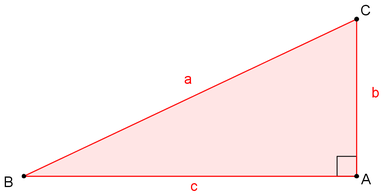
\includegraphics[scale=1]{dh}
\captionof{figure}{Een rechte driehoek.}}
\begin{align}
a^2+b^2=c^2
\end{align}
\end{theorem}
Dit is een formule waarmee zijden van een driehoek met rechte hoek berekend kunnen worden. Bekijk de volgende berekening:
\begin{displaymath}
c=\sqrt{1^2+4^2}=\sqrt{17}.
\end{displaymath}

Tot de verzameling van de reële getallen behoren ook de irrationele getallen zoals $\pi$, $\sqrt{2}$ en $\sin{(10)}$. Dit zijn getallen die niet te schrijven zijn als het quotiënt\footnote{Quotiënt betekent: het resultaat van een deling.} van twee gehele getallen.

In de Fig. \ref{fig:verzameling} is weergegeven wat de relaties tussen de verschillende getallenverzamelingen zijn.

\begin{figure}[h]
	\centering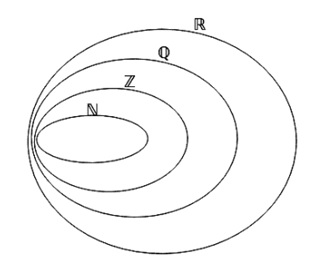
\includegraphics[scale=1]{verzameling}
	\caption{Verschillende getallenverzamelingen.}
	\label{fig:verzameling}
\end{figure}

\begin{definition}[Reële getallenverzamelingen]\label{eq:rf}
Dit zijn de reële getallenverzamelingen.
\begin{align}
\mathbb{N} \subset \mathbb{Z} \subset \mathbb{Q} \subset\mathbb{R}\footnotemark
\end{align}
\footnotetext{A $\subset$ B betekent: ieder element van A is ook een element van B. Ofwel, A is een subset van B.}
\end{definition}

Los je de vergelijking $x^3-5x=0$ op in $\mathbb{Q}$, dan krijg je
\begin{displaymath}
\begin{aligned}
x^3-5x&=0\\
x(x^2-5)&=0\\
x=0 \quad &\vee \quad x^2=5\\
x=0 \quad &\vee \quad \text{geen oplossing in } \mathbb{Q}
\end{aligned}
\end{displaymath}
Er zijn naast $x=0$ geen oplossingen in $\mathbb{Q}$, want $\sqrt{5}$ is geen rationeel getal.

Maar zoals al aangegeven was, is er meer! Om $x^2=-1$ op te lossen kan je niet gebruik maken van $\mathbb{R}$. De wiskundige Euler was de eerste die het getal waarvan het kwadraat -1 is gebruikte in rekensommetjes. De letter $i$ (die je vanaf nu veel gaat zien) komt van 'imaginary' wat imaginair betekent.
\begin{definition}[Imaginair getal]
Voor het imaginaire getal geldt dat
\begin{align}
i^2  = -1
\end{align}
\end{definition}
Dit is vreemd, want eerst was het kwadraat van een getal in ieder geval positief volgens de regel min maal min is plus. Ofwel, $(-1)^2=1$ is gelijk aan $-1\cdot-1=1$.

De vergelijking $x^2 = -1$ is als volgt op te lossen.
\begin{displaymath}
\begin{aligned}
x^2 &= -1\\
x^2 &= i^2\\
x=i \quad &\vee \quad x=-i
\end{aligned}
\end{displaymath}
Hierin is te zien dat een imaginair getal een getal is in de vorm $bi$, met $b \in R$\footnote{$A \in B$ betekent: element A is onderdeel van de verzameling B} . Dus in bovenstaande berekening geldt dat
\begin{displaymath}
b=1 \quad \vee \quad b=-1.
\end{displaymath}

Zo ook
\begin{displaymath}
\begin{aligned}
x^2 &= -4\\
x=2i \quad &\vee\quad  x=-2i.
\end{aligned}
\end{displaymath}
Dus in dit geval is
\begin{displaymath}
b = 2 \quad  \vee \quad b = -2
\end{displaymath}

Er zijn dus ook imaginaire getallen. Dit zijn getallen die alleen uit het product van een reëel getal en $\sqrt{-1}$ bestaan. Imaginaire getallen worden aangeduid met het symbool $\mathbb{I}$.

Dan heb je ook nog de verzameling van de complexe getallen. Dat zijn getallen die uit een reëel en een imaginair deel bestaan, zoals
\begin{displaymath}
a + bi.
\end{displaymath}
Het symbool die de verzameling van complexe getallen weergeeft is $\mathbb{C}$. Van een complex getal $a + bi$ wordt $a$ het reële deel en $b$ het imaginaire deel genoemd.

\begin{definition}[Reële en complexe getallenverzamelingen]
De getallenverzamelingen van de reële en complexe getallen.
\begin{align}
\mathbb{N} \subset \mathbb{Z} \subset \mathbb{Q} \subset\mathbb{R} \subset \mathbb{C}
\end{align}
\end{definition}

\begin{figure}[h]
	\centering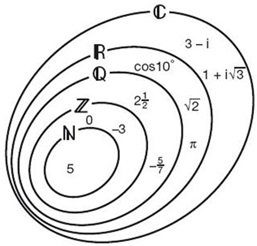
\includegraphics[scale=1]{verzameling2}
	\caption{Reële en complexe getallenverzamelingen.}
	\label{fig:verzameling2}
\end{figure}

\section{De basis}
In deze sectie bespreken we hoe je werkt met complexe getallen.
\subsection{Rekenregels}
De rekenregels voor complexe getallen mogen de rekenregels van reële getallen niet tegen spreken, want de getallenverzameling $\mathbb{R}$ is onderdeel van de getallenverzameling $\mathbb{C}$. Wat voor $\mathbb{R}$ werkt moet dus ook voor $\mathbb{C}$ werken. Voor de simpele berekeningen met complexe getallen (sommen met optellen, aftrekken, vermenigvuldigen en delen) zijn er simpele rekenregels.
\begin{alignat*}{5}
\text{optellen}& \qquad &&(a+bi) &&+ &&(c+di) &&=(a+c)+(b+d)i\\
\text{aftrekken}& \qquad &&(a+bi) &&- &&(c+di) &&=(a-c)+(b-d)i\\
\text{vermenigvuldigen}& \qquad &&(a+bi) &&\cdot &&(c+di) &&=(ac-bd)+(ad+bc)i\\
\text{delen}& \qquad &&(a+bi) &&: &&(c+di) &&=((ac+bd)+(ad-bc)i):(c^2+d^2)
\end{alignat*}

Als we dan het complexe getal $z = a + bi$ hebben, kunnen hier ook het geconjugeerde van nemen.
\begin{displaymath}
\conj{z}=\conj{a+bi}=a-bi
\end{displaymath}

De letterlijke betekenis van geconjugeerde is: gekoppeld of samengaand. In de wiskunde is een complex geconjugeerde (ook wel een complexe toegevoegde genoemd) van een complex getal hetzelfde imaginaire of complexe getal met hetzelfde reële deel, maar dan met een tegengesteld of negatief imaginaire gedeelte. Alsof de imaginaire functie voor een spiegel staat en alles in spiegelbeeld nadoet. Dus als een complex getal in een complex vlak wordt weergegeven is het geconjugeerde het om de reële as gespiegelde getal. Als het complexe getal en het complex geconjugeerde met elkaar vermenigvuldigd wordt komt er een reëel getal uit, zie Fig. \ref{fig:geconjugeerd}.

\begin{figure}[h]
	\centering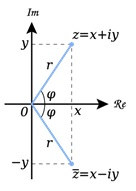
\includegraphics[scale=1]{geconjugeerd}
	\caption{De geconjugeerde in het complexe vlak.}
	\label{fig:geconjugeerd}
\end{figure}

En hieruit kunnen we weer de volgende regel opstellen.
\begin{displaymath}
(a+bi)\cdot(\conj{a+bi})=a^2+b^2
\end{displaymath}
want
\begin{displaymath}
\begin{aligned}
(a+bi)\cdot(\conj{a+bi}) &= (a+bi)\cdot(a-bi)\\
&= (a^2--b^2)+(-ab+ab)i\\
&= a^2+b^2.
\end{aligned}
\end{displaymath}

\subsection{Het complexe vlak}
Omdat het imaginaire deel i van complexe getallen uit $\mathbb{C}$ niet is uit te drukken in $\mathbb{R}$, heeft deze dus ook geen plaats op de getallenlijn van $\mathbb{R}$ en is deze dus ook niet uit te beelden in een reëel assenstelsel. Daarom is er voor de getallen verzameling $\mathbb{C}$ een nieuw assenstelsel gecreëerd: het complexe vlak. Deze wordt ook wel het vlak van Gaus of een arganddiagram genoemd. Dit vlak lijkt qua uiterlijk zeer op een reëel assenstelsel, maar in plaats van een x-as heb je een reële as, waar het reële deel van een complex getal wordt aangegeven en in plaats van de y-as het een imaginaire as, waar het imaginaire deel van een complex getal wordt aan gegeven. Op de horizontale as dus het reële deel en op de verticale as dus het imaginaire deel.

Een punt aangeven in het complexe vlak is goed te doen wanneer het complex getal is uitgedrukt als $z = a + bi$, waar a de positie op reële as aangeeft en bi de positie op de imaginaire as aangeeft. Complexe getallen in het complexe vlak bij elkaar optellen is dan ook goed te doen volgens de eerdergenoemde rekenregels.

Neem de optelling. Geschreven in coördinaten zou hier het volgende staan.
\begin{displaymath}
(a,b)+(c,d)=(a+c,b+d)
\end{displaymath}

Weergeven in het complexe vlak kan dit ook worden gedaan volgens de parallellogramconstructie.

De lengte van $z = a + bi$ in het complexe vlak kan worden berekend door middel van de Stelling van Pythagoras (Vgl. \ref{eq:pyth}), waar de lengte gelijk is aan $\sqrt{a^2+b^2}$. Deze lengte wordt de modulus of absolute waarde van $z = a + bi$ genoemd en wordt als volgt genoteerd.
\begin{displaymath}
|z|=|a+bi|=\sqrt{a^2+b^2}
\end{displaymath}

Hieruit kunnen we nog enkele andere rekenregels en stellingen afleiden.
\begin{theorem}[Absolute waarde complexe getallen]
De absolute waarde van een complex getal kan als volgt berekend worden.
\begin{align}\label{eq:abs}
\left|z\right|=\sqrt{{\Re (z)}^2+{\Im (z)}^2}=\sqrt{z\conj{z}}\footnotemark
\end{align}
\footnotetext{$\Re$ en $\Im$ staan respectievelijk voor het reële en het imaginaire gedeelte van een complex getal.}
\text{en zo ook}
\begin{align}\label{eq:abs2}
|z_1\cdot z_2|=|z_1|\cdot |z_2|\quad\text{met } z_1=a+bi \quad\text{ en } z_2=c+di
\end{align}
\end{theorem}

Vgl. \ref{eq:abs2} klopt, want
\begin{align*}
|z_1\cdot z_2 |&=|(a+bi)\cdot(c+di)|\\&=|(ac-bd)+(ad+bc)i|\\&=\sqrt{(ac-bd)^2+(ad+bc)^2)}\\&=\sqrt{(a^2 c^2-2abcd+b^2 d^2+b^2 c^2+2abcd+a^2d^2)}\\&=\sqrt{(a^2 c^2+a^2 d^2+b^2 c^2+b^2d^2)}
\end{align*}
\begin{align*}
|z_1 |\cdot|z_2 |&=|a+bi|\cdot|c+di|\\&=\sqrt{(a^2+b^2 )}\cdot\sqrt{(c^2+d^2 )}\\&=\sqrt{(a^2+b^2 )\cdot(c^2+d^2 )}\\&=\sqrt{(a^2 c^2+a^2 d^2+b^2 c^2+b^2d^2)}
\end{align*}

\begin{figure}[h]
	\centering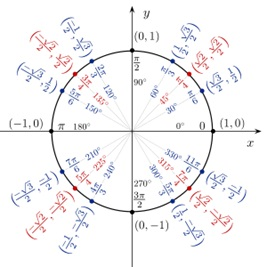
\includegraphics[scale=1]{ehc}
	\caption{De eenheidscirkel.}
	\label{fig:ehc}
\end{figure}

Zo meteen wordt besproken hoe je de 'draaiingshoek' van een complex getal kan bepalen. Hiervoor moet je eerst weten hoe je dat met reële getallen doet. Daarvoor moet je eerst weer wat over de eenheidscirkel weten. De eenheidscirkel is een cirkel in het reële vlak met de oorsprong, het punt $O(0,0)$, als middelpunt en een straal, de lengte van het middelpunt tot lijn van de cirkel, van 1.

\begin{definition}[Omtrek van een cirkel]
De omtrek van een cirkel is als volgt uit te rekenen.
\begin{align}\label{eq:2pir}
2\pi r=\pi d \quad\text{waar } r \text{ de straal is en } d \text{ de diameter}
\end{align}
\end{definition}

De straal in de eenheidscirkel is $1$, dus de omtrek is $2\pi$. Al aangegeven in Fig. \ref{fig:ehc}, geldt dat de $x$-coördinaat gelijk staat aan $\cos{(t)}$ en de $y$-coördinaat gelijk staat aan $\sin{(t)}$, met $t$ als draaiingshoek.

Om te weten wat de draaiingshoek van het punt $P(\frac{1}{2}\sqrt{3},\frac{1}{2})$ is, maakt men de volgende berekening.
\begin{align*}
\cos{(t)}&=\frac{1}{2}\sqrt{3}\\
t&=\frac{1}{6}\pi+k\cdot 2\pi
\end{align*}
Waarom '$+ k\cdot2\pi$'? Dit omdat na iedere keer dat je $2\pi$ toevoegt aan je draaiingshoek, je weer op hetzelfde punt uitkomt, maar dan een rondje verder, want zoals eerder gezegd is de omtrek van de cirkel $2\pi$.

Om de draaiingshoek (aangegeven met $\phi$, de Griekse letter phi) van een complex getal $z$ in het complexe vlak te weten te komen moet je het argument van $z$ berekenen.
\begin{definition}
Het argument van een complex getal is als volgt te berekenen.
\begin{alignat*}{2}
\phi &=\text{arg}(z)\quad &\text{ mits }z\neq 0\\
\phi &= \arctan\left(\frac{b}{a}\right)\quad &\text{met } b=\Im(z) \text{ en } a=\Re(z)
\end{alignat*}
\end{definition}
Dit geeft echter vaak onhandige antwoorden, dus het is beter om de arg functie (in je Casio-rekenmachine) of de Angle functie (als je een TI-rekenmachine hebt) te gebruiken. Hieruit volgt een argument in radialen, dit is vermenigvuldiging van $\pi$, maar ook het berekende argument $+$/$-$ $2\pi$.
\begin{align*}
\phi&=\text{arg}(z)\qquad\text{met } z=1+i\\
&=\frac{1}{4}\pi + k\cdot 2\pi\\
\end{align*}

Het argument van $z$ dat tussen $\pi$ en $-\pi$ ligt wordt ook wel hoofdargument genoemd en wordt dat geschreven als $\text{Arg}(z)$. Van het hierboven gegeven voorbeeld geldt dus $\text{Arg}(z)=\frac{1}{4} \pi$.

\subsection{Poolcoördinaten}
In het reële assenstelsel worden punten aangegeven met cartesische coördinaten, ofwel de $x$- en $y$-coördinaten van een punt. In het complexe vlak is deze manier van punt aanduiding eigenlijk niet bruikbaar, want er is in het complexe vlak geen sprake van een $x$- of $y$-as. In plaats daarvan wordt bij een punt in het complexe vlak de modulus van het punt tot de oorsprong en draaiingshoek van het punt gebruikt. Dit zijn de poolcoördinaten van het punt. De poolcoördinaten zijn simpel weg een andere manier van coördinaten aanduiden zonder het gebruikt van een $x$- of $y$-coördinaat en poolcoördinaten kunnen ook gebruikt worden in het reële assenstelsel. Voor het gemak geven we daarom ook een eerste voorbeeld van het gebruik van poolcoördinaten in het reële assenstelsel (Fig. \ref{fig:pool}).

\begin{figure}[h]
	\centering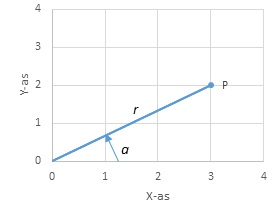
\includegraphics[scale=1]{pool}
	\caption{Poolcoördinaten reëel assenstelsel.}
	\label{fig:pool}
\end{figure}

Voor de poolcoördinaten van punt P hebben we de modulus $r$ en de draaiingshoek $a$ nodig.
\begin{align*}
r=OP&=\sqrt{x_p^2+y_p^2}\\
&=\sqrt{3^2+2^2}\\
&=\sqrt{9+4}\\
&=\sqrt{13}
\end{align*}
\begin{align*}
\tan{(a)}&=\frac{2}{3}\\
a&=\arctan{\left(\frac{2}{3}\right)}\\
&\approx 0,588
\end{align*}
De poolcoördinaten van P noteer je dan als P$(\sqrt{13};0,588)$. De draaiinghoek van poolcoördinaten wordt aangegeven met $\theta$ (de Griekse letter thèta) en de draaiingshoek moet tussen $\pi$ en $-\pi$ liggen. Bekijk de drie basisverhoudingen van de goniometrie.
\begin{definition}
De basisverhoudingen van de goniometrie.
%\begin{figure}[h]
%	\centering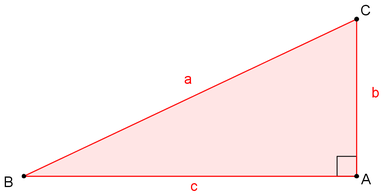
\includegraphics[scale=1]{dh}
%	\caption{Een rechte driehoek.}
%	\label{fig:dh}
%\end{figure}
\begin{alignat}{3}
\sin{B} &=\frac{\left|AC\right|}{\left|BC\right|} &=\frac{b}{a} &=\frac{\text{overstaande rechthoekszijde}}{schuinezijde}\\
\cos{B} &=\frac{\left|AB\right|}{\left|BC\right|} &=\frac{c}{a} &=\frac{\text{aanliggende rechthoekszijde}}{schuinezijde}\\
\tan{B} &=\frac{\left|AC\right|}{\left|AB\right|} &=\frac{b}{c} &=\frac{\text{overstaande rechthoekszijde}}{aanliggende rechthoekszijde} \label{eq:tan}
\end{alignat}
\end{definition}
\begin{theorem}\label{th:a}
Nu we Vgl. \ref{eq:abs} op pagina \pageref{eq:abs} en \ref{eq:tan} hebben gezien, kunnen we het volgende zeggen.
\begin{align}
x &= r\cos{(\theta)}\\
y &= r\sin{(\theta)}
\end{align}
\end{theorem}
Met Stelling \ref{th:a} kunnen we poolcoördinaten omrekenen naar cartesische coördinaten en andersom.

Het complexe getal kun je ook noteren met behulp van poolcoördinaten.
\begin{align*}
r &=\left|z\right|,\\
\theta &=\phi=\text{arg}(z),\\
\Re(z) &=\left|z\right|\cos{(\phi)},\\
\Im(z) &=\left|z\right|\sin{(\phi)}.
\end{align*}
\begin{align*}
z &=\left|z\right|\cos{(\phi)}+i\left|z|\right|\sin{(\phi)}\\
&= r\cos{(\phi)}+ir\sin{(\phi)}\\
&= r(\cos{(\phi)}+i\sin{(\phi)}
\end{align*}

\subsection{Formule van Euler}
Een zeer bekende formule die met complexe getallen verwant staat, is de formule van Euler.
\begin{equation}\label{eq:euler}
e^{i\phi}=\cos{(\phi)}+i\sin{(\phi)}\footnotemark
\end{equation}\footnotetext{met $e \approx 2,718281828459\ldots$}
Om te begrijpen waar deze formule vandaan komt, moet men eerst begrijpen wat een afgeleide (of differentiaalvergelijking) is. Dit is namelijk een onderdeel van het bewijs waarmee aangetoond wordt dat bovenstaande formule klopt.

Zoals men weet, bestaat een grafiek uit een functie zoals
\begin{displaymath}
f(x)=-3x^2-2x+20.
\end{displaymath}
Deze grafiek is een parabool en ziet eruit als in Fig. \ref{fig:fx3}.
\begin{figure}[h]
	\centering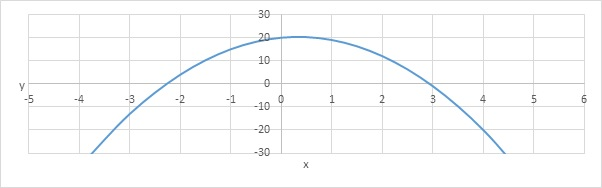
\includegraphics[scale=1]{fx}
	\caption{De grafiek $f(x)=-3x^2-2x+20$, geplot.}
	\label{fig:fx3}
\end{figure}
Als we van van deze grafiek de top willen hebben we de afgeleide van de functie nodig.
\begin{definition}
De afgeleide wordt aangegeven met een apostrof na de functienaam en een vorm wordt als volgt berekend.
\begin{align}
f(x)=x^n
f'(x)=n\cdot x^{n-1}
\end{align}
\end{definition}
Bij de eerder gebruikte functie kunnen we dan de afgeleide berekenen.
\begin{align*}
f(x) &=-3x^2-2x^1+20\\
&=-3x^2-2x^1+20x^0\\
f'(x) &= 2\cdot -3x^{2-1}+1\cdot 2x^{1-1}+0\cdot 20x^{0-1}\\
&=-6x^1+2x^0 +0x^{-1}\\
&=-6x+2
\end{align*}
Deze afgeleide wordt in Fig. \ref{fig:f'x} in oranje weergegeven.
\begin{figure}[h]
	\centering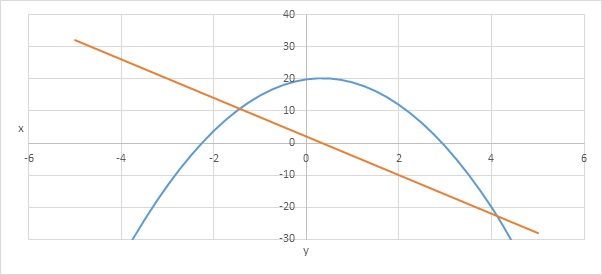
\includegraphics[scale=1]{f'x}
	\caption{De grafiek $f(x)=-3x^2-2x+20$ en zijn afgeleide, geplot.}
	\label{fig:f'x}
\end{figure}

Dit is dus een rechte lijn in plaats van een parabool. Je kan zien dat de afgeleide de helling van de grafiek in alle punten aangeeft. Als we dan de afgeleide gelijkstellen aan 0 hebben we het x-coördinaat van de top van de grafiek, wetende dat de richting van de lijn in de top 0 is.
\begin{align*}
f'(x) &= 0\\
x &= \frac{1}{3}
\end{align*}

Een speciaal getal bij de differentiëren is het getal $e$. Wat speciaal is aan $e$ is het feit dan de afgeleide van $e^x$ nog steeds $e^x$ is.
\begin{definition}
De afgeleide van een e-macht.
\begin{align}
f(x)=e^x
f'(x)=e^x
\end{align}
\end{definition}

Wetende dat de afgeleide van $e^x$ nog steeds $e^x$ is, kunnen we met dit feit van ex een som van oneindige $x$ machten schrijven. Deze machtreeks schrijven we dan als volgt.
\begin{align*}
f(x)=e^x=a_0+a_1x+a_2x^2+a_3x^3+\ldots
\end{align*}
Hiervan is de afgeleide het volgende.
\begin{align*}
f'(x)=e^x=a_1+2a_2x+3a_3x^2+4a_4x^3+\ldots
\end{align*}
De tweede afgeleide wordt nu.
\begin{align*}
f''(x)=e^x=2a_2+6a_3x+12a_4x^2+20a_5x^3+\ldots
\end{align*}

Op $x=0$, $f(0)=e^0=1$. Daarbij is $a_0=1$, want alle $a\cdot x^n=0$. Bij $f'(0)$, $a_1=1$. Bij $f''(0)$, $2a_2=1$. Bij $f'''(0)$, $6a_3=1$, etc. Dit geeft het volgende.
\begin{align*}
a_2 &=\frac{1}{2}=\frac{1}{2!}\\
a_3 &=\frac{1}{6}=\frac{1}{3!}
\end{align*}
We kunnen hieruit het volgende concluderen.
\begin{align*}
a_n=\frac{1}{n!}
\end{align*}

Hier zie je achter een natuurlijk getal een $!$ Staan. Daar wordt de faculteit mee bedoelt, die wordt genoteerd als $n!$. Een faculteit is een product van een getallen $1$ tot en met $n$. Een voorbeeld hiervan is $5!$, dan is $1*2*3*4*5= 120$. De waardes van een faculteit groeien enorm snel en wordt veel gebruikt bij rangschikkingen of combinaties van verschillende soorten getallen.

Als we dit concept van machtreeksen toepassen op sinussen en cosinussen krijgen we het volgende.
\begin{align*}
f(x) &=\sin{(x)} &=a_0+a_1x+a_2x^2+a_3x^3+\ldots\\
f(0) &=\sin{(0)} &=0
\end{align*}
Dus $a_0=0$.

Wetende dat $\left[\sin(x)\right]'=\cos(x)$ en $\left[\cos(x)\right]'=-\sin(x)$ kunnen we het volgende zeggen.
\begin{align*}
f'(x) &= \cos(x) = a_1+2a_2x+3a_3x^2+4a_4x^3+\ldots\\
f'(0) &= \cos(0) = 1
\end{align*}
dus $a_1=1$.
\begin{align*}
f''(0) =-\sin(0) = 0
\end{align*}
Dus $2a_2=0$.
\begin{align*}
f'''(0) =-\cos(0) = -1
\end{align*}
Dus $6a_3=1$
\begin{align*}
f''''(0) =\sin(0) = 0
\end{align*}
Dus $24a_4=0$.

Hieruit kunnen we afleiden dat bij $\sin(x)$ alle even $a$’s $\{a_0, a_2, a_4, a_6, \ldots\}$ gelijk zijn aan $0$ en dat bij $\cos(x)$ alle oneven $a$’s $\{a_1, a_3, a_5, \dots\}$ gelijk zijn aan 0. Zo kunnen we het volgende opstellen.
\begin{align*}
\sin(x) &=x-\frac{x^3}{3!}+\frac{x^5}{5!}-\frac{x^7}{7!}+\ldots
\cos(x) &= 1-\frac{x^2}{2!}+\frac{x^4}{4!}-\frac{x^6}{6!}+\ldots
\end{align*}
Als dan het imaginair getal in mix gooien door in plaats van $e^x$ juist $e^{ix}$ te nemen wordt de machtenreeks als volgt.
\begin{align*}
e^{ix} &=1+x\cdot i+\frac{x^2}{2!}i^2+\frac{x^3}{3!}i^3+\frac{x^4}{4!}i^4+\frac{x^5}{5!}i^5+\ldots
&= 1+x\dots i +\frac{x^2}{2!}\cdot -1+\frac{x^3}{3!}-i+\frac{x^4}{4!}\cdot 1+\frac{x^5}{5!}\cdot i+\ldots
&= 1+xi-\frac{x^2}{2!}-\frac{x^3}{3!}i+\frac{x^4}{4!}+\frac{x^5}{5!}i-\frac{x^6}{6!}-\frac{x^7}{7!}i+\ldots
\end{align*}
Dit kan je verder verkleinen tot Vgl. \ref{eq:euler} op pagina \pageref{eq:euler}.

Als we deze vergelijken met de manier van het complexe getal schrijven die is gevonden bij de poolcoördinaten: $z = r\cos(\phi) + i\sin(\phi)$, kunnen we de formule van Euler herkennen. Zo kunnen we het complexe getal dus ook schrijven als $z = r\cdot e^{i\phi}$ met $r=\left|z\right|$ en $\phi=\text{arg}(z)$.

\subsection{Complexe e-machten}
Voor de complexe e-machten gelden dezelfde rekenregels als voor reële e-machten.
\begin{align*}
ae^c\cdot be^d=(a\cdot b)e^{c+d}\qquad \frac{ae^c}{be^d}=\frac{a}{b}e^{c-d}\qquad (ae^c)^d=a^de^{c\cdot d}
\end{align*}
Met complexe e-machten wordt het dan het volgende.
\begin{align*}
ae^ci\cdot be^di=(a\cdot b)e^{(c+d)i}\qquad \frac{ae^ci}{be^di}=\frac{a}{b}e^{(c-d)i}\qquad (ae^{ci})^d=a^de^{(c\cdot d)i}
\end{align*}

\subsection{Complexe wortels}
Bekijk de berekening.
\begin{align*}
z &= \sqrt{3}+i\\
z^3 &= (\sqrt{3}+i)^3\\
&= (3+2i\sqrt{3}+i^2)(\sqrt{3}+i)\\
&= 3\sqrt{3}+6i+i^2\sqrt{3}+3i+2i^2\sqrt{3}+i^3\\
&= 3\sqrt{3}-\sqrt{3}-2\sqrt{3}+6i+3i-i\\
&= 8i\\
&= -8\cdot -i\\
&= (-2)^3\cdot i^3\\
&= (-2i)^3\\
z &= (-2i)
\end{align*}

We zien dat $z^3=8i$ drie oplossingen heeft, maar als we $-2i$ schrijven als $re^{i\phi}$ kunnen we dat ook op meerdere manieren doen.
\begin{align*}
z=-2i=2e^{-\frac{1}{2}\pi i+k\cdot 2\pi i}
\end{align*}
De $k\cdot 2\pi i$ is de complexe vorm van $k\cdot 2\pi$ en betekend dat we een rondje over de complexe eenheidscirkel lopen. Dan kunnen we zo het volgende berekenen.
\begin{alignat*}{2}
z^3 &=8i &\\
z^3 &=8e^{\frac{1}{2}\pi i +k\cdot 2\pi i} &\\
z &={(8e^{\frac{1}{2}\pi i +k\cdot 2\pi i})}^{\frac{1}{3}} &\\
&= 2e^{\frac{1}{6}\pi i+k\cdot \frac{2}{3}\pi i} &\\
z &=\sqrt{3}+i\quad &\text{met }k=0 \\
\vee \; z &=-\sqrt{3}+i\quad &\text{met }k=1\\
\vee \; z &=-2i\quad &\text{met }k=2
\end{alignat*}

\subsection{Draaisymmetrie}
De drie oplossingen van $z^3=8i$ hebben een absolute waarde van $2$ en liggen dus op de cirkel met het middelpunt $0$ en een staal van $2$ getekend in het complexe vlak. De argumenten van de oplossingen verschillen steeds $\frac{2}{3}\pi$. Als je dan dus één van de oplossingen hebt gevonden kun je de rest van de oplossingen vinden door middel van draaisymmetrie ofwel door $\frac{2}{3}\pi$ bij het gevonden argument op te tellen. De drie oplossingen van $z^3=8i$ noteren we als $\sqrt[3]{8i}$, hiermee wordt dus $\sqrt{3}+i$, $-\sqrt{3}+i$ en $-2i$ bedoelt.
Zo is de complexe wortel $\sqrt{4i}$ tweewaardig (heeft twee oplossingen) en is de complexe wortel $\sqrt[3]{8i}$ driewaardig (heeft drie oplossingen). Zo zijn alle complexe wortels meerwaardig. Dus:
Bij $z^n=c$ met $\{n=2, 3, 4, \ldots\}$ en $c\neq 0$ heeft $z$ precies $n$ aantal oplossingen in $\mathbb{C}$
Deze oplossingen kun je vinden door één oplossing te bereken met $z^n=re^{i\phi+k*2\pi i}$ en de rest van de oplossingen te vinden door middel van draaisymmetrie: $\text{arg}+\frac{2\pi}{n}$.

%----------------------------------------------------------------------------------------
%	CHAPTER 3
%----------------------------------------------------------------------------------------

\chapter{Toepassingsgebieden van complexe getallen}
De oorspronkelijke reden dan de complexe getallen verzameling en het imaginair getal in het leven werd geroepen, was om een derdegraads vergelijking op te lossen. Want toen de Italiaanse wiskundigen Scipione del Ferro en Noccolo Fontana Tartaglia in de zestiende eeuw, gepaard met een hevig conflict, met een formule voor het oplossen van een derdegraads vergelijking kwamen, raakte de wiskundige wereld van die tijd in rep en roer. Bij de berekeningen die de Italianen gebruikte namen ze namelijk wortels uit negatieve getallen, wat in de reële wiskunde simpelweg niet kan. Of in ieder geval niet in die tijd. Men had toen geen idee hoe ze wortels uit negatieve getallen moesten definiëren. En omdat ze dus geen idee hadden hoe ze die getallen moesten omschrijven, is het ook niet ver gezocht dat ze naar die getallen zijn gaan refereren als imaginaire (denkbeeldige) getallen.
Dit was lange tijd dus een onoplosbaar probleem in de wiskunde, totdat Leonhard Euler en Carl Friedrich Gauss in de achttiende eeuw de wiskunde voorgoed veranderde door dus de complexe getallen verzameling te introduceren. Hiermee konden ze dus eindelijk een 'logische' oplossing geven voor de wortel van een negatief getal en zo dus een derdegraads wortel oplossen. 
Maar later werd al snel duidelijk dat deze nieuwe getallenverzameling kon worden gebruikt om veel meer problemen in zowel de wiskunde, als in andere wetenschappelijke vlakken als natuurkunde en economie op te lossen en zo antwoorden te krijgen op eerst onmogelijk lijkende vragen. Deze andere problemen en oplossingen in de andere vlakken gaan we dus ook verder bespreken in dit hoofdstuk.

De complexe getallen, vormen een uitbreiding van de verzameling der reële getallen. Zoals de reële getallen worden voorgesteld als punten op de getallenrechte, zo kunnen de complexe getallen worden voorgesteld als punten in het platte vlak. Complexe getallen spelen niet zo’n zichtbare rol in het dagelijkse leven zoals de gehele getallen en de breuken en hebben, onder meer om die reden, een zekere mysterieuze status. Ze spelen des te meer een rol in wetenschapsgebieden zoals economie, biologie, natuurkunde, scheikunde, elektrotechniek en wiskunde. Via die wetenschapsgebieden bepalen ze natuurlijk mede de inrichting van onze maatschappij. Wij bespreken enkele voorbeelden van deze vakgebieden waar complexe getallen een rol spelen:

\section{Natuurkunde}
In de klassieke natuurkunde werden complexe getallen gebruikt voor het bijhouden van de twee coördinaten van tweedimensionale vectoren. Deze complexe getallen bevatten ook informatie over de lengte van de vectoren. Op deze manier complexe getallen gebruiken was niet echt fundamenteel voor de natuurkunde. Zeker niet het vermenigvuldigen van complexe getallen.
Dit veranderde toen kwantummechanica een ding werd. De golven in kwantummechanica houdt zich bezig met een van de kleinste deeltjes die men zich kan voorstellen. De golven binnen de kwantummechanica moesten worden voorgesteld door $e^ikx$ \cite{motl} als het moment en de richting van de beweging moesten worden gebruikt. In de kwantummechanica bestaat een van de stappen zo goed als altijd uit het kwadrateren van absolute waarden van complexe waarschijnlijkhedenamplitudes.
Een ander zeer groot toepassingsgebied is elektrotechniek. Daar hebben ze veel te maken met sinusoïden. Engineers zijn lui. In plaats van dat ze een golfbeweging duidelijk beschrijven met evenwichtsstand, amplitude, vermenigvuldiging t.o.v. $x$- en $y$-as en fase kunnen ook zij nu een sinusoïde beschrijven in de vorm $e^{it}$ \cite{harish}. Het werkt makkelijk, want is makkelijker op te schrijven en het is makkelijker om ermee te rekenen. Twee sinusoïden vermenigvuldigen gaat met deze vorm veel makkelijker dan een klassieke representatie.
Het blijft niet bij kwantum en elektro. Complexe getallen worden ook reeds gebruikt bij bijvoorbeeld vloeistofdynamica, signaalanalyse, meet- en regeltechniek, differentiaalrekeningen en relativiteit \cite{complex_numbers}.

\section{Econometrie}
In het vakgebied van de econometrie wordt er hier en daar ook gebruik gemaakt van complexe getallen. Bij de econometrie wordt er naar wiskundige vergelijkingen gezocht die verschijnselen in de wereld verklaren. Er wordt extreem veel data verzameld en in die data wordt naar dingen gezocht die invloed op elkaar hebben. Als er dan eenmaal een verband wordt gevonden gaan econometristen aan de slag om een wiskundig model te maken die dit soort verschijnselen in de toekomst kunnen verklaren. En als de econometristen hun werk goed hebben gedaan kunnen ze dat model ook gebruiken om vergelijkbare omstandigheden in de toekomst te voorspellen
Zo gaat een econometrist opzoek naar een wiskundig stelsel die de meest efficiënte manier om pakketjes te bezorgen kan berekenen. Als het model goed werkt is het niet alleen toepasbaar op een kleine schaal, zoals een wijk of een klein dorp, maar werkt het ook op een grotere schaal, zoals een grote stad of misschien zelfs een groter gebied. Het onderwerp van het model hoeft niet perse economisch te zijn, zo werden econometristen ingeschakeld om de grote van de olievlek na het lek in de Golf van Mexico te voorspellen
Om de modellen zo precies mogelijk te maken is het soms nodig voor de econometristen om complexe getallen te gebruiken. Het gebeurt echter niet vaak dat complexe getallen worden gebruikt in de voorspellingen. Een voorbeeld van modellen of berekeningen waar complexe getallen worden gebruikt is de tijdsbepaling van een bepaalde hoogte van een getij. Er zijn dan modellen ontwikkeld die gebruik maken van complexe getallen waarmee je zeer nauwkeurig kunt berekenen wanneer het water een bepaalde hoogte gaat hebben en of het water dan gaat dalen of stijgen. Verder worden complexe getallen bijvoorbeeld gebruikt om analyses van wachtrijsystemen te maken. Zo wordt het makkelijker om de verwachte wachtrijlengte en -tijd zo exact mogelijk te bepalen om het op die manier in de praktijk alles soepeler te laten verlopen.

\section{Wiskunde}
In de wiskunde kom je de basis tegen van het complexe getal. Zonder de hedendaagse wiskunde kan er geen complex getal bestaan. Het complexe getal kan overal worden toegepast in de wiskunde maar is voor sommige aspecten van de wiskunde cruciaal. 
Een belangrijke toepassing van complexe getallen kom je tegen bij het oplossen van differentiaalvergelijkingen \cite{dg}. Bij het oplossen van een differentiaalvergelijking zoek je naar alle mogelijke oplossingen van deze differentiaalvergelijking. Deze oplossingen verschillen slechts in een of meerdere constanten van elkaar. Een oplossing waarin nog onbekende constanten voorkomen, noemt men een algemene oplossing van de differentiaalvergelijking. Zijn de waarden van deze constanten bekend, dan spreekt men van een specifieke oplossing. Veel technische en natuurkundige verschijnselen kunnen worden beschreven door middel van differentiaalvergelijkingen. Als men één bepaald verschijnsel met een differentiaalvergelijking beschrijft, is het niet voldoende om de algemene oplossing te weten. Men wil dan uit alle mogelijke oplossingen precies die oplossing hebben, die het specifieke verschijnsel beschrijft. In de praktijk betekent dit dat men de waarde van de constante moet zien te vinden.
Een ander zeer groot en erg belangrijke toepassing in de wiskunde van het complexe getal is in de meetkunde. Toch is het een lastig aspect omdat de reële getallen daarin een directe interpretatie hebben namelijk als de waarden van afstanden tussen punten, maar complexe getallen in het algemeen niet. Toch is de toepassing ervan erg belangrijk. Complexe getallen komen voor in de punten van Meetkunde der het platte vlak $R^2$. Een complex getal wordt immers volledig bepaald door twee reële getallen: $2 + 3i$ wordt bepaald door $2$ en $3$, waarbij $3$ aan het imaginaire getal $i$ vastgeplakt zit.
Misschien wel de meest belangrijke toepassing van het complexe getal in de wiskunde is het vereenvoudigen van formules. Door het complexe getal zijn formules makkelijker op te schrijven en daardoor ook makkelijker te begrijpen. Dit aspect komt later in het verslag nog van toepassing bij bijvoorbeeld de fouriertransformatie, Hs. \ref{ch:four}.



%----------------------------------------------------------------------------------------
%	PART 2
%----------------------------------------------------------------------------------------

\part{Deel Twee}

%----------------------------------------------------------------------------------------
%	CHAPTER 4
%----------------------------------------------------------------------------------------

\chapterimage{chapter_head_2.pdf} % Chapter heading image

\chapter{Superkrachten in de signaalanalyse}\label{ch:four}

We gaan een toepassing van complexe getallen bekijken dat over de hele wereld gebruikt wordt. Het zit in je telefoon, het wordt gebruikt bij machine learning en ook op de beurs is het een bekende term. De fouriertransformatie is waar ik het over heb. Wat het is en hoe complexe getallen er een rol bij spelen, daar gaan we het nu over hebben.

\section{De grondlegger}

De fouriertransformatie is een superkracht in de wiskunde die ene Jean-Baptiste Joseph Fourier had uitgevonden \cite{jf}. Geboren op 21 maart 1768 en getogen in Auxerre en was de zoon van een kleermaker. Op zijn negende overleed zijn vader. Zijn moeder had hij al niet meer. Kleine Joseph werd opgevangen en werd een militaire wiskundestudie aangeboden.

In 1798 werkte Fourier samen met Napoleon Bonaparte op Bonapartes expeditie naar Egypte. Fouriers taak was hier adviseur in het onderzoek.

Hij was een Franse wis- en natuurkundige die zich naast het bedenken van de fouriertransformatie en -analyse ook bezighield met het natuurlijk broeikaseffect. Fourier studeerde aan het Benedictijnencollege in Auxerre, waar al snel bleek dat hij grote wiskundige talenten had. Hij had zeer veel belangstelling voor algebra.

Tijdens zijn onderzoek naar het broeikaseffect stuitte hij op de diffusievergelijking in een metalen plaat. Er was nog niet echt een goede manier om dit probleem op te lossen, dus moest hij het zelf regelen. Zijn oplossing was fourierreeksen. Hierover later meer. Toen hij de vergelijking opgelost had, kon hij zijn naam bij een nieuwe vergelijking zetten: de wet van Fourier. Over deze wet gaan we het niet hebben.

Na al het moois wat deze man de wereld heeft gebracht, overleed hij op 16 mei 1830 met een leeftijd van 62 jaar.
\begin{figure}[h]
	\centering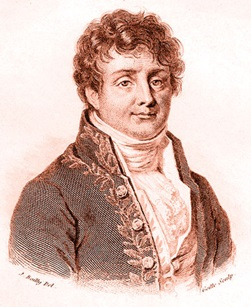
\includegraphics[scale=1]{fourier}
	\caption{Joseph Fourier.}
	\label{fig:fourier}
\end{figure}

\section{Bouwen aan begrip}

Fouriers interesse in algebra gaat u zeker terugzien, maar om daar te komen, is het belangrijk om een grondige intuïtie op te bouwen alvorens men de wiskundige berekeningen begrijpen kan. Laten we daarom bij het begin beginnen.

\subsection{Een punt}
De fouriertransformatie is het verhaal van een bewegende punt. Het beweegt in één dimensie. De horizontale dimensie. En het beweegt van links naar rechts en weer terug. De tijd dat het deeltje beweegt kan oneindig zijn, maar de functie die de positie van dit punt bepaalt, zorgt voor een slingerende beweging op de horizontale as van een assenstelsel. Dit is in feite de cosinusfunctie, die wel al eerder hebben gezien bij het uitleggen van de eenheidscirkel.
\begin{figure}[h]
	\centering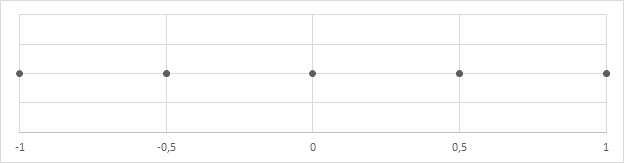
\includegraphics[scale=.8]{punt}
	\caption{Het punt op verschillende plaatsen.}
	\label{fig:punt}
\end{figure}

Zie in Fig. \ref{fig:punt} een paar posities van het punt dat beweegt volgens $\text{positie}=\cos{(\text{tijd})}$. De plaats van het punt op de horizontale as is dus de cosinus van het de tijd.

\subsection{Twee dimensies}
Maar dit ene punt was niet helemaal tevreden met het bestaan in maar één dimensie. Het wilde graag in meerdere dimensies bewegen. Maar wel in twee onafhankelijke. Nu komt er nog een extra functie bij die de plaats van het punt doet veranderen: $\text{verticale positie}=\sin{(\text{tijd})}$. Deze functie zorgt ook voor een slinger, maar dan op de verticale as.
\begin{figure}[h]
	\centering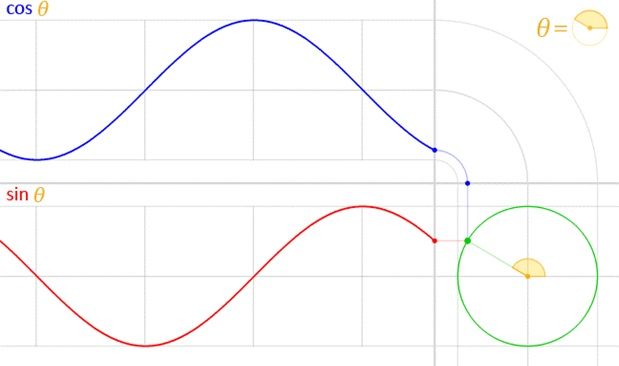
\includegraphics[scale=.8]{sincos}
	\caption{De sinus en cosinus vormen samen een cirkel.}
	\label{fig:sincos}
\end{figure}

Zo is het punt heen en weer, en op en neer t.o.v. de horizontale en verticale as aan het slingeren. Want de horizontale positie wordt bepaald door de cosinusfunctie en de verticale positie wordt bepaald door de cosinusfunctie. Dat is goed in de Fig. \ref{fig:sincos} te zien. Linksonder in het rood is de sinusfunctie afgebeeld en linksboven in het blauw de cosinusfunctie. Steeds bepalen ze samen een plaats waar de punt zich mag bevinden.

\subsection{Cirkelbeweging}
In feite kan op ieder moment in de tijd een punt beschreven worden m.b.v. de cosinus- en sinusfunctie samen. Wat men krijgt als alle punten aangegeven worden, is een cirkel. Er is dus sprake van een cirkelbeweging.

Nogmaals, de sinus en cosinus beschrijven respectievelijk de verticale en horizontale dimensies. Sinds wiskundigen dingen moeilijk willen maken, hebben ze speciale namen voor die dimensies. De horizontale dimensie noemen ze de reële as en de verticale dimensie noemen ze de imaginaire as. Gaat er nu een belletje rinkelen? Zo niet, kijk dan even naar Fig. \ref{fig:c-sincos} en vergelijk beide stelsels met elkaar.
\begin{figure}[h]
	\centering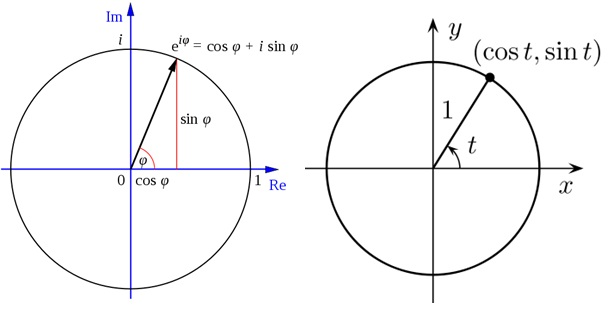
\includegraphics[scale=.8]{c-sincos}
	\caption{De eenheidscirkel naast de complexe eenheidscirkel.}
	\label{fig:c-sincos}
\end{figure}

\subsection{Rotatie}
Als we het over een punt hebben dat over een cirkel beweegt, dan is het ook belangrijk om wat te weten over de begrippen rotatie, tijd en snelheid. Roteren is zo simpel als ergens omheen draaien. Als men over de snelheid praat, dan praat men over de afstand dat iets aflegt in een bepaalde tijdsperiode. Je zou dus kunnen zeggen dat ons punt in één seconde de hele cirkel rond gaat.
\begin{displaymath}
	\text{snelheid}=\frac{\text{afstand}}{\text{tijd}},
\end{displaymath}
dus
\begin{displaymath}
	\text{snelheid}=\frac{2\pi r}{seconde}.
\end{displaymath}
Waarom de omtrek $2\pi r$ is, is eerder bewezen.

We hebben dus seconden in de noemer (de onderkant van de breuk) en omdat dat vaak gebeurt in de wis- en natuurkunde, hebben we daar een speciale naam voor bedacht. Die naam is hertz (Hz). Het is de eenheid van frequentie, of slingerende beweging.

Punten kunnen roteren met verschillende snelheden. Om dit een beetje intuïtief te maken is het goed om te kijken naar de analoge klok aan de muur. Het geeft de tijd aan met twee, maar soms drie wijzers: de uurwijzer, de minuutwijzer en de secondewijzer. Wat zichtbaar is, is dat alle wijzers met verschillende snelheden, frequenties, bewegen. Reken deze zelf eens uit aan de hand van onderstaande formules. Vul voor $r$ de afstand van het middelpunt tot de rand in.
\begin{displaymath}
	\text{frequentie uurwijzer}=\frac{2\pi r}{43200},\qquad \text{minuutwijzer}=\frac{2\pi r}{3600},\qquad \text{secondewijzer}=\frac{2\pi r}{60}.
\end{displaymath}

Wat meteen moet opvallen, is dat het aantal hertz van de uurwijzer kleiner is dan die van de minuutwijzer en de minuutwijzer heeft op zijn beurt weer een kleinere frequentie dan de secondewijzer.

Houd deze begrippen van punten over cirkels en klokwijzers vast. Die gaan we later nodig hebben.

\subsection{Data}
Laten we nu praten over data. Bekijk Fig. \ref{fig:data-1}. 
\begin{figure}[h]
	\centering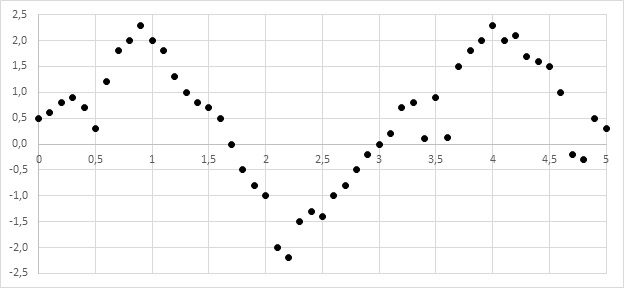
\includegraphics[scale=.8]{data-1}
	\caption{Een willekeurige dataset.}
	\label{fig:data-1}
\end{figure}

Deze data kan van alles zijn. De hartslag in een korte tijd, de waterspiegel in een jaar, de energie op de antenne van je telefoon in een seconde. Het kan alles zijn wat je meet op gefixeerde momenten in de tijd. Het wordt gemeten en daarna opgeslagen. Men heeft dan een mooie rij met metingen. De gemeten data is discreet. Dat wil zeggen dat variabelen los van elkaar zijn gemeten. Ze zijn dus ook nog eens gemeten op gefixeerde momenten.

\subsection{Frequentie}
Men heeft eigen metingen gedaan en weet daarom in wat voor tijdsinterval de metingen verricht zijn (jaren, maanden, dagen, uren, etc.). Dit tijdsinterval noemt men $T_s$ (spreek uit: "t's van s"). De letter $s$ staat hier voor seconden. We kunnen hier weer dat trucje met de snelheid, de frequentie, uitvoeren. De frequentie is
\begin{displaymath}
	\text{frequentie}=F_s=\frac{1}{T_s}.
\end{displaymath}
$F_s$ is dan de snelheid van de meting, of hoe vaak de meting per tijdseenheid uitgevoerd wordt.

\subsection{2D-projectie}
Dit is waar het interessant wordt. De data die we nu hebben, is in één dimensie. Dit is zo, want uit iedere meting komt een enkel punt. Als men data meet wilt men dit later analyseren. Dan wordt bijvoorbeeld gekeken naar het medium, de variantie, de distributie. Misschien maakt men er wel een histogram van om daar weer leuke dingen mee te doen. Of als er een afbeelding is om te analyseren, dan kan gekeken worden naar de groene, blauwe en rode 'kanalen'. Dit zijn allemaal manieren om naar de data te kijken en te bedenken of er een verband is dat bij de metingen hoort. Als men data heeft dat periodisch (herhalend) is, of men denkt dat het periodisch is, dan is kijken naar de frequentie een manier om de data te begrijpen. Men vraagt zich dan af wat de onderliggende periodische natuurlijkheid van de data is. Om daarachter te komen, moeten we eerst de eendimensionale data naar tweedimensionale data transformeren.

\begin{figure}[h]
	\centering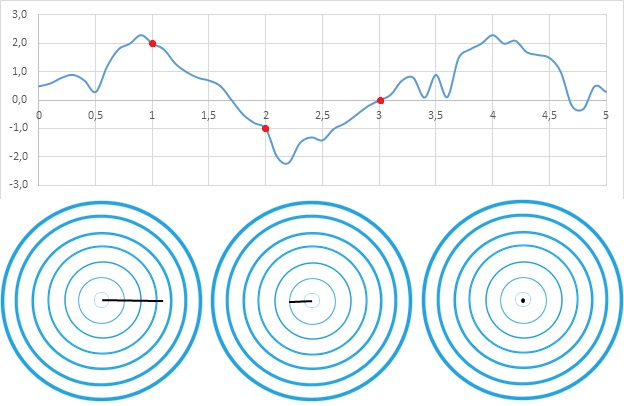
\includegraphics[scale=.8]{data-1-proj}
	\caption{De projectie van data op cirkels.}
	\label{fig:data-1-proj}
\end{figure}

We doen dit, door de data op cirkels te projecteren, zie Fig. \ref{fig:data-1-proj}. Met een beetje inbeeldingsvermogen lijken het net klokken. Deze klokken draaien in feite tegen de klok in met een zelfgekozen snelheid. Neem bij bovenstaande klokken maar aan dat $\text{frequentie}=1$. Dat betekend dat een punt in één seconde, een afstand van $2\pi$ aflegt (de omtrek is $2\pi$) . Wat te zien is in het diagram, is dezelfde data als die net besproken is. Dezelfde 'golf' van metingen. Er zijn een paar markeringen te zien. De rode stippen corresponderen van links naar rechts met de klokken. Ze indiceren een specifiek moment in de tijd. Op dat moment veranderen we de lengte van de klokwijzer, alsof het klokken waren. Zoals te zien is, is de wijzer lang als de meting hoog is. Als de meting nul is, dan heeft de wijzer ook geen lengte. En als de meting negatief is, dan draait de wijzer precies de andere kant op. De hoek die de wijzer maakt wordt bepaald door de frequentie. Men kan namelijk de frequentie van de klok zelf kiezen en dat geeft verschillen. Hierover later meer.

Wat belangrijk is om nu te zien, is dat dat ene punt nu niet alleen een punt is, maar een hele lijn is geworden. Het is zogezegd van eendimensionaal in tweedimensionaal veranderd. De meting was eendimensionaal als een punt op die golvende lijn en later tweedimensionaal op de klokken. Denk terug aan die cirkel met onafhankelijke verticale en horizontale dimensies.

De klokken met hun wijzers gaan nu alleen nog maar over specifieke momenten in de tijd, maar wat als we nu alle data op een enkele klok zouden projecteren. Omdat het vanaf hier moeilijker wordt om eigenhandig te illustreren, gebruik ik figuren die gemaakt zijn door William Cox \cite{cox}. Hij gebruikt ook andere data, dus die zal ik vanaf hier ook overnemen.

\begin{figure}[h]
	\centering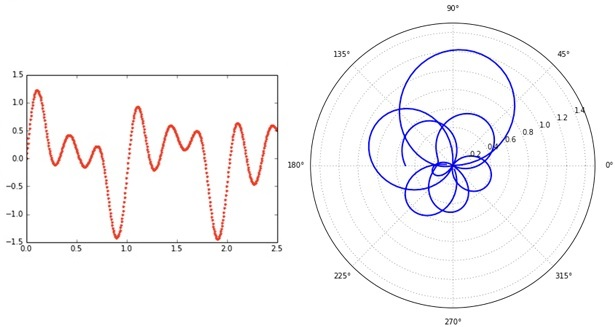
\includegraphics[scale=.8]{data-2-proj}
	\caption{Een andere willekeurige dataset dit geprojecteerd is op een 2D-vlak.}
	\label{fig:data-2-proj}
\end{figure}

Waar je naar kijkt in Fig. \ref{fig:data-2-proj}, is dezelfde soort grafiek als we al eerder gezien hebben. Deze is nu in het rood geschetst, maar nu zien we ook een diagram die ons minder bekend voorkomt. En toch lijkt het op iets wat we al eerder bekeken hebben. Het is een cirkel met daarin alle metingen. Eigenlijk is dit hetzelfde als we net zagen, die klokken met een enkele wijzer, maar nu staan alle gegevens erin als punten. Expres zijn de metingen nog niet als wijzers weergegeven, daar komen we zo op terug. Er is iets moois gebeurd. In plaats van dat er nu maar een enkele meting tweedimensionaal is geworden, hebben we nu alle data tweedimensionaal beschikbaar. Daar kunnen we leuke dingen mee doen.

Hierbij moet wel gezegd worden dat op de afbeelding, de frequentie vaststaat. Dat wil zeggen dat er één frequentie gekozen is om het diagram te plotten. Het is veel interessanter om te kijken naar wat er gebeurt als we de frequentie aanpassen. En wat blijkt, als de frequentie groter wordt, dan verspreid het signaal zich over de gehele cirkel. Dit is te zien in een latere figuur.

Maar wat is er nu met de tijd gebeurd? De tijd is veranderd in de positie van de wijzer rond de cirkel. De wijzer zal later in de tijd meer afstand afgelegd hebben dan wanneer hij net begonnen is. Eigenlijk is er vanaf nu dus geen sprake meer over tijd, maar over de positie van de wijzer.

\subsection{Vectoren}
Dus nu hebben we een hele hoop metingen in twee dimensies. Ieder punt leeft in twee dimensies en is dus een lijn. Zo'n lijn noemen we een vector. We kunnen vectoren bij elkaar optellen, zie Fig. \ref{fig:vec+}. Dat werkt als volgt. Men neme een vector $\vec{a}$ en een vector $\vec{b}$. Beide vectoren samen noemen we vector $\vec{c}$. Dus

\begin{displaymath}
	\vec{c}=\vec{a}+\vec{b}.
\end{displaymath}

\begin{figure}[h]
	\centering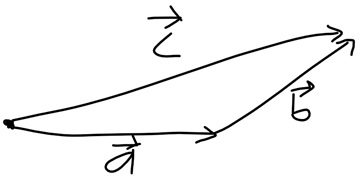
\includegraphics[scale=1]{vec+}
	\caption{Twee vectoren bij elkaar opgeteld.}
	\label{fig:vec+}
\end{figure}

Vectoren worden vaak weergegeven als $\begin{pmatrix}x \\ y\end{pmatrix}$ waarbij $x$ de verplaatsing in de x-richting is en y de verplaatsing in de y-richting. Dus in Fig. \ref{fig:vec+} zou het volgende van toepassing kunnen zijn.
\begin{displaymath}
	\vec{c}=\vec{a}+\vec{b}=\begin{pmatrix}3 \\ 0\end{pmatrix}+\begin{pmatrix}2 \\ 2\end{pmatrix}=\begin{pmatrix}5 \\ 2\end{pmatrix}
\end{displaymath}
Vector $\vec{c}$ heeft dan de verplaatsing $\begin{pmatrix}5 \\ 2\end{pmatrix}$.

Men kan een vector dus beschrijven als een verplaatsing in x- en y-richting, maar men kan een vector ook beschrijven als een lijn met een bepaalde lengte die een hoek maakt met de horizontale as, zoals in Fig. \ref{fig:vecal}. In de figuur zie je opnieuw de vector $\vec{c}$ die lengte $\sqrt{29}$ heeft en $\angle \alpha = 90^\circ$.

\begin{figure}[h]
	\centering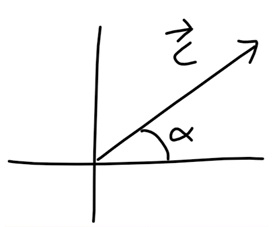
\includegraphics[scale=1]{vecal}
	\caption{Een vector gerepresenteerd bij lengte en hoek.}
	\label{fig:vecal}
\end{figure}

\subsection{Transformeren}
Terug naar de cirkel waar we al onze data op gezet hebben. Vanaf hier gaat het hard, dus wees gewaarschuwd. Gezegd was, dat de frequentie van de cirkel veranderd kon worden en dat daardoor verschillende figuren te zien zouden zijn. Dat beelden we in Fig. \ref{fig:data-2-proj-2} door de figuren te laten zien die horen bij een paar verschillende frequenties. Dit is te zien in de cirkels. De blauwe lijn bestaat uit al onze metingen die aan het begin van het onderzoek gemaakt zijn. Deze veranderd dus door het kiezen van andere frequenties. Steeds is rechtsboven de gemiddelde vector van alle vectoren te zien. Dit is als het ware alle vectoren bij elkaar opgeteld. Dus alle vectoren, punten die we tweedimensionaal gemaakt hebben door ze op een cirkel te projecteren, tellen we bij elkaar op zoals we dat eerder gedaan hebben. In plaats van twee vectoren, hebben we er nu vele malen meer, maar het principe werkt hetzelfde.

\begin{figure}[h]
	\centering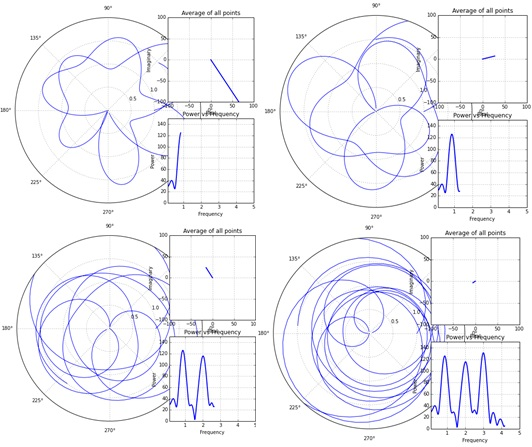
\includegraphics[scale=1]{data-2-proj-2}
	\caption{Projectie van de data met verschillende frequenties.}
	\label{fig:data-2-proj-2}
\end{figure}

Het vinden van zo’n gemiddelde vector is hetzelfde als het zwaartepunt van alle punten vinden en vervolgens een lijn vanaf het midden naar dat punt tekenen. Ligt het zwaartepunt ver van het midden af, dan is de lijn groot. Ligt 'ie richting het midden, dan zal de vector kleiner zijn. Doordat verschillende frequenties bekeken worden, zijn er ook verschillende gemiddelde vectoren. En zoals gezegd is deze gemiddelde vector uit te drukken in de hoek die het maakt en de lengte ervan. Met de lengte kunnen leuke dingen gedaan worden. Zo is het mogelijk om een nieuw diagram te maken die de kracht van een bepaalde frequentie kan aangeven. De kracht is afhankelijk van hoe lang de zwaartepuntvector is. Hoe langer de vector, hoe groter de kracht. De frequentie die bij de kracht hoort, die was vooraf al bepaald.

\subsection{Tijd- en frequentiedomein}
Het diagram dat ontstaat is steeds rechtsonder weergegeven. Er zijn drie duidelijke pieken te zien in de figuur. Dat zijn de frequenties die het meest aanwezig zijn in de data. Wat deze betekenen, daar komen we nog wel achter.

Zoals gezegd, is de horizontale as nu niet meer de tijd aan het aangeven, maar de frequentie. We zijn naar een ander domein gereisd door de fouriertransformatie. Namelijk van het tijd- naar het frequentiedomein \cite{fd}.

Simpel gezegd is het verschil tussen het tijd- en frequentiedomein dat een tijddomein-grafiek laat zien hoe een signaal veranderd in de tijd, terwijl een frequentiedomein-grafiek laat zien hoe veel van een signaal in een bepaald frequentiegebied ligt.

Dat laatste is in essentie wat de fouriertransformatie doet: een grafiek transformeren van het tijd- naar het frequentiedomein. Later zien we dat het ook andersom kan, dus van het frequentie- naar het tijddomein.

We hebben een stevig begrip gebouwd voor de fouriertransformatie. Dit is wat de fouriertransformatie doet, maar dan op een intuïtieve manier uitgelegd. Wat het nut is van de fouriertransformatie komen we later op. Eerst komt de achterliggende wiskunde aan bod.

\subsection{Harmonische frequenties}
We hebben gezien dat de getransformeerde de kracht van verschillende frequenties weergeeft. Maar wat stellen die frequenties ($\omega$) nou eigenlijk voor?

$\omega=0$ is het gemiddelde van alle frequenties. De fundamentele frequentie is de frequentie $\frac{2\pi}{NT} rad/sec$. Oftewel, de fundamentele frequentie is één rondje, gedeeld door het aantal metingen maal de tijd tussen metingen. Een harmonische is een veelvoud van deze fundamentele frequentie.

Ieder signaal dat periodisch is bestaat uit deze fundamentele en harmonische frequenties. De fundamentele frequentie wordt de eerste harmonische genoemd. Deze bepaalt het meest hoe het signaal eruitziet. De frequentie van de tweede harmonische is tweemaal de frequentie van de eerste harmonische. De derde drie keer zo groot als de eerste, etc.

\section{De passie van Fourier}
We weten nu goed wat er gebeurt als we de fouriertransformatie toepassen. Als je het op een signaal toepast, dan ga je van het tijd- naar het frequentiedomein. Andersom kan het ook, hadden we gezegd.

Neem nu Fig. \ref{fig:bas}. De eerste afbeelding toont het tijd-tegen-amplitudediagram van een basgitaar die een open snaar A-noot speelt (55 Hz). Daaronder is een andere afbeelding getoond die laat zien welke frequenties er aanwezig zijn in opname, in een frequentie-tegen-amplitudediagram. De verticale as van de onderste afbeelding is logaritmisch. Daaruit kun je opmaken dat de hogere frequenties sterk minder aanwezig zijn dan de lagere. Niet verrassend, want de 55 Hz toon die bespeeld werd, is laag.

\begin{figure}[h]
	\centering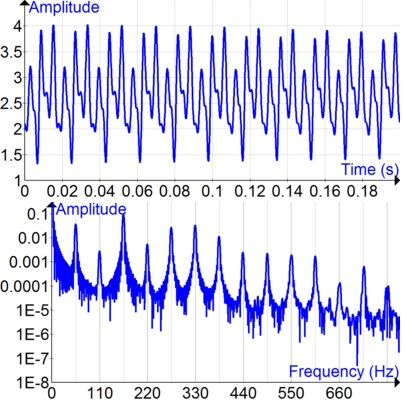
\includegraphics[scale=1]{bas}
	\caption{Open snaar A-noot van een basgitaar in respectievelijk het tijd- en frequentiedomein}
	\label{fig:bas}
\end{figure}

In deze sectie gaan we redelijk pittige wiskunde behandelen. Het is moeilijk om dit eenvoudig uit te leggen. Niet-wiskundig aangelegde mensen kunnen ervoor kiezen dit gedeelte over te slaan, hoewel dit wel een cruciaal deel is om de fouriertransformatie door en door te begrijpen.

\subsection{Fourierreeksen}
Stel je hebt een functie $f(x)$. Wat deze functie ook mag zijn, hoe raar ook, het is altijd mogelijk om hem te recreëren door sinussen en cosinussen herhaaldelijk aan elkaar te plakken \cite{fs}. Dit kan je oneindig doen zodat je een zo goed als perfecte benadering hebt van de oorspronkelijke functie. Wanneer je dit toepast, dan spreek je van een het maken van een fourierreeks.

Bekijk Fig. \ref{fig:fourierreeksen}. Hierin is een vierkante golf te zien. Deze wordt benaderd door een fourierreeks. Je ziet dat in het bovenste diagram eerst een grote globale rode lijn is getekend die al redelijk veel bepaald. Er zijn meerderen sinusoïden getekend. Steeds worden ze iets nauwkeuriger, maar opvallend is, is dat de bovenste wel heel duidelijk aangeeft waar de vierkante golf zich bevindt.

\begin{figure}[h]
	\centering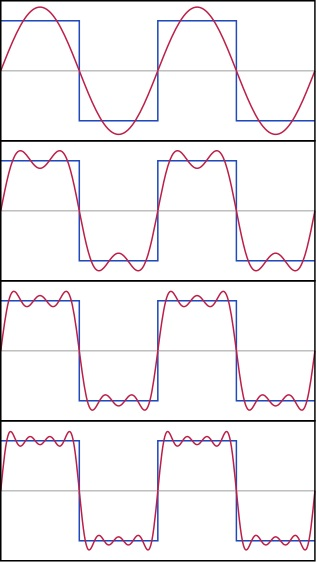
\includegraphics[scale=1]{fourierreeksen}
	\caption{Fourierreeksen.}
	\label{fig:fourierreeksen}
\end{figure}

Fourier kwam achter deze reeksen in zijn zoektocht naar het oplossen van de diffusievergelijking in een metalen plaat. Dit is een partiële differentievergelijking. Dat is een ander woord voor niet zo makkelijke wiskunde.

De fourierreeksen worden nu in zeer veel verschillende gebieden gebruikt. Hoewel het was bedacht om de diffusievergelijking op te lossing, werd de techniek toegepast op een breed scala aan andere wiskundige en natuurkundige problemen. Een paar van deze problemen zijn te vinden in studies als elektrotechniek, vibratieanalyse, akoestiek, optiek, signaalverwerking, digitale beeldbewerking, kwantummechanica, econometrie, etc. Het is eigenlijk te veel om op te noemen, maar het mag duidelijk zijn dat de heer Joseph Fourier een baanbrekende uitvinding heeft gedaan.

\subsection{Continue fouriertransformatie}
Een fourierreeks is dus een stapel sinusoïden die samen een functie bijna exact benaderen. Ook weten we inmiddels dat we kunnen veranderen tussen tijd- en frequentiedomein. Hoe dat laatste moet, daar gaan we het nu over hebben.

De vergelijkingen die zo te zien zijn, zijn continue fouriertransformaties. Dit zijn de echte, of basis. Continu wil zeggen dat we rekenen met functies of ononderbroken lijnen zoals in Fig. \ref{fig:fx}.

\begin{figure}
\centering
\definecolor{cqcqcq}{rgb}{0.7529411764705882,0.7529411764705882,0.7529411764705882}
\begin{tikzpicture}[line cap=round,line join=round,>=triangle 45,x=1.0cm,y=1.0cm]
\draw [color=cqcqcq,, xstep=1.0cm,ystep=1.0cm] (-2.,-2.) grid (2.,2.);
\draw[->,color=black] (-2.,0.) -- (2.,0.);
\foreach \x in {-2.,-1.,1.}
\draw[shift={(\x,0)},color=black] (0pt,2pt) -- (0pt,-2pt) node[below] {\footnotesize $\x$};
\draw[->,color=black] (0.,-2.) -- (0.,2.);
\foreach \y in {-2.,-1.,1.}
\draw[shift={(0,\y)},color=black] (2pt,0pt) -- (-2pt,0pt) node[left] {\footnotesize $\y$};
\draw[color=black] (0pt,-10pt) node[right] {\footnotesize $0$};
\clip(-2.,-2.) rectangle (2.,2.);
\draw[line width=2.pt,smooth,samples=100,domain=-2.0:2.0] plot(\x,{(\x)^(3.0)+(\x)});
\begin{scriptsize}
\draw[color=black] (-1.34,-5.37) node {$f$};
\end{scriptsize}
\end{tikzpicture}
\caption{Een continue functie.}
\label{fig:fx}
\end{figure}

Naar de rekentafel. Laat $f(x)$ een functie zijn van een reële variabele $x$. De continue fouriertransformatie van $f(x)$ is dan Vgl. \ref{eq:cf}.
\begin{definition}[Continue fouriertransformatie]\label{eq:cf}
De continue fouriertransformatie wordt gegeven door
\begin{align}
\hat{f}(\xi)=\int_{-\infty}^\infty f(x)e^{i2\pi \xi x} \, dx
\end{align}
\end{definition}

waar $i = \sqrt{-1}$ \cite{yy}. De getransformeerde wordt vaak aangeduid met een dakje op de functienaam. De Griekse letter xi ($\xi$) representeert frequentie. Als $x$ in seconden is, dan is $\xi$ in hertz. Er is sprake van een integraalrekening\footnote{Lees meer over integraalrekeningen in \cite{int}}. Men ziet graag een min in de exponent. Dit houdt in dat we met de klok mee om de projectiecirkel (denk even terug) draaien. u wordt vaak de frequentievariabele genoemd. Bij het kijken naar deze vergelijking is niet meteen duidelijk dat het om optellen van sinussen en cosinussen gaat. Dat wordt wel anders als we Eulers vergelijking in de strijd gooien. Dit geeft
\begin{equation*}
\hat{f}(\xi)=\int_{-\infty}^\infty f(\cos{(2\pi \xi x)}-i\sin{(2\pi \xi x)})\, dx.
\end{equation*}
Met $\hat{f}(\xi)$ gegeven, kunnen we achteruit en de $f(x)$ krijgen door de inverse continue fouriertransformatie.
\begin{definition}[Inverse continue fouriertransformatie] \label{eq:icf}
De inverse continue fouriertransformatie wordt gegeven door
\begin{align}
f(x)=\int_{-\infty}^\infty \hat{f}(\xi)e^{i2\pi \xi x} \, dx.
\end{align}
\end{definition}

$f(\xi)$ en $f(x)$ heten samen het fouriertransformatiepaar en ze bestaan als $f(x)$ continu (zonder stop) en te integreren is (als er een oppervlakte onder de grafiek is), en $f(\xi)$ te integreren is. Als je voor $f(\xi)$ een min in de exponent kiest, dan moet je bij $f(x)$ een plus in de exponent kiezen.
$f(\xi)$'s zijn de data in het frequentiedomein. Stel je hebt een reële functie $f(x)$ in het tijddomein, dan komt je op complexe waarden van $f(\xi)$ uit. Dit omdat een reëel getal maal een complex getal een complex getal is. Nu we hebben vastgesteld dat $f(\xi)$ complex is kunnen we stellen dat
\begin{equation*}
\hat{f}(\xi)=\Re + i\Im
\end{equation*}
Deze vergelijking hebben we eerder gezien. $\Re$ is het reële deel en $\Im$ het imaginaire.

\subsection{Discrete fouriertransformatie}
Nu we iets weten over de echte wiskundigheid achter de fouriertransformatie, moeten we een manier vinden om het toe te passen. Denk terug aan toen we een signaal gingen transformeren in de vorige sectie. We hebben zojuist gelezen dat een signaal continu moet zijn om het te kunnen transformeren. Helaas. Wees niet getreurd, want wiskundigen hebben hier een oplossing voor bedacht: de discrete fouriertransformatie (DFT).

De DFT is equivalent aan de continue FT. Het verschil is dat de DFT alleen bedoeld is voor gesamplede (bemonsterde) signalen. Integendeel tot de continue behandeld de DFT-data alsof het periodisch is en is dus geschikt voor een eindig aantal samples.

Gegeven zijn $N$ (een geheel aantal) metingen van $f(x)$. De metingen zijn verricht in gefixeerde intervallen. Er zijn dan vergelijkingen die Vgl. \ref{eq:cf} en \ref{eq:icf}.
\begin{definition}[Discrete fouriertransformatie] \label{eq:dft}
De discrete fouriertransformatie wordt gegeven door
\begin{align}
\hat{f}(\xi)=\sum_{x=0}^{N-1} f(x)e^{\frac{-i2\pi \xi x}{N}}
\end{align}
voor $\xi=\{0, 1, 2, \ldots, N-1\}$.
\end{definition}
\begin{definition}[Inverse discrete fouriertransformatie] \label{eq:idft}
De inverse discrete fouriertransformatie wordt gegeven door
\begin{align}
f(x)=\sum_{x=0}^{N-1} \hat{f}(\xi)e^{\frac{i2\pi \xi x}{N}}
\end{align}
voor $x=\{0, 1, 2, \ldots, N-1\}$.
\end{definition}


Vgl. \ref{eq:dft} en \ref{eq:idft} heten respectievelijk de DFT en de IDFT. Omdat de operatie data behandeld alsof het periodisch is, gebruiken we de fundamentele frequentie en zijn harmonische frequenties. Het gemiddelde van alle frequenties ligt op $\xi=0$. Merk op dat de integraal is vervangen voor het sommatieteken\footnote{Lees meer over dit teken in \cite{som}}.

De berekening in $\Sigma$ is
\begin{displaymath}
\begin{aligned}
f\cdot e^{\frac{i2\pi \xi x}{N}}&=(R+iI)\cdot(\cos{(p)}-\sin{(p)})\\
& = R\cos{(p)}-iR\sin{(p)}+iI\cos{(p)}-i^2I\sin{(p)}\\
& =R\cos{(p)}-iR\sin{(p)}+iI\cos{(p)}-I\sin{(p)}\\
& =(R\cos{(p)}+I\sin{(p)})+i(I\cos{(p)}-R\sin{(p)}),
\end{aligned}
\end{displaymath}
waar $R$ en $I$ reële getallen zijn, $I=0$ als $f$ een reëel getal is. $p=2\pi\xi x$.

\subsection{Een rekenvoorbeeld}
Bekijk het volgende signaal.
\begin{equation*}
f(x)=6+4\cos{\left(\pi t - \frac{1}{2}\pi\right)}+3\cos{\left(3\pi t\right)}
\end{equation*}

In Fig. \ref{fig:fx2} staat de grafiek samen met zijn onderdelen geplot.

\begin{figure}
\centering
\scalebox{0.6}{
\definecolor{ffdxqq}{rgb}{1.,0.8431372549019608,0.}
\definecolor{qqffqq}{rgb}{0.,1.,0.}
\definecolor{ffqqqq}{rgb}{1.,0.,0.}
\definecolor{cqcqcq}{rgb}{0.7529411764705882,0.7529411764705882,0.7529411764705882}
\begin{tikzpicture}[line cap=round,line join=round,>=triangle 45,x=2.5cm,y=0.5555555555555556cm]
\draw [color=cqcqcq,, xstep=12.5cm,ystep=2.7777777777777777cm] (-1.,-5.) grid (7.,13.);
\draw[->,color=black] (-1.,0.) -- (7.,0.);
\foreach \x in {,5.}
\draw[shift={(\x,0)},color=black] (0pt,2pt) -- (0pt,-2pt) node[below] {\footnotesize $\x$};
\draw[->,color=black] (0.,-5.) -- (0.,13.);
\foreach \y in {-5.,5.,10.}
\draw[shift={(0,\y)},color=black] (2pt,0pt) -- (-2pt,0pt) node[left] {\footnotesize $\y$};
\draw[color=black] (0pt,-10pt) node[right] {\footnotesize $0$};
\clip(-1.,-5.) rectangle (7.,13.);
\draw[line width=2.pt,smooth,samples=100,domain=-1.0:7.0] plot(\x,{3*cos((3*3.1415926535*(\x))*180/pi)+4*cos((3.1415926535*(\x)-1/2*3.1415926535)*180/pi)+6});
\draw [line width=2.pt,dotted,color=ffqqqq,domain=-1.:7.] plot(\x,{(--6.-0.*\x)/1.});
\draw[line width=2.pt,dotted,color=qqffqq,smooth,samples=100,domain=-1.0:7.0] plot(\x,{4*cos((3.1415926535*(\x)-1/2*3.1415926535)*180/pi)});
\draw[line width=2.pt,dotted,color=ffdxqq,smooth,samples=100,domain=-1.0:7.0] plot(\x,{3*cos((3*3.1415926535*(\x))*180/pi)});
\begin{scriptsize}
\draw[color=black] (-10.658136879300798,8.606271382829053) node {$f$};
\draw[color=ffqqqq] (-10.658136879300798,5.5342388190584435) node {$h$};
\draw[color=qqffqq] (-10.658136879300798,1.5064627910036414) node {$p$};
\draw[color=ffdxqq] (-10.658136879300798,0.004580204271342536) node {$q$};
\end{scriptsize}
\end{tikzpicture}}
\caption{Functie $f(x)$, geplot.}
\label{fig:fx2}
\end{figure}

Laten we $f(x)$ vier maal per seconde samplen ($f_s=4$) van $t=0$ tot $t=3/4$. De waarden van de discrete samples zijn gegeven door
\begin{displaymath}
f(k)=6+4\cos{\left(\frac{1}{4}\pi k -\frac{1}{2}\pi\right)}+3\cos{\left(\frac{3}{4}\pi k\right)}\qquad\text{met}\qquad t=kT_s=\frac{k}{4}.
\end{displaymath}
Invullen van de vier samples geeft dan
\begin{displaymath}
f(k)=\begin{pmatrix}f(0)\\f(1)\\f(2)\\f(3)\end{pmatrix}\approx \begin{pmatrix}9\\6,7\\10\\10,9\end{pmatrix}.
\end{displaymath}

Hier demonstreren we hoe we de DFT van $f(x)$ berekenen \cite{sr}. Daarbij gebruiken we matrixen\footnote{Lees meer over matrixen in \cite{mat}} en rekenen we met de waarden van $f(k)$ alsof ze niet afgerond zijn.
\begin{displaymath}
\begin{aligned}
\hat{f}(0)&=e^{-i2\pi 0\cdot\frac{0}{4}}\cdot 9+e^{-i2\pi 0\cdot\frac{1}{4}}\cdot 6,7+e^{-i2\pi 0\cdot\frac{2}{4}}\cdot 10+e^{-i2\pi 0\cdot\frac{3}{4}}\cdot 10,9=36,7\\
\hat{f}(0)& =e^{-i2\pi 1\cdot\frac{0}{4}}\cdot 9+e^{-i2\pi 1\cdot\frac{1}{4}}\cdot 6,7+e^{-i2\pi 1\cdot\frac{2}{4}}\cdot 10+e^{-i2\pi 1\cdot\frac{3}{4}}\cdot 10,9=-1+4,2i\\
\hat{f}(0)& =e^{-i2\pi 2\cdot\frac{0}{4}}\cdot 9+e^{-i2\pi 2\cdot\frac{1}{4}}\cdot 6,7+e^{-i2\pi 2\cdot\frac{2}{4}}\cdot 10+e^{-i2\pi 2\cdot\frac{3}{4}}\cdot 10,9=1,3\\
\hat{f}(0)& =e^{-i2\pi 3\cdot\frac{0}{4}}\cdot 9+e^{-i2\pi 3\cdot\frac{1}{4}}\cdot 6,7+e^{-i2\pi 3\cdot\frac{2}{4}}\cdot 10+e^{-i2\pi 3\cdot\frac{3}{4}}\cdot 10,9=-1-4,2i
\end{aligned}
\end{displaymath}
Dit geeft ons de matrix
\begin{displaymath}
\hat{f}(\xi)=\begin{pmatrix}\hat{f}(0)\\\hat{f}(1)\\\hat{f}(2)\\\hat{f}(3)\end{pmatrix}=\begin{pmatrix}36,7\\-1+4,2i\\1,3-1-4,2i\end{pmatrix}.
\end{displaymath}

Deze matrix is mooi, want nu kunnen we een diagram maken (Fig. \ref{fig:trans}) die ons vorige diagram (Fig. \ref{fig:fx2}) omzet naar het frequentiedomein. De sterkte van de verschillende frequenties is daarin goed te zien.

\begin{figure}[h]
	\centering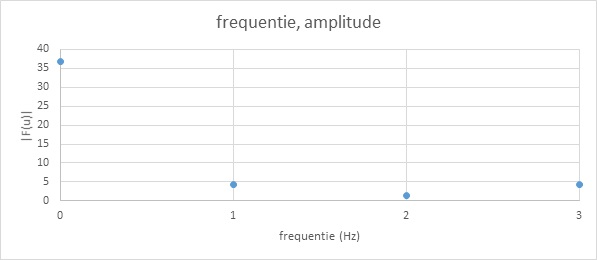
\includegraphics[scale=.8]{trans}
	\caption{Het frequentiespectrum.}
	\label{fig:trans}
\end{figure}

De sterkte van de frequenties is bepaald door de absolute waarde van de $f(\xi)$'s te nemen. Dat kan met modulusstrepen. De absolute waarde van $f(\xi)$ in de grafiek is $\left|F(u)\right|$. Zie Vgl. \ref{eq:abs} op pagina \pageref{eq:abs}.

Ziezo, daar heb je het. We hebben nu de functie $f(x)$ met het tijddomein veranderd in een matrix van $f(\xi)$-waarden. We zien nu de natuurlijke periodiek achter ons signaal. We kunnen nu zeggen dat sinusoïden met frequenties van 1 en 3 Hz meer aanwezig zijn dan met 2 Hz. Oftewel, de fundamentele frequentie is 1 Hz.

Natuurlijk had het veel nauwkeuriger gekund. Als we naar het signaal $f(x)$ kijken, zien we dat het een periode heeft van 2. Ook zien we verschillende pieken op verschillende momenten binnen zo’n periode. Je zou dus zeggen dat vier monsters nemen van $t=0$ tot $t=3/4$ minder nauwkeurig is dan op iedere kwart van $t$. In dit geval hadden we veel meer data gehad en meer pieken kunnen zien in het frequentiedomein. Zo had de analyse van dit signaal nog preciezer gegaan kunnen zijn.

We weten nu niet alleen wat er gebeurt als we een FT zien, we kunnen hem nu ook berekenen d.m.v. de DFT. Natuurlijk kan je m.b.v. de IDFT weer terug naar het tijddomein. Omdat deze berekening zo goed als op dezelfde wijze gaat, laten we deze hier niet zien. Als men deze IDFT toepast dan krijgt men niet exact hetzelfde signaal als die we eerst hadden, maar een fourierreeks daarvan. Zoals eerder gezegd  betekend dat, dat het signaal wordt benaderd door een stapel cosinussen en sinussen. Oftewel: de IDFT van $f(\xi)$ geeft een fourierreeks voor $f(x)$.

\section{Praktische toepassingen}
Allemaal leuk en aardig, zo’n fouriertransformatie, maar uiteindelijk moet men er toch iets mee kunnen. Voor de mensen die de wiskunde alleen maar saai, moeilijk of vervelend vinden, is er ook hoop. De FT is er niet voor niets en daarom bespreken we ook nog de toepassingen van de fouriertransformatie. Om tot die toepassingen te komen, moeten we het ook heel even over de Fast Fourier Transform hebben.

\subsection{Vliegensvlugge Fourier}
Vroeger, toen wiskunde in het bedrijfsleven nog veel met de hand gedaan werd, was het heel normaal om gegevens van het tijd- naar het frequentiedomein te veranderen m.b.v. de hand. "Nu we in een tijd leven waarin we beschikking hebben tot computers, moet het toch anders kunnen", dachten Cooley en Tukey, twee informatici, in 1965. Dit werd waarheid, want even later publiceerden zij samen de Fast Fourier Transform (FFT) evenals de inverse hiervan (IFFT) \cite{fft}. Dit zijn algoritmen die de transformaties zeer snel kunnen uitvoeren. Algoritmen zijn stukjes computercode die een computer uitvoert om een bepaalde handeling uit te voeren. We gaan het niet hebben over hoe de FFT werkt. Als hier interesse in is, bekijk dan zeker de Wikipediapagina 'Cooley-Tukey FFT Algorithm'.

\begin{figure}[h]
	\centering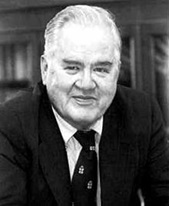
\includegraphics[scale=1]{tukey}
	\caption{John Tukey.}
	\label{fig:tukey}
\end{figure}

Tukey kwam op het idee toen hij een meeting had van president Kennedy’s Science Advisory Committee waar een discussie gaande was over het detecteren van nucleaire tests van de Sovjet-Unie. Slimmerds hadden bedacht dat dit wel met sensoren kon. Ze zaten niet fout, want Tukey kwam al snel met een het computeralgoritme om het uitgaande signaal om te zetten naar een analyseerbaar signaal. Mooi!

Richard Garwin was wel geïnteresseerd in Tukey’s trucje en vroeg naar details. Hij heeft het algoritme gebruikt voor van alles wat hem interesseerde. O.a. de periodiciteit van de spinoriëntaties in een 3D kristal van Helium-3. Garwin gaf Tukey’s ideeën aan Cooley die samen met Garwin bij IBM (een groot computerbedrijf) werkten. Cooley implementeerde het in nog een aantal andere dingen. Cooley en Tukey publiceerden zes maanden na de uitvinding een paper en omdat Tukey niet voor IBM werkte was het niet eerlijk om het patent aan IBM te geven. Daarom ging het algoritme in het publieke domein. Dat wil zeggen dat iedereen op de wereld het algoritme mag gebruiken zoals gewenst. Dit was bijzonder mooi voor de computerrevolutie. De FFT was voornamelijk het belangrijkste algoritme in de signaalanalyse.

In 2012 is een nieuwe grote verbetering op de FFT bedacht. Een stelletje MIT-onderzoekers hebben de Sparse Fourier Transform (SFT) uitgevonden. Met de SFT kan data tien tot honderd keer sneller data worden verwerkt.

Nu we wat over deze geschiedenis weten, laten we naar verschillende gebruiken hiervan kijken.

\subsection{Audio}
Audio is te vinden in verschillende vormen en maten. Zo zijn er bijvoorbeeld FLAC-, WAV- en mp3-bestanden. WAV-bestanden zijn vrij groot. Dit komt doordat zij ook informatie bevatten over noten/tonen die een mens niet of nauwelijks kan horen, omdat ze zo laag of hoog zijn. Dit kost ruimte bij het opslaan van een liedje. Daarom dacht iemand: "Laten we het bestand verkleinen door de hoge en lage tonen weg te filteren".

Neem een WAV-bestand waarin uw favoriete muziek klinkt. Verdeel het in kleine brokjes muziek, segmenten. Pas nu een vorm van de fouriertransformatie toe op ieder segment. Dit zorgt ervoor dat van ieder segment de geluidsgolven worden omgezet naar de noten die er gespeeld worden. Het leuke is dat men nu kan kijken naar hoeveel iedere noot meedoet in de muziek. Sommige zijn, zoals gezegd, niet essentieel, aangezien ze meestal niet hoorbaar zijn voor de mens. Dump deze noten. Wat men overhoudt is een spectrum in het frequentiedomein met noten die hoorbaar zijn en essentieel voor de muziek. Transformeer deze weer terug naar het tijddomein en je hebt een kleiner bestandsformaat.

Geluid in brokjes verdelen is een principe dat Shazam ook gebruikt. Shazam is een app op de smartphone die muziek in de omgeving zeer snel herkent. Als je de app opent en op ‘luisteren’ drukt, dan begint het proces. De applicatie neemt geluid uit de omgeving op met een microfoon. Wat men krijgt is een geluidsgolf. Zoals we weten, kan deze golflengte getransformeerd worden met de FFT. Wat men krijgt is een golf die we nu een 'fingerprint' noemen. Vervolgens scant Shazam zijn database, op zoek naar een getransformeerde die zo goed als hetzelfde is \cite{shazam}. Heeft de app deze gevonden, dan weet je welke muziek er op dat moment klinkt. 

Filtering is ook een belangrijke toepassing. Het lijkt op het comprimeren, maar is werkt net iets anders. I.p.v. noten wegfilteren die niet hoorbaar zijn, kan je ook tonen wegfilteren die zeer vervelend zijn. Stel een filmmaker voor die voornamelijk in de buitenlucht opneemt. Buiten zijn veel geluiden. Sommige zullen de filmervaring belemmeren. Denk bijvoorbeeld aan een hoge piep of een ruis. Door te kijken naar de fouriertransformatie kan men zien welke pieken er in het geluid zijn. Vervolgens kan men pieken wegfilteren zodat ze achteraf niet meer hoorbaar zijn \ref{fig:filter}. Dit principe kan ook worden gebruikt bij afbeeldingen \cite{fc}.

\begin{figure}[h]
	\centering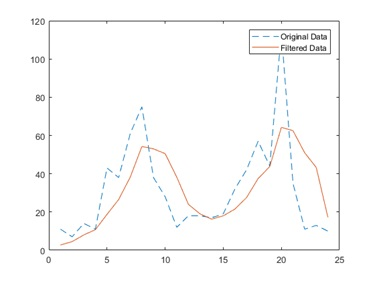
\includegraphics[scale=1]{filter}
	\caption{Filtering.}
	\label{fig:filter}
\end{figure}

\subsection{Astronomie}
Soms stuit men op een probleem. Problemen zijn er om opgelost te worden. Zo wilde NASA, een ruimtevaartorganisatie, de planeet Venus bekijken \cite{jg}. Venus staat relatief dichtbij aarde en zou daarom makkelijk met de telescoop te zien zijn. Helaas bleek dit niet zo te zijn, omdat het oppervlak zo goed als volledig bedekt is met wolken. Een telescoop kan niet door wolken heen prikken, dus moest er een andere manier verzonnen worden om Venus te kunnen bekijken.

NASA lanceert een satelliet, genaamd Magellan. Het is uitgerust met een radar en geavanceerde digitale signaalverwerkingssoftware. De satelliet is erop gemaakt om door wolken heen te kunnen 'kijken'. De missie van Magellan was om Venus op de kaart te zetten. De plaatjes die Magellan terugstuurde naar de aarde waren plaatjes als Fig. \ref{fig:venus}.

\begin{figure}[h]
	\centering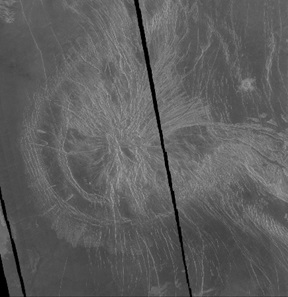
\includegraphics[scale=.6]{venus}
	\caption{Een oude afbeelding van Venus.}
	\label{fig:venus}
\end{figure}

Dit is een gedeelte van Venus. 20km breed. De zwarte strepen zijn enkel foutjes bij het maken van de afbeelding. De satelliet heeft veel meer kunnen doen dan verwacht. Het heeft 99\% van de totale oppervlakte van Venus in kaart gebracht. Van deze kaart en informatie van nog andere satellieten en ruimtevaartuigen, kon Fig. \ref{fig:venus2} worden gemaakt.

\begin{figure}[h]
	\centering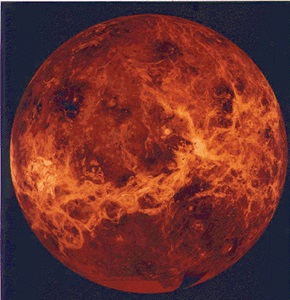
\includegraphics[scale=.6]{venus2}
	\caption{Constructieafbeelding van Venus.}
	\label{fig:venus2}
\end{figure}

Magellan had ook een kleine antenne die recht naar de oppervlakte wees. Deze mat de exacte tijd van hoelang het signaal erover deed om terug te komen bij de satelliet. Deze data en de eerdere kaarten hebben voor een spetterende animatie gezorgd die te downloaden is via \cite{jg}. Deze hele missie was zonder Fourier waarschijnlijk nooit zo succesvol geweest.

\subsection{Er is nog veel meer...}
Het blijft niet alleen bij geluid, afbeeldingen en astronomie. Er zijn veel meer toepassingen te bedenken voor deze transformatie. Hier volgt een opsomming van verschillende toepassingen en toepassingsgebieden. Klinkt iets interessant? Zoek het dan op!
De fouriertransformatie wordt ook toegepast op, maar is niet gelimiteerd aan: ontwerp en gebruik van antennes; transformatie, representatie en versleuteling; glad en scherp maken; restauratie, blur-verwijdering en Wiener filter; dataverwerking en analyse; seismologie; interferometers (VLBI of GPS); Synthetic Aperture Radar (SAR) en Interferometric SAR (InSAR); automotive; telecommunicatie; vibratie; optische natuurkunde; geologie; leger; astronomie \cite{in}\cite{gp}.

%----------------------------------------------------------------------------------------
%	CHAPTER 5
%----------------------------------------------------------------------------------------

\chapter{Kwantum superpositie van elementaire deeltjes}
In dit hoofdstuk gaan we kijken naar de toepassing van het complex getal in de vergelijking van Schrödinger. Maar voor we de vergelijking zelf gaan bekijken gaan we eerst naar het idee van de vergelijking kijken om zo hopelijk met een beter begrip naar de vergelijking te kijken. Of dit gaat lukken is de vraag want de vergelijking van Schrödinger is een complex stukje wiskunde wat in het middelpunt staat van een zeer complexe tak van de natuurkunde, namelijk de kwantummechanica. Kwantummechanica is een nog jong en snelgroeiend onderdeel van de natuurkunde, waar natuurkundigen als Einstein en Schrödinger een grote bijdrage aan hebben geleverd. Desondanks zijn we nog ver weg van een goed begrip van kwantummechanica, omdat het vaak niet te beschrijven is in termen die we herkennen uit de klassieke natuurkunde of ons dagelijks leven. Maar voor we hieraan beginnen gaan we eerst wat achtergrond schetsen van de situatie.

\section{Wie was Erwin Schrödinger?}
Erwin Rudolf Josef Alexander Schrödinger was geboren op 12 augustus 1887 in Wenen in het toenmalige Oostenrijk-Hongarije (tegenwoordig Oostenrijk). Zijn ouders waren Rudolf Schrödinger, een botanist, en Georgine Emilia Brenda Schrödinger, een scheikundeprofessor bij Technische Hochschule Vienna. Schrödinger was enig kind. Ondanks te zijn opgegroeid in een religieus gezin was Schrödinger zelf een atheïst, al had hij wel interesse voor oosterse religies.
\begin{figure}[h]
	\centering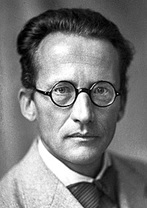
\includegraphics[scale=1]{erwin}
	\caption{Erwin Schrödinger}
	\label{fig:erwin}
\end{figure}
Schrödinger studeerde van 1906 tot 1910 onder Frans S. Exner en Friedrich Hasenöhrl en is in 1911 een assistent van Exner geworden. In 1914 begon Schrödinger het proces om zelf professor te worden, wat hij in 1921 afrondde. Op 6 april 1920 trouwde Erwin Schrödinger met de 23-jarige Annemarie Bertel. In 1921 is hij verhuisd naar Zürich waar hij ging werken bij de Universiteit van Zürich. 
Schrödinger publiceerde in januari 1926 het artikel "Quantisierung als Eigenwertproblem" in het wetenschappelijke blad "Annalen de Physik". Hierin maakte hij de golffunctie, die nu bekend staat als de Schrödingervergelijking, bekend. In de hierop volgende maanden publiceerde hij nog enkele artikelen die verschillende problemen en toevoegingen voor de golffunctie gaven. Deze artikelen waren revolutionair voor de kwantummechanica en zijn vierde artikel was waarschijnlijk de reden dat de kwantummechanica complexe getallen ging gebruiken in plaats van reële getallen.
In 1927 volgde hij Max Planck op bij de Universiteit van Berlijn. Hier werkt hij tot 1934, toen verliet hij Duitsland vanwege het opkomende antisemitisme van de Nazi's. Schrödinger is toen aan het werk gegaan bij de Universiteit van Oxford. Niet lang nadat hij was gaan werken in Oxford ontving hij een Nobelprijs samen met Paul Dirac voor zijn werk over de atoomtheorie: het idee dat materie bestaat uit een vast te stellen aantal atomen. Vanwege Schrödingers ongewone thuissituatie, hij woonde samen met zijn vrouw en zijn minnares, had hij problemen met verdere carrière maken in het Verenigd Koninkrijk. Uiteindelijk is hij in 1936 bij de Universiteit van Graz in Oostenrijk aan de slag gegaan. Gedurende deze periode had Schrödinger ook een brievenwisseling met Albert Einstein, waarin hij zijn bekende denkexperiment "Schrödingers kat" beschreef, waarmee hij de Kopenhagen-interpretatie van de kwantummechanica (dit wordt later verder besproken) in twijfel trok.
Toen in 1938 Oostenrijk werd opgenomen in Nazi-Duistland kwam Schrödinger in de problemen. Hij was Duitsland ontvlucht in 1933 en was een bekend tegenstander van het Nazisme. Hij probeerde zijn eerdere uitingen tegen de Nazi’s nog terug te nemen, waar hij later spijt van had, om zijn positie bij de Universiteit van Graz te behouden, maar dit was niet genoeg. Schrödinger werd ontslagen en vluchtte uiteindelijk naar Italië. Datzelfde jaar werd hij door de premier van Ierland gevraagd om te helpen met het opzetten van het Instituut voor Geavanceerde Wetenschappen in Dublin. Schrödinger verhuisde dus naar Dublin en werd in 1940 directeur van de School voor Theoretische Fysica. Gedurende zijn tijd in Dublin schreef Schrödinger zo’n 50 wetenschappelijke artikelen die verschillende wetenschappers inspireerden tot grootste ontdekkingen. Zo inspireerde Schrödingers artikel "What is Life?" James D. Watson en Francis Crick tot het onderzoeken van de functie en bouw van het DNA, wat leidde tot belangrijke doorbraken in de biologie.
In 1956 is Schrödinger teruggegaan naar Wenen. Hier leefde hij tot zijn overlijden op 4 januari in 1961. Erwin Rudolf Josef Alexander Schrödinger, de vader van de kwantummechanica, is 73 jaar oud geworden.

\section{De interpretatie van de kwantummechanica}
De reden dat Erwin Schrödinger met zijn vergelijking kwam, was om een wiskundige interpretatie te geven voor de verschijnselen die werden waargenomen in de kwantummechanica. Maar er waren natuurlijk ook theoretische verklaringen gegeven die probeerden te omschrijven wat er nou precies gebeurt. En voordat we met de Schrödingervergelijking gaan worstelen gaan we eerst kijken wat we nou proberen te berekenen.
Het probleem bij de kwantummechanica is dat deeltjes op een minuscuul niveau zich bij de ene meting als deeltjes lijken te gedragen en zich bij de andere meting als golven lijken te gedragen. Dit werd het duidelijkst bij het foto-elektrisch effect en bij het dubbele spleet experiment.

\subsection{Foto elektrisch effect}
Toen wetenschappers licht op een stukje metaal lieten schijnen merkten ze iets opvallends. Bij bepaalde lichtfrequenties (licht met een bepaalde golflente) werden er elektronen uit het metaal gekaatst. Dit was raar omdat men voorheen dacht dat licht als golf geen massa had en dus niet tegen de elektronen kon aanbotsen om ze weg te schieten. Eerst dachten ze dat het licht de elektronen opwarmde totdat die dan uiteindelijk wegschoten, maar dan zouden de elektronen sneller moeten wegschieten bij een hoge amplitude van de lichtgolven en zouden er meer moeten weg  schieten bij een hogere frequentie. Dit gebeurde echter niet per se. 
\begin{figure}[h]
	\centering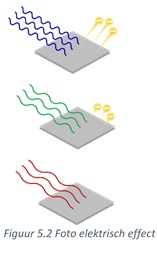
\includegraphics[scale=1]{fee}
	\caption{Foto elektrisch effect.}
	\label{fig:fee}
\end{figure}
Om dit probleem op te lossen kwam Albert Einstein met het idee om licht te zien als kleine deeltjes die hij fotonen noemde. Bij het experiment zijn het dan de fotonen die tegen de elektronen aanbotsen en zo hun energie overdragen. De fotonen hebben dan een kinetische energie die groter wordt bij een toenemende frequentie, Fig. \ref{fig:fee}. Dus hoe groter de frequentie van het licht, hoe harder de elektronen wegschieten. Dit is een belangrijk voorbeeld van een golf die zich als een deeltje kan gedragen.

\subsection{Dubbele spleet experiment}
De realisatie dat een deeltje zich ook als golf kan voortbewegen ontstond met het dubbele spleet experiment. Hierbij werden elektronen op een plaat waar twee spleten in zitten afgeschoten. Achter de plaat werd de plaats waar de elektronen die door spleten heen waren gekomen gedetecteerd. Wat je verwacht als je een elektron, wat wordt gezien als deeltje, gebruikt in dit experiment, is dat er twee plekken worden gedetecteerd waar elektronen neerkomen die elk direct achter een spleet liggen, Fig. \ref{fig:vds}.
\begin{figure}[h]
	\centering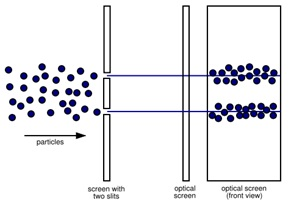
\includegraphics[scale=1]{vds}
	\caption{Verwachte resultaat dubbele spleet experiment.}
	\label{fig:vds}
\end{figure}
Wat echter werd waargenomen was een interferentiepatroon, Fig. \ref{fig:wds} en \ref{fig:ipat}, iets wat normaal gesproken wordt waargenomen bij golven. Bij een interferentiepatroon heb je afwisselend donkere en lichte lijnen. De donkere lijnen geven aan waar twee positieve of twee negatieve toppen van twee verschillende golven elkaar kruisen en zo elkaar versterken en de lichte lijnen geven aan waar een positieve en een negatieve top van twee verschillen de golven elkaar kruisen en zo elkaar op heffen.
\begin{figure}[h]
	\centering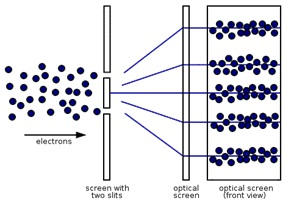
\includegraphics[scale=1]{wds}
	\caption{Waargenomen resultaat dubbele spleet experiment.}
	\label{fig:wds}
\end{figure}
\begin{figure}[h]
	\centering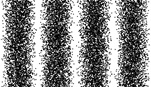
\includegraphics[scale=1]{ipat}
	\caption{Interferentiepatroon.}
	\label{fig:ipat}
\end{figure}
Bij elektronen zijn de lichte lijnen plekken waar geen elektronen zijn waargenomen en zijn de donkere lijnen plekken waar veel elektronen zijn waargenomen. Het feit dat zo’n patroon wordt waargenomen bij elektronen geeft aan dat elektronen zich soms als golven kunnen gedragen.

\subsection{Superpositie}
We hebben nu voorbeelden gezien waar golven zich als deeltjes kunnen gedragen en waar deeltjes zich als golven kunnen gedragen. Of iets zich als golf of als deeltje gaat gedragen kun je niet van tevoren weten, je ziet pas of iets een deeltje of een golf is als je het hebt gemeten. Zolang je het deeltje niet hebt gemeten zou het beiden kunnen worden en als je een systeem hebt met meerdere van dit soort deeltjes kun je niet van tevoren weten wat voor eigenschappen dat systeem gaat hebben. Wat in feite wordt gezegd is dat je niet weet wat iets is voordat je het hebt gezien. Wel is belangrijk om te melden dat het bij dit soort theorieën om de kleinste deeltjes gaat en niet om bijvoorbeeld een keukentafel. 
Zo'n nog niet gemeten deeltje kan dus van alles worden en zolang je het niet hebt gemeten is het als het ware alle mogelijke staten tegelijk. Omdat een deeltje of een golf ook nog beweegt, kan het zich mogelijk ook op andere plekken tegelijkertijd bevinden, want een deeltje beweegt zich weer anders voort dan een golf. Zo kan een deeltje, zolang hij niet gemeten is, zowel een golf als een deeltje zijn, op twee plekken tegelijkertijd zijn en wel of niet aangeslagen zijn. Als dit het geval is, is het deeltje in een superpositie. Het deeltje is dan alle mogelijke staten tegelijk en heeft het dus geen vaste eigenschappen.
Zodra het deeltje wordt gemeten "kiest" het deeltje willekeurig één van de mogelijke staten en heeft hij op dat moment dus vast te stellen eigenschappen. Maar zodra de meting klaar is, is het zeker weer mogelijk dat het deeltje weer in een superpositie raakt. Hierdoor zijn metingen van zulke systemen die zich mogelijk in een superpositie bevinden niet consistent, omdat een deeltje bij iedere meting een andere staat om in terug te vallen kan "kiezen".

\subsection{Schrödingers kat}
Een bekend gedachte-experiment wat het probleem van kwantummechanica en superposities probeert uit te leggen is Schrödingers kat. Hier wordt een kat opgesloten in een kist. In die kist bevindt zich een Geigerteller, een flesje vergif en een minuscuul radioactief deeltje, zo klein dat het binnen een uur kan vervallen maar ook helemaal niet. Als het radioactieve deeltje vervalt wordt dit gemeten door de Geigerteller, komt het vergif vrij en sterft de kat, zo niet dan leeft de kat nog. Dit radioactieve deeltje is in dit geval het deeltje wat zich in een superpositie bevindt en omdat de hele kist afhankelijk is van dit deeltje kun je zeggen dat de hele kist zich in een superpositie bevindt. Zolang je de kist niet opent weet je niet of het deeltje wel of niet is vervallen en weet je dus niet of de kat nog leeft. Zodra je de kist opent en de inhoud waarneemt kun je bepalen of de kat leeft of niet. In welke staat de superpositie terugvalt, een dode of een levende kat, als je de kist opent is willekeurig.
Het is dus onmogelijk om precies te bepalen wat of waar een deeltje in een superpositie is. Maar ondertussen is het natuurkundigen gelukt om een formule op te zetten die meest waarschijnlijke staat waarin een deeltje zal terugvallen te berekenen of eigenlijk te voorspellen. Deze voorspellende formule is de Schrödingervergelijking.

\section{Schrödingervergelijking: de theorie}
De Schrödingervergelijking is de basis van de kwantummechanica en in feite een kansberekening. De functie van de Schrödingervergelijking is om veranderingen over tijd van een fysiek systeem te berekenen en te voorspellen. Oftewel, met de Schrödingervergelijking kun je bepalen waar je een deeltje op een bepaald tijdstip kunt vinden. In de formule zitten delen waarmee je de positie ten opzichte van de $x$-as, $y$-as en $z$-as (driedimensionaal) kunt voorspellen en samen met gegevens als tijd, massa en lading van een deeltje kun je daarna ook bepalen waar het deeltje verder heen zal gaan.
Stel dat we een proef uitvoeren met een heel klein deeltje, een elektron bijvoorbeeld. In deze proef laten we een zo'n deeltje los en we observeren dan waar dat deeltje terecht komt ten opzichte van de $x$-as, de $y$-as en de $z$-as. Het rare van dit deeltje is echter dat wanneer we de proef herhalen we het deeltje op een andere plaats kunnen waarnemen. Dat is het hele eieren eten van de kwantummechanica: wanneer we kijken naar hele kleine deeltjes komen we erachter dat die deeltjes zich niet altijd gedragen zoals we verwachten. Maar dankzij de Schrödingervergelijking kunnen we een goede gok wagen op wat hun gedrag gaat worden.
\begin{figure}[h]
	\centering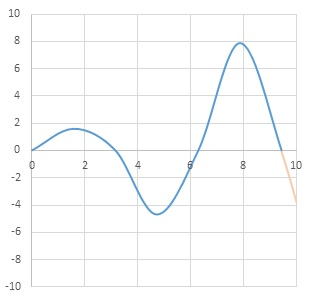
\includegraphics[scale=1]{fx5}
	\caption{$f(x)=x\cdot\sin{(x)}$.}
	\label{fig:fx5}
\end{figure}
De Schrödingervergelijking is de basis van de kwantummechanica en in feite een kansberekening. De functie van de Schrödingervergelijking is om veranderingen over tijd van een fysiek systeem te berekenen en te voorspellen. Oftewel, met de Schrödingervergelijking kun je bepalen waar je een deeltje op een bepaald tijdstip kunt vinden. In de formule zitten delen waarmee je de positie ten opzichte van de $x$-as, $y$-as en $z$-as kunt voorspellen en samen met gegevens als tijd, massa en lading van een deeltje kun je daarna ook bepalen waar het deeltje verder heen zal gaan.
Een groot deel van de berekening wordt beïnvloed door golffuncties en om een voorbeeld te geven van hoe je hier conclusies uit kunt trekken gaan we kijken naar een 'simpele versie' van de Schrödingervergelijking. Bij de simpele versie kijken we naar een tijdsonafhankelijke beweging van een deeltje langs alleen de $x$-as. Als we de Schrödingervergelijking hiertoe afleiden (wat we verderop in het hoofdstuk gaan doen) krijgen we een duidelijke golffunctie die eruit kan zien als in Fig. \ref{fig:fx5}. Dit kan een voorspelling zijn voor de als voorbeeld gegeven proef en uit deze grafiek kun je dus aflezen waar je het deeltje kunt waarnemen.
Natuurkundige Max Born kwam erachter dat je op de punten waar een piek of dal te zien was een grotere kans had om een deeltje waar te nemen. Hij stelde vast dat hoe groter de piek of het dal is, des te groter de kans is om een deeltje te vinden op de x-as rond die pieken of dalen. Verder concludeerde hij dat op de punten waar de grafiek nul is, ofwel de x-as snijdt, je geen kans hebt om een deeltje te vinden. De kans voor het vinden van zo’n deeltje wordt de "probability density" genoemd, of in het Nederlands de kansdichtheid. 
\begin{figure}[h]
	\centering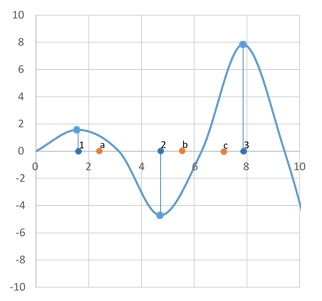
\includegraphics[scale=1]{fx6}
	\caption{$f(x)=x\cdot\sin{(x)}$ met verschillende punten.}
	\label{fig:fx6}
\end{figure}
Dit wil niet zeggen dat je op punten 1, 2 of 3 (Fig. \ref{fig:fx6}) geheid een deeltje zult vinden, want je kunt ook deeltjes tegen komen op punten a, b of c. Maar als je heel vaak een deeltje door de proefopstelling laat gaan zal je zien dat de meeste deeltjes in de buurt van punten 1, 2 en 3 worden waargenomen. De kans dat het deeltje in de buurt van 1, 2 of 3 belandt is groot, maar kans dat het deeltje op een compleet andere plek belandt is er dus nog wel. In het geval van Fig. \ref{fig:fx6} zullen de meeste deeltjes dus rond punt 3 worden waargenomen, maar er zullen ook een hoop wordt aangetroffen rond punt 2, verder zal je ook nog een aanzienlijk aantal rond punt 1 zien en de rest van losgelaten deeltjes zal verspreid zijn over de rest van de grafiek.
Als je dan op deze situaties de andere dimensies toepast en kijkt naar het tijdsverloop kunt je dus bepalen wat de meest waarschijnlijke positie van een deeltje is op het meest waarschijnlijke tijdstip en zo kun verder ook bepalen wat de meest waarschijnlijke baan van dat deeltje wordt, maar het is dus nog wel mogelijk dat het deeltje in de werkelijkheid de compleet andere kant opgaat.

\section{Schrödingervergelijking: de formule}
We gaan hier kijken naar de vergelijking zelf en onderdelen van de vergelijking uit elkaar pluizen. We gaan echter niet kijken hoe Schrödinger op de vergelijking is gekomen, omdat dat een lang en veel te moeilijk verhaal gaat worden wat verder niet veel toepassing heeft op ons onderzoek. Zoals eerder als snel genoemd werd zijn er twee versies van de Schrödingervergelijking, de tijdsafhankelijke vergelijking en de tijdsonafhankelijke vergelijking. We gaan eerst naar de tijdsafhankelijke versie kijken.

\subsection{Tijdsafhankelijke Schrödingervergelijking}
\begin{definition}[Tijdsafhankelijke Schrödingervergelijking]\label{eq:tsv}
De tijdsafhankelijke schrödingervergelijking is als volgt.
\begin{align}
i \cdot \hslash \cdot \frac{\delta}{\delta t} \cdot \Psi(r,\,t) = \hat{H} \cdot \Psi(r,\,t)
\end{align}
\end{definition}

Al meteen zijn er een hoop onbekende tekens en letters te zien. Dus laten we deze stuk voor stuk toelichten en zo duidelijk mogelijk uitleggen.
\begin{enumerate}
\item $i$ is het imaginaire getal
\item $\hslash$ is de gereduceerde constante van Planck of de constante van Dirac
\begin{enumerate}
\item $\hslash = \frac{h}{2\pi}$, waarbij $h$ de constante van Plank is
\item $h = 6,626 \cdot 10^{-34} Js$
\item $\hslash = 1,054 \cdot 10^{-34}$
\item de eenheid $Js$ is joule maal seconde en geeft het verband tussen de energie en frequentie van een deeltje aan
\end{enumerate}
\item $\frac{\delta}{\delta t}$ is de afgeleide van de tijd $t$ en geeft het tijdsverloop aan
\item $\Psi(r,\,t)$ is de golffunctie en eigenlijk de oplossing voor vergelijking
\begin{enumerate}
\item $r$ geeft de coördinaten van het deeltje (dit kunnen cartesische coördinaten zijn maar ook poolcoördinaten)
\item $t$ geeft de tijd behorende bij $r$ aan
\item $\Psi(r,\,t)=\psi(r)\cdot e^{-i\frac{E}{\hslash}t}=\psi(r)\cdot e^{-2\pi i\frac{E}{h}t}$
\begin{enumerate}
\item $\psi(r)$ geeft de beweging ten opzichte van de coördinaten
\item $e^{-2\pi i\frac{E}{h}t}$ geeft tijdsafhankelijke deel weer en E is hier de totale energie van het deeltje in Joule
\end{enumerate}
\end{enumerate}
\item $\hat{H}$ is een Hamiltoniaan, waarvoor de formule $\hat{H}=\hat{T}+\hat{V}$ gebruikt wordt
\begin{enumerate}
\item $\hat{V}$ is de potentiele energie van een deeltje in een systeem met betrekking op de plaats van het deeltje en moment van de meting en schrijven we daarom als $V(r,\,t)$
\item $\hat{T}$ is de kinetische energie in een systeem en bereken je als $\hat{T} = \frac{\hat{p}^2}{2m}$
\begin{enumerate}
\item $m$ = is de massa van een deeltje in kilogram
\item $\hat{p}$ is de impulsoperator en geeft de relatie tussen de snelheid en de massa van een deeltje in de kwantum mechanica. De impulsoperator wordt berekend als $\hat{p}=-i\hslash\nabla$
\begin{enumerate}
\item $\nabla$ is een nabla en is geeft de beweging van een deeltje aan. Als je cartesische coördinaten gebruikt schrijf je het als $\nabla = \frac{\delta}{\delta x}+\frac{\delta}{\delta y}+\frac{\delta}{\delta z}$, maar wordt voor het overzicht $\nabla$
\end{enumerate}
\end{enumerate}
\end{enumerate}
\end{enumerate}
Dus
\begin{align*}
\hat{T} &= \frac{\hat{p}^2}{2m}\\
&=\frac{(-i\hslash)^2}{2m}\cdot \nabla^2\\
&=-\frac{\hslash^2}{2m}\cdot \left(\frac{\delta^2}{\delta x^2}+\frac{\delta^2}{\delta y^2}+\frac{\delta^2}{\delta z^2}\right)\\
&= -\frac{\frac{h^2}{4\pi^2}}{2m}\cdot\left(\frac{\delta^2}{\delta x^2}+\frac{\delta^2}{\delta y^2}+\frac{\delta^2}{\delta z^2}\right)\\
&= -\frac{h^2}{8\pi^2m}\cdot\left(\frac{\delta^2}{\delta x^2}+\frac{\delta^2}{\delta y^2}+\frac{\delta^2}{\delta z^2}\right)
\end{align*}
en
\begin{align*}
\hat{H} &=-\frac{h^2}{8\pi^2m}\cdot\left(\frac{\delta^2}{\delta x^2}+\frac{\delta^2}{\delta y^2}+\frac{\delta^2}{\delta z^2}\right)+V(r,\,t).
\end{align*}

Als we de tijdsafhankelijke Schrödingervergelijking dan uitgebreid willen schrijven krijgen we het volgende.
\begin{displaymath}
\frac{ih}{2\pi}\cdot\frac{\delta}{\delta t}\cdot \left(\psi(r)\cdot e^{-2\pi i\frac{E}{h}t}\right) = \left(-\frac{h^2}{8\pi^2m}\cdot\left(\frac{\delta^2}{\delta x^2}+\frac{\delta^2}{\delta y^2}+\frac{\delta^2}{\delta z^2}\right)+V(r,\,t)\right)\cdot\left(\psi(r)\cdot e^{-2\pi i \frac{E}{h}t}\right)
\end{displaymath}
Zoals je kunt zien aan imaginaire getallen die in de Schrödingervergelijking staan is dit dus een complexe vergelijking.\cite{wiki:schr}\cite{wiki:ham}

\subsection{Tijdsonafhankelijke Schrödingervergelijking}
\begin{displaymath}
\hat{H}\cdot \Psi(r)=E\cdot \Psi(r)
\end{displaymath}
Hier worden over het algemeen dezelfde tekens en letters gebruikt, maar ze zijn net even anders.
\begin{enumerate}
\item $\hat{H}$ is bij de tijdsonafhankelijke Schrödingervergelijking $\hat{H}=-\frac{h^2}{8\pi^2m}\cdot \left(\frac{\delta^2}{\delta x^2}+\frac{\delta^2}{\delta y^2}+\frac{\delta^2}{\delta z^2}\right)+V(r)$
\begin{enumerate}
\item Het is hier $V(r)$ i.p.v. $V(r,\,t)$ omdat we nu geen focus meer leggen op het tijdsverloop van de metingen
\end{enumerate}
\item De golffunctie is hier $\Psi(r)$ in plaats van $\Psi(r,\,t)$ omdat we ook hier niet kijken naar het tijdsverloop en schrijven voor de golffunctie $\psi(r)$ en we laten $e^{-2\pi i\frac{E}{h}t}$ weg omdat dit van toepassing is op de tijd en daar wordt bij deze versie van de Schrödingervergelijking niet mee gerekend
\item E is ook hier de totale energie van het deeltje.
\end{enumerate}

De uitgewerkte tijdsonafhankelijke Schrödingervergelijking ziet er als volgt uit.
\begin{displaymath}
\left(-\frac{h^2}{8\pi^2m}\cdot \left(\frac{\delta^2}{\delta x^2}+\frac{\delta^2}{\delta y^2}+\frac{\delta^2}{\delta z^2}\right)+V(r)\right)\cdot \psi(r)=E\cdot \psi(r)
\end{displaymath}

Ook al zie je in de uitgewerkte versie geen imaginair getal is dit nog steeds een complexe vergelijking, want in de impulsoperator die in de Hamiltoniaan verwerkt is staat namelijk een imaginair getal. Het moet dus wel een complexe vergelijking zijn want met een reële getallenverzameling zou je op een andere vergelijking uitkomen.

De oplossing voor beide vergelijking is de kansdichtheid. Natuurkundige Max Born kwam erachter dat je deze kansdichtheid kunt berekenen door de absolute waarde van de golffunctie te kwadrateren, dit geeft ${\left|\Psi\right|}^2$. De tijdsonafhankelijke vergelijking wordt ${\left|\Psi\right|}^2=\left|{\psi(r)}^2\right|$. Bij de tijdsafhankelijke vergelijking wordt het het volgende\cite{maf}.
\begin{align}\label{eq:psipsi}
{\left|\Psi(r,\,t)\right|}^2 &=\left|{\psi(r)}^2\cdot e^{-2(2\pi i \frac{E}{h})t}\right|\nonumber\\
&=\left|{\psi(r)}^2\right|\cdot\left|e^{-2(2\pi i\frac{E}{h})t}\right|\nonumber\\
&=\left|{\psi(r)}^2\right|,
\end{align}
want
\begin{displaymath}
e^{-2(2\pi i \frac{E}{h})t}=\cos{\left(-2\left(\frac{2\pi E}{h}\right)t\right)}+i\sin{\left(-2\left(\frac{2\pi E}{h}\right)t\right)}.
\end{displaymath}
Dit geeft
\begin{displaymath}
\left|\cos{\left(-2\left(2\pi\frac{E}{h}\right)t\right)}+i\sin{\left(-2\left(2\pi\frac{E}{h}\right)t\right)}\right|=\cos^2{\left(-2\left(2\pi\frac{E}{h}\right)t\right)}+\sin^2{\left(-2\left(2\pi\frac{E}{h}\right)t\right)}=1,
\end{displaymath}
want
\begin{displaymath}
\cos^2{\left(A\right)}+\sin^2{\left(A\right)}=1
\end{displaymath}

\section{De Schrödingervergelijking in actie}
We gaan nu kijken naar een voorbeeld van de Schrödingervergelijking. Om het simpel te houden gaan we kijken naar een tijdsonafhankelijk eendimensionaal voorbeeld. Een voordeel hiervan is dat de golffunctie in alleen dit geval een simpele sinus-cosinus functie is, wat niet het geval zou zijn in een twee- of driedimensionaal voorbeeld.
\begin{figure}[h]
	\centering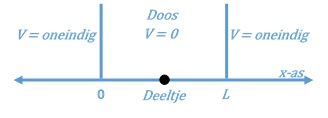
\includegraphics[scale=1]{tes}
	\caption{Schematische weergave van de doos.}
	\label{fig:tes}
\end{figure}
Voor dit voorbeeld nemen we een deeltje dat in een doos tussen twee ondoordringbare muren stuitert en het deeltje beweegt alleen heen weer langs de $x$-as, zie Fig. \ref{fig:tes}. De ondoordringbare muren staan op $x = 0$ en $x = L$.  Omdat er binnen de doos zijn er geen krachten of andere voorwerpen die het deeltje binnen de doos beïnvloeden is de potentiële energie $V$ op het deeltje binnen de doos is nul. Dus $V(x)=0$ bij $0 < x < L$. Als het deeltje bij de muren komt wordt het deeltje met een oneindig grote kracht de andere kant opgeduwd, want de muren zijn ondoordringbaar en de energie van het deeltje kan dus nooit groot genoeg zijn om door de muren te komen. De potentiële energie op het deeltje is dan oneindig groot wanneer het deeltje tegen de muur aankomt en de andere kant op wordt geduwd. Dus $V(x)=\infty$ bij $x\leq 0$ en $x\geq L$. Nu we dit weten kunnen de Schrödingervergelijking erbij halen en de tijdsonafhankelijke eendimensionale Schrödingervergelijking ziet er als volgt uit.
\begin{displaymath}
-\frac{h^2}{8\pi^2m}\cdot\frac{\delta^2\cdot \psi(x)}{\delta x^2}+V(x)\cdot \psi(x)=E\cdot\psi(x)
\end{displaymath}
$m$ is de massa van het deeltje, $E$ is de totale energie en de constante van Planck $h=6,626068\cdot10^{-34} Js$. Om verder te kunnen werken met de vergelijking moeten we $V(x)\cdot\psi(x)$ aan de rechterkant van de vergelijking krijgen en de rest van aan linker kant. Dit doen we als volgt.
\begin{align*}
-\frac{h^2}{8\pi^2m}\text{naar de rechterkant delen geeft}\\
\frac{\delta^2\cdot\psi(x)}{\delta x^2}+V(x)\cdot\psi(x) &= \frac{E\cdot\psi(x)}{-\frac{h^2}{8\pi^2m}}\\
&= -\frac{8\pi^2\cdot m\cdot E\cdot\psi(x)}{h^2}\\
-\frac{8\pi^2\cdot m\cdot E\cdot\psi(x)}{h^2}\text{naar de linker kant halen geeft}\\
\frac{\delta^2\cdot\psi(x)}{\delta x^2}+\frac{8\pi^2\cdot m\cdot E\cdot\psi(x)}{h^2}+V(x)\cdot\psi(x) &= 0\\
V(x)\cdot\psi(x)\text{naar de rechter kant halen geeft}\\
\frac{\delta^2\cdot\psi(x)}{\delta x^2}+\frac{8\pi^2\cdot m\cdot E\cdot\psi(x)}{h^2} &= V(x)\cdot\psi(x)\\
\end{align*}

Wanneer we de locatie van het deeltje binnen de doos willen weten is $V(x)=0$ en dan krijgen we:
\begin{displaymath}
\frac{\delta^2\cdot\psi(x)}{\delta x^2}+\frac{8\pi^2\cdot m\cdot E\cdot\psi(x)}{h^2} = 0
\end{displaymath}
Om de vergelijking op te lossen moeten we achter $\psi(x)$ komen. Als we de vergelijking als functie van $\psi(x)$ schrijven krijgen we het volgende.
\begin{displaymath}
\psi(x)=A\cdot \cos{\left(\sqrt{\frac{8\pi^2\cdot m\cdot E}{h^2}}\cdot x\right)}+B\cdot\sin{\left(\sqrt{\frac{8\pi^2\cdot m\cdot E}{h^2}}\cdot x\right)}
\end{displaymath}
$A$ en $B$ zijn hier constanten. We weten dat $\left|{\psi(x)}^2\right|$ aangeeft wat de kans is dat het deeltje op positie x is. Verder weten we dat het deeltje nooit buiten de doos kan zijn, oftewel op $x<0$ en $x>L$, omdat de energie die het deeltje nodig zou hebben om daar te komen oneindig groot zou moeten zijn. Ook kunnen we zeggen dat het deeltje niet in de muur kan komen, oftewel op $x=0$ en $x=L$, want de muren zijn ondoordringbaar. Omdat de kans dus nul is dat het deeltje in de muren om buiten de doos is kunnen we zeggen dat $\left|{\psi(x)}^2\right| = 0$ en dus $\psi(x)=0$ bij $x<0$ en $x>L$ en bij $x=0$ en $x=L$.

De eerste situatie, $\psi=0$ bij $x=0$, geeft
\begin{align*}
\psi(0) = 0 &= A\cdot\cos{\left(\sqrt{\frac{8\pi^2\cdot m\cdot E}{h^2}}\cdot 0\right)}+B\cdot\sin{\left(\sqrt{\frac{8\pi^2\cdot m\cdot E}{h^2}}\cdot 0\right)}\\
& = A\cdot\cos{(0)}+B\cdot\sin{(0)}\\
&= A\cdot 1+B\cdot 0\\
&= A
\end{align*}
Omdat $A=0$ kunnen we onze vergelijking als volgt schrijven.
\begin{align}\label{eq:psib}
\psi(x)=B\cdot\sin{\left(\sqrt{\frac{8\pi^2\cdot m\cdot E}{h^2}}\cdot x\right)}
\end{align}
De tweede situatie is, $\psi=0 $bij $x=L$, geeft:
\begin{displaymath}
\psi(0)=B\cdot\sin{\left(\sqrt{\frac{8\pi^2\cdot m\cdot E}{h^2}}\cdot L\right)}=0
\end{displaymath}
Dit betekent dat $B=0$ of dat de sinus gelijk is aan nul. Als $B=0$ zouden we niks aan onze vergelijking hebben, want dan is onze vergelijking overal nul. Dit zou betekenen dat de kansdichtheid overal nul is en dat ons deeltje dus nergens is, maar we weten dat het deeltje in de doos is dus dit is niet mogelijk. Dit betekent dus dat de sinus gelijk is aan nul.
\begin{displaymath}
\sin{\left(\sqrt{\frac{8\pi^2\cdot m\cdot E}{h^2}}\cdot L\right)}
\end{displaymath}
Wanneer $\sin{(x)}=0$ dan $x=\{0, \pi, 2\pi, 3\pi,\ldots\} $ oftewel $x = n\pi$. Dan kunnen we dus zeggen dat
\begin{displaymath}
\sqrt{\frac{8\pi^2\cdot m\cdot E}{h^2}}\cdot L=n\cdot \pi
\end{displaymath}
Om verder te kunnen rekenen moeten we de totale energie $E$ uit de vergelijking los maken.
Eerst delen we $L$ naar de rechterkant.
\begin{displaymath}
\sqrt{\frac{8\pi^2\cdot m\cdot E}{h^2}}=\frac{n\cdot \pi}{L}
\end{displaymath}
Dan kwadrateren we de wortel weg.
\begin{displaymath}
\frac{8\pi^2\cdot m\cdot E}{h^2}=\frac{n^2\cdot \pi^2}{L^2}
\end{displaymath}
Dan vermenigvuldigen we $h^2$ naar de rechterkant.
\begin{displaymath}
8\pi^2\cdot m\cdot E=\frac{n^2\cdot\pi^2\cdot h^2}{L^2}
\end{displaymath}
Daarna delen we $8\pi^2*m$ naar de rechterkant.
\begin{align*}
E_n &= \frac{n^2\cdot\pi^2\cdot h^2}{L^2\cdot 8\pi^2\cdot m}\\
&= \frac{n^2\cdot h^2}{8\cdot m\cdot L^2}
\end{align*}
Hier geldt $n=\{0, 1, 2, 3, \ldots\}$ Dit betekent dat $E_n$, het energieniveau van het deeltje, omhoog gaat met duidelijke stappen. Als $n=0$ zou het betekenen dan $\psi=0$ overal in de doos, wat zou betekenen dat het deeltje niet in de doos is, maar dit kan niet want we weten zeker dat het deeltje in de doos is. Dus eigenlijk geldt $n=\{0, 1, 2, 3, \ldots\}$ voor $E_n$.

We moeten nu eerst een stap maken naar de eerder besproken kansdichtheid berekening. We hebben Vgl. \ref{eq:psipsi} al eerder vastgesteld.
Om hier een kansberekening uit te krijgen moeten we de integraal hiervan nemen.
\begin{displaymath}
\int_0^L {\left|\Psi(x)\right|}^2\,dx=\int_0^L \left|{\psi(x)}^2\right|\,dx
\end{displaymath}
Deze integraal geeft de kans dat het deeltje tussen twee waardes van $x$ is en omdat we weten dat het deeltje zeker tussen $x=0$ en $x=L$ is, kunnen we stellen dat
\begin{displaymath}
\int_0^L {\left|\Psi(x)\right|}^2\,dx=\int_0^L \left|{\psi(x)}^2\right|\,dx=1
\end{displaymath}
Als we dan nu voor $\psi(x)$ invullen wat we eerder daaraan hebben gelijkgesteld, zie Vgl. \ref{eq:psib}, krijgen we het volgende.
\begin{displaymath}
\int_0^L B^2\cdot\sin^2{\left(\sqrt{\frac{8\pi^2\cdot m\cdot E}{h^2}}\cdot x\right)}\,dx=1
\end{displaymath}
We kunnen deze functie verder uitwerken als we de volgende regel weten.
\begin{displaymath}
\int \sin^2{(ax)}\,dx=-\frac{1}{2a}\sin{(ax)}+\frac{x}{2}
\end{displaymath}

Als we dit gebruiken krijgen we de volgende berekening.
\begin{align*}
&\int_0^L B^2\sin^2{\left(\sqrt{\frac{8\pi^2\cdot m\cdot E}{h^2}}\cdot x\right)}\,dx\\
&= \left[-\frac{B^2}{2\sqrt{\frac{8\pi^2\cdot m\cdot E}{h^2}}}\cdot\sin{\left(\sqrt{\frac{8\pi^2\cdot m\cdot E}{h^2}}\cdot x\right)}\cdot\cos{\left(\sqrt{\frac{8\pi^2\cdot m\cdot E}{h^2}}\cdot x\right)}+\frac{B^2\cdot x}{2}\right]_0^L\\
&=\left(-\frac{B^2}{2\sqrt{\frac{8\pi^2\cdot m\cdot E}{h^2}}}\cdot\sin{\left(\sqrt{\frac{8\pi^2\cdot m\cdot E}{h^2}}\cdot L\right)}\cdot\cos{\left(\sqrt{\frac{8\pi^2\cdot m\cdot E}{h^2}}\cdot L\right)}+\frac{B^2\cdot L}{2}\right)\\
&- \left(-\frac{B^2}{2\sqrt{\frac{8\pi^2\cdot m\cdot E}{h^2}}}\cdot\sin{\left(\sqrt{\frac{8\pi^2\cdot m\cdot E}{h^2}}\cdot 0\right)}\cdot\cos{\left(\sqrt{\frac{8\pi^2\cdot m\cdot E}{h^2}}\cdot 0\right)}+\frac{B^2\cdot 0}{2}\right)\\
&= 1
\end{align*}
We weten dat
\begin{displaymath}
\sin{\left(\sqrt{\frac{8\pi^2\cdot m\cdot E}{h^2}}\cdot L\right)}=0
\end{displaymath}
en dat
\begin{displaymath}
\sin{\left(\sqrt{\frac{8\pi^2\cdot m\cdot 0}{h^2}}\cdot L\right)}=0
\end{displaymath}
We kunnen de vergelijking nu als volgt schrijven.
\begin{align*}
&-\frac{B^2}{2\sqrt{\frac{8\pi^2\cdot m\cdot E}{h^2}}}\cdot 0\cdot\cos{\left(\sqrt{\frac{8\pi^2\cdot m\cdot E}{h^2}}\cdot L\right)}+\frac{B^2\cdot L}{2}+\frac{B^2}{2\sqrt{\frac{8\pi^2\cdot m\cdot E}{h^2}}}\cdot 0\cdot 1+0\\
&= 0+\frac{B^2\cdot L}{2}+0\\
&= \frac{B^2\cdot L}{2}\\
&= 1
\end{align*}
We hebben nu de kans om hier een vergelijking voor $B$ uit af te leiden.
\begin{align*}
\frac{B^2\cdot L}{2} &=1\\
B^2 &=\frac{2}{L}\\
B = \sqrt{\frac{2}{L}} &\vee B = -\sqrt{\frac{2}{L}}\\
\text{vold.} &\quad \text{vold. niet}
\end{align*}
Als we nu onze $B$ in onze vergelijking voor $\psi(x)$ substitueren krijgen we het volgende.
\begin{displaymath}
\psi(x)=\sqrt{\frac{2}{L}}\cdot\sin{\left(\sqrt{\frac{8\pi^2\cdot m\cdot E}{h^2}}\cdot x\right)}
\end{displaymath}
Verder kunnen we hier ook de vergelijking voor $E$ die we eerder hadden gevonden in substitueren.
\begin{align*}
\psi_n(x) &=\sqrt{\frac{2}{L}}\cdot\sin{\left(\sqrt{\frac{8\pi^2\cdot m\cdot \frac{n^2\cdot h^2}{8\cdot m\cdot L^2}}{h^2}}\cdot x\right)}\\
&= \sqrt{\frac{2}{L}}\cdot\sin{\left(\sqrt{\frac{8\pi^2\cdot m\cdot n^2\cdot h^2}{h^2\cdot 8\cdot m\cdot L^2}}\cdot x\right)}\\
&= \sqrt{\frac{2}{L}}\cdot\sin{\left(\sqrt{\frac{\pi^2\cdot n^2}{L^2}}\cdot x\right)}\\
&= \sqrt{\frac{2}{L}}\cdot\sin{\left(\frac{\pi\cdot n\cdot x}{L}\right)}\quad \text{bij } 0<x<L
\end{align*}
Voor elke andere $x$ geldt $\psi_n(x)=0$.

We zien hier verder een ander opvallend resultaat. Voor elke waarde van n die groter is dan 1 is er een waarde van x binnen de doos waarvoor geldt
\begin{displaymath}
{\left|\Psi(x)\right|}^2=\left|{\psi(x)}^2\right|=0,
\end{displaymath}
dus het is onmogelijk dat het deeltje dan op die waarde van $x$ is. Voor deze waardes van $x$ geldt
\begin{displaymath}
x=\frac{k\cdot L}{n}
\end{displaymath}
Voor $k$ geldt $k=\{1, 2, 3, \ldots\}$ en $k<n$. Dus als voorbeeld, als $n=5$, dan geldt $k=4$. Voor deze waardes van $x$ kunnen we een speciale versie van de vergelijking voor $\psi_n(x)$ schrijven.
\begin{align*}
\psi_n(x) &= \sqrt{\frac{2}{L}}\cdot\sin{\left(\frac{\pi\cdot n\cdot \frac{k\cdot L}{n}}{L}\right)}\\
&= \sqrt{\frac{2}{L}}\cdot\sin{\left(\frac{\pi\cdot n\cdot k\cdot L}{L\cdot n}\right)}\\
&= \sqrt{\frac{2}{L}}\cdot\sin{\left(\pi\cdot k\right)}
\end{align*}
Want elke waarde van $\sin{(x)}$ is gelijk aan 0 als er voor $x$ geldt $x=\{0, \pi, 2\pi, 3\pi, \ldots\}$.

\chapter{Kijken naar het oneindige}
Het heelal bestaat uit miljarden sterrenstelsel, die sterrenstelsels bestaan ook weer uit miljoenen sterren en om die sterren draaien weer een miljoen verschillende planeten. De grootte van het heelal is niet voor te stellen, maar toch is het wetenschappers gelukt om een theorie te bedenken over hoe alles begon en hoe alles wat er in het heelal is er zo gevormd is. Denk maar eens aan hoe een sterrenstelsel er uit ziet. Zoek eens op google naar plaatjes ervan en je ziet dat bijna alle sterrenstelsels een gelijkenis hebben in hun vorm. Maar het is niet zomaar een vorm, het is een fractal. Door aan te nemen dat sterrenstelsels in fractale vormen zijn opgebouwd werden er nieuwe ontdekkingen gedaan over het bestaan van het heelal door simpel terug te rekenen, maar hoe zit dat eigenlijk? Wat is de toepassing van een Fractal en wat heeft het complexe vlak daar mee te maken?

\section{Fractals}
Fractals zijn oneindige zichzelf herhalende patronen. Als je eenmaal weet hoe deze eruit zien, herken je fractals overal om je heen. 
Neem nou een boom. Zo bestaat een boom uit een stam met takken, takken met zijtakken, zijtakken met twijgen en twijgen met naalden.
\begin{figure}[h]
	\centering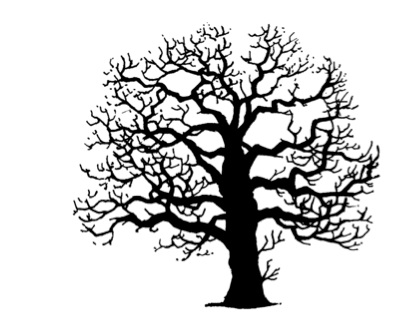
\includegraphics[scale=1]{boom}
	\caption{Een boom.}
	\label{fig:boom}
\end{figure}
Of wat denk je van de bliksem, de grote bliksemschicht krijgt allemaal vertakkingen naar kleinere bliksemschichtjes.
\begin{figure}[h]
	\centering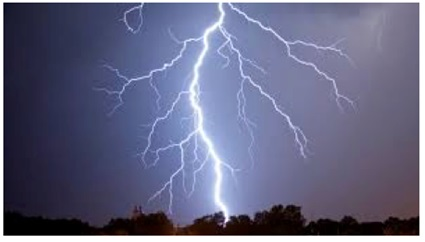
\includegraphics[scale=1]{blisem}
	\caption{Een bliksemschicht.}
	\label{fig:bliksem}
\end{figure}

Fractals komen overal in de natuur voor. Van de grootste sterrenstelsels in het heelal tot de kleinste planten op aarde, overal lijken kleinere structuren op grotere structuren. Maar fractals kunnen ook worden gebruikt in computermodellen, om zo bijvoorbeeld meer te leren over het ontstaan van sterrenstelsels die met behulp van simulaties kunnen worden uitgevoerd. Of fractals kunnen gebruikt worden door een computer om grote bestanden te doorzoeken. Een iets minder wetenschappelijke toepassing maar wel echt actueel van fractals is de toepassing in computerspellen. Het is een stuk gemakkelijker om een object van een fractal te maken, die tijdens het inzoomen gedetailleerder wordt, dan dat een object pixel voor pixel opgebouwd moet worden. Kortom: fractals zijn overal. Echter: eenvoudig is een fractal niet, dus laten we beginnen bij het begin.

\section{Informatie vooraf}
Goed verankerde basiskennis van wiskunde is een voorwaarde om met wiskunde op een hoger niveau te kunnen werken. Dat kan door oefenen, oefenen en nog eens oefenen. Wiskunde is een proces van toepassen van wat je al weet in iets nieuws. Je inzoomen op deze voorkennis van vormen, processen, wetmatigheden en structuren geeft inzicht en begrip. Kortom: Wiskunde leren is fractal. 
Voordat we ons gaan verdiepen in de diepe troggen van de wiskunde van fractals moeten we ons eerst bewust zijn van wat er allemaal vooraf gebeurt bij het maken van een fractal. 
\begin{figure}[h]
	\centering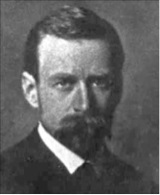
\includegraphics[scale=1]{koch}
	\caption{Helge von Koch.}
	\label{fig:koch}
\end{figure}
We nemen als voorbeeld de Koch Snowflake. De Zweedse wiskundige Helge von Koch maakte in 1904 de zogenaamde KochCurve door uit elk driehoeksbeen het midden uit te halen en daar weer een driehoek neer te zetten, zie Fig. \ref{fig:drie}. De sneeuwvlok die ontstaat door wiskunde figuren eindeloos volgens eenzelfde patroon te vermenigvuldigen. Neem de gelijkbenige driehoek. 
\begin{figure}[h]
	\centering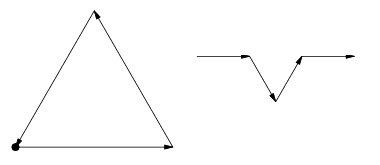
\includegraphics[scale=1]{drie}
	\caption{Driehoeken in driehoeken.}
	\label{fig:drie}
\end{figure}
\begin{figure}[h]
	\centering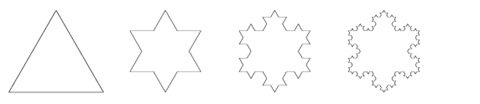
\includegraphics[scale=1]{vlok}
	\caption{Een sneeuwvlok.}
	\label{fig:vlok}
\end{figure}

De wiskundige formule is eigenlijk heel eenvoudig. Je gaat uit van: 
\begin{enumerate}
\item Eén zijde van een driehoek, wordt omgevormd tot 4 zijden, Fig. \ref{fig:drie}
\item Een driehoek heeft drie zijden die allen omgevormd worden tot 4 zijden, Fig. \ref{fig:vlok}. 
\item Dit herhaalt zich dus.....eindeloos.
\end{enumerate}
Wiskundig geformuleerd:
\begin{enumerate}
\item $3\cdot 4^1=12$
\item $3\cdot 4^2=48$
\item $3\cdot 4^n=\ldots$
\end{enumerate}
De $n$ in de formule wordt na verloop van tijd $\infty$: $3\cdot 4^\infty=\infty$.

Hier boven is een proces beschreven wat eindeloos door kan blijven gaan. Elke driehoek kan weer opsplitsen in nog meer driehoeken. Uiteindelijk worden de driehoeken zo klein dat ze niet meer te zien zijn met het blote oog. Dit is een van de makkelijkste vormen van een fractal, maar het laat goed zien hoe eindeloos een fractal eigenlijk wel niet is.
Om de fractals te begrijpen waarbij meer komt kijken dan het voorbeeld hierboven (bijvoorbeeld het complexe vlak) duiken we nog dieper in de theorie van de fractals.

\section{Aangetrokken worden door wiskunde}
\begin{figure}[h]
	\centering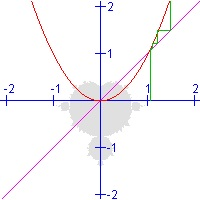
\includegraphics[scale=1]{fx7}
	\caption{De functie $y=x^2$.}
	\label{fig:fx7}
\end{figure}
De grafiek in Fig. \ref{fig:fx7} laat een dal parabool zien die het minimum als oorsprong heeft. Om van deze functie de y waarde te kunnen berekenen gaat er in principe niet veel spannends gebeuren. Laten we het getal 2 nemen. Daarvan nemen we het kwadraat. Dat is 4, maar als we daar weer het kwadraat van nemen en daarna weer, dan kom je eerst uit op 16 dan 256, 65536 en ga zo maar door. Totdat de rekenmachine zegt error. Het getal dat uit het voortschrijdende kwadrateren komt wordt te groot voor de rekenmachine om aan te geven. Dit proces noemen we itereren en zal nog veel terugkomen bij het maken van een fractal. Nemen we het getal 1,01 of 1,4 dan gaat het proces van itereren een stuk langzamer, als je kijkt naar de grootte van het getal dat er steeds uitkomt na het kwadrateren. Als het een getal is boven de 1 (dus zelfs 1,00000001) gaat het itereren uiteindelijk naar oneindig. Kijken we naar de getallen die kleiner zijn dan 1 bijvoorbeeld 0,5 ligt dat anders. Het kwadraat van 0,5 is namelijk 0,25 en daarvan het kwadraat is 0,0625. Dit gaat in de richting van de nul.

Nu hebben alle getallen die groter of kleiner zijn dan 1 een eindstation waar ze uiteindelijk heen gaan namelijk: naar oneindig of naar 0, maar hoe zit het dan met 1? De 1 blijft keurig op zijn plek staan, als je 1 namelijk kwadrateert krijg je 1, hoe vaak je ook blijft kwadrateren. De 1 is dus een scheiding van de getallen die naar 0 gaan (worden aangetrokken) en de getallen die naar oneindig gaan. Het punt 0 noemen we een aantrekker. Dit geldt ook voor de negatieve getallen, want getallen groter dan –1 gaan naar nul en getallen kleiner dan -1 gaan naar (min)oneindig. Als we dus even terugkomen op de parabool, Fig. \ref{fig:fx9} heeft de parabool een aantrekker in het punt $x=0$, voor de start waarde tussen -1 en 1. De groene lijn geeft de weg van het aantrekkingspunt weer.
\begin{figure}[h]
	\centering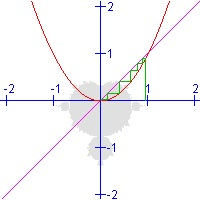
\includegraphics[scale=1]{fx9}
	\caption{De functie $y=x^2$.}
	\label{fig:fx9}
\end{figure}
Met deze informatie zijn we al een heel stuk op weg, maar met deze toepassingen blijven we met het aantrekkingspunt 0 en zal er dus nooit een mooi groot fractal figuur uitkomen. Daarom moeten we ervoor zorgen dat de parabool waar we het hierboven over hadden moet kunnen worden verplaats. De parabool verticaal verplaatsen doen we door er een $c$ bij toe te voegen. De formule wordt dan $y=x^2+c$. Het minimum van de parabool is dan $c$, elk cijfer wat er als c wordt gebruikt staat gelijk aan het minimum van de parabool. Als we dan teruggaan naar het begrip itereren en die toepassing uitvoeren zien we dat er nog steeds een aantrekkingspunt is alleen dat is niet meer 0, er is een ander aantrekkingspunt is gekomen, Fig. \ref{fig:fx10}.
\begin{figure}[h]
	\centering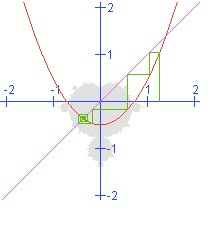
\includegraphics[scale=1]{fx10}
	\caption{De functie $y=x^2+c$ met $c=-0,5$.}
	\label{fig:fx10}
\end{figure}
We zien in Fig. \ref{fig:fx10} nu weer een aantrekker alleen is de aantrekker niet nul. De aantrekker is precies het snijpunt van de parabool met de diagonaal. Het andere snijpunt die te zien is in het figuur heeft ook een functie namelijk wanneer de startwaarde bij een iteratie, een getal is die rechts van het snijpunt ligt, gaat die naar oneindig. Voor de snijpunten geldt hiervoor ook de volgende formule $y=x^2+c$ met nog steeds $c=-0,5$, als we die tegen de formule van de parabool zetten krijgen we daar snijpunten uit namelijk: -0,366 en 1,366
Met alles even op een rijtje voor de formule van $y=x^+c$ met als $c= -0,5$ worden alle getallen met als start waarden tussen -1,366 en 1,366 aangetrokken door het punt -0,366.

\begin{figure}[h]
	\centering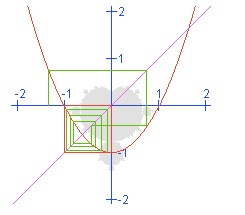
\includegraphics[scale=1]{fx8}
	\caption{De functie $y=x^2+c$ met $c=-1$.}
	\label{fig:fx8}
\end{figure}
We bekijken een volgend geval: $c =-1$, Fig. \ref{fig:fx8}.
Uit figuur 6 blijkt iets opmerkelijks: de startwaarde gaat bij itereren niet naar een vast punt toe, maar blijft heen en weer springen, in dit geval tussen de waarden 0 en -1 (rood aangegeven). We noemen dit een dubbele aantrekker. De getallen zijn eenvoudig na te rekenen Neem als startwaarde 0. Als we die staartwaarde invullen in de parabool geeft de eerste iteratie: -1. Vullen we die waarde opnieuw in, dan vinden we als tweede iteratie 0. Bij andere startwaarden worden de getallen al moeilijker en kan het wat langer duren, maar ook dan kom je uit op dezelfde dubbele aantrekker.

Nu begint het pas echt interessant te worden en komen we dichter bij het begrijpen van een fractal. Als we de formules van hierboven nog eens bekijken en met name $y=x^2+c$ zijn er wat opmerkelijke aspecten die we tegen komen, namelijk: als we de c kleiner maken dan -2 of groter dan 0.25, is er geen aantrekker, elke startwaarde gaat bij itereren naar oneindig. 
Als we een c nemen tussen -0,75 en 0,25 is er een enkelvoudige aantrekker.
Een nog interessanter fenomeen is als we de c nog meer verlagen dan -1,25 er een vierdubbele aantrekker komt en als we nog iets kleiner gaan er een klein gebiedje komt met een achtdubbele aantrekker, dat is bijvoorbeeld bij $c=-1,39$. Maken we de c nog iets negatiever, dan stopt deze zogenaamde periodeverdubbeling en gebeurt er iets heel merkwaardigs. Er is namelijk wel een gebied van startwaarden dat wordt aangetrokken, maar het itereren gaat niet naar een aanwijsbare of meervoudige aantrekker toe. Er is geen enkele regelmaat meer te herkennen in hoe de aantrekker zich gedraagt. We noemen dit chaotisch gedrag. De aantrekker die er niet maar toch ook weer wel is, noemen we een Vreemde Aantrekker. Rond dit chaotisch gedrag heeft zich een geheel nieuwe wetenschappelijke studie ontwikkeld namelijk de Chaostheorie hier komen we later nog op terug.

\begin{figure}[h]
	\centering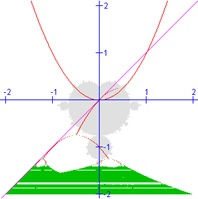
\includegraphics[scale=1]{fx11}
	\caption{De functie $y=x^2$ met vertakkingen.}
	\label{fig:fx11}
\end{figure}
Deze opmerkelijke fenomenen zijn allemaal samengevat in Fig. \ref{fig:fx11}. Een korte toelichting aan dit toch wel merkwaardige figuur. Voor elke waarde van $c$ zijn de aantrekkers als rode of groene punten aangegeven op een horizontale lijn door $c$. Bijvoorbeeld voor $c = -1.00$ is er een dubbele aantrekker gevonden: 0 en -1. Trekken we een horizontale lijn door het punt $y = -1$ dan zie je dat die inderdaad de boom snijdt in de punten 0 en -1. 
Trek je de horizontale lijn wat lager, dan passeer je een vertakking en krijg je vier snijpunten en zo zijn er nog veel meer snijpunten.
Wat dieper begint de chaos: de hele lijn is groen. 
De groene waas in het figuur wordt de vertakkingsboom van Feigenbaum genoemd. De vertakking is vernoemd naar de Amerikaanse wiskundige Mitchell Feigenbaum, die rond 1975 onderzoek deed op dit gebied. Als je het plaatsje omkeert lijkt het wel een beetje op een boom, daarom ook de vertakkingsboom. Nu komen we al wel heel dichtbij want de Feigenbaum is namelijk een Fractal!

\begin{figure}[h]
	\centering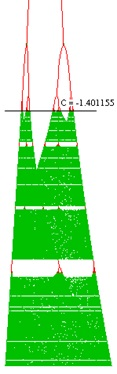
\includegraphics[scale=1]{fx12}
	\caption{De functie $y=x^2+c$ met $c=-1,401155\ldots$.}
	\label{fig:fx12}
\end{figure}
Om terugkomen op de groene waas of beter gezegd de Feigenbaum Fractal, Fig. \ref{fig:fx12}. De boom is in dit figuur uitvergroot en zonder stam (de parabool) weergegeven. In het figuur is te zien dat het gebied waar periodeverdubbeling optreedt eindigt bij een waarde van $c = -1,401155\ldots$ 
Als de c nog negatiever wordt, dan zijn er nog steeds gebieden met x-waardes die worden aangetrokken, maar er ontstaat geen herhalend patroon. De aantrekker is een vreemde aantrekker geworden. De iteraties die daarna komen leveren chaos op. In dit groene chaosgebied zijn nog wel kleine stukjes regelmaat te zien die vervolgens weer overlopen tot chaos. Met het groene vlak is duidelijk te zien dat we niet kunnen voorspellen wat er gaat gebeuren, dat noemen we chaos. 
Als we alles even op een rijtje leggen blijk het volgende: 
In het verdubbelingsgebied is alles voorspelbaar. Daar komt een startwaarde van $x$ komt in een cyclus terecht. Wanneer we een andere startwaarde kiezen, is het begin misschien  verschillend, maar ook dan kom je in dezelfde cyclus terecht. In het chaotisch gebied komt een startwaarde van $x$ niet meer in een cyclus terecht, maar springt op chaotische wijze heen en weer.
Bovendien blijkt dat voor andere startwaarden, zelfs als ze vlak in de buurt van de eerste liggen, de iteraties al snel van elkaar gaan verschillen.

\section{Gevoelens voor wiskunde}
Deze gevoeligheid en precieze voor de keuze van de startwaarde is kenmerkend voor alle chaotische systemen. Fig. \ref{fig:fx12} die we nu besproken hebben is slechts een simpel voorbeeld. De chaostheorie die in de zeventiger jaren van de vorige eeuw opkwam, ontdekte dat chaotische systemen overal voorkomen. Een bekend en leuk voorbeeld van een chaotisch systeem zijn de processen rond luchtdruk en temperatuur, die zich in de atmosfeer bevinden en zo dus ook het weer bepalen. De Amerikaanse meteoroloog Lorenz ontdekte in die tijd min of meer bij toeval dat de resultaten van zijn modelberekeningen heel anders werden wanneer hij  zijn invoergegevens gebruikte die een fractie verschillend waren. Deze extreme gevoeligheid voor de startwaarde betekent in de praktijk onvoorspelbaarheid. We kunnen bijvoorbeeld bij het weersysteem super erg ons best doen om de beginwaarden zoals de temperaturen of de luchtdrukken nauwkeurig op te meten. Maar hoe precies het ook is er zal altijd een onzekerheid overblijven. Als de temperatuur bijvoorbeeld een bepaalde dag $0,1\si{\degree}$ verkeerd wordt gemeten, is de afwijking van de weersvoorspelling voor de dag erna al $0,5\si{\degree}$. Na een week kan er dan al een verschil van meer dan $3\si{\degree}$ naast zitten. Een weervoorspelling voor meer dan twee weken is dan niet zinvol meer. Tegenwoordig worden weersvoorspellingen gedaan door het oplossen van een aantal gekoppelde differentiaalvergelijkingen. Van deze differentiaalvergelijkingen zijn meestal geen exacte oplossingen bekend, maar een numerieke doorberekening kan natuurlijk wel worden gedaan met behulp van veel computerwerk. In de praktijk betekent dit dat er met de weergegevens van een bepaalde dag, die van de dag erna kunnen worden berekend. Het blijkt dat gekoppelde differentiaalvergelijkingen instabiel kunnen zijn. Dat betekend dat er een vorm van chaos in voor komt. Hier geldt ook dat kleine verschillen in beginwaarden veroorzaakt door bijvoorbeeld afrondingsfouten. Een enorme impact hebben in het eindresultaat van de berekening.

\section{De Chaostheorie}
De Chaostheorie is een populair wetenschappelijke benaming voor de theorie van de dynamische systemen. Anders dan de benaming waarmee mijn moeder de toestand van mijn slaapkamer thuis doorgaans beschrijft, wordt hier een technisch wiskundige betekenis bedoeld. Of wel: het onderzoek naar omstandigheden waarbij een deterministische chaos optreedt en welke eigenschappen die chaos heeft. Met een deterministische chaos wordt bedoeld dat de schijnbare wanorde toch exact bepaald is en geordend tot stand komt volgens een algoritme bijvoorbeeld een differentiaalvergelijking of een recursieve berekening. Hiermee kan de stabiliteit en betrouwbaarheid van systemen worden gecontroleerd.
\begin{enumerate}
\item de complexiteit van het systeem
\item de verscheidenheid van de factoren die veranderingen in die systemen veroorzaakten 
\end{enumerate}
\begin{figure}[h]
	\centering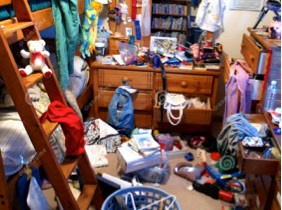
\includegraphics[scale=1]{chaos}
	\caption{Herkenbare chaos.}
	\label{fig:chaos}
\end{figure}
Met de ontwikkeling van de systeemtheorie werd het duidelijk dat dit niet zo is. Zelfs eenvoudige systemen waarin de onderdelen op een niet-lineaire manier beïnvloeden, kunnen het begrip "deterministische chaos" vertonen. Dit kan alleen met behulp van computermodellen worden aangetoond. Het blijkt namelijk dat een zeer kleine verandering in de beginwaarden van een systeem binnen een eindige tijd tot extreem grote veranderingen in de eindwaarde kan zorgen. Een beroemde anekdote is die van de vlinder en de orkaan ook wel bekend als het butterfly effect. Deze is meer bedoeld als verduidelijking van de chaostheorie dan dat deze praktische toepasbaarheid.

\section{De vlinder en de orkaan}
Om even een uitstapje te maken van de moeilijke wiskunde is hier een kleine anekdote die te maken heeft met een van de vele chaostheorieën: the butterfly effect.
De meteoroloog Edward Lorenz introduceerde in 1960 de term The Butterfly Effect. In de anekdote wordt dan gesteld dat een enkele vleugelbeweging van een vlinder in het Amazonegebied voor het verschil kan zorgen voor de weersvoorspelling van of een zonovergoten dag of een hevige storm in Europa: het Butterfly Effect. Hoewel een systeem dus deterministisch kan zijn, wat betekent dat een toekomstige toestand volledig wordt bepaald door de initiële toestand, zonder dat er toeval elementen aan te pas komen, zijn deze systemen dus toch niet voorspelbaar. Deze eigenschap wordt de “deterministische chaos” of kortweg chaos genoemd.
\begin{figure}[h]
	\centering\includegraphics[scale=1]{bradbury}
	\caption{A sound of Thunder, door Bradbury.}
	\label{fig:bradbury}
\end{figure}
Leuke associatie is het feit dat in 4V op het Griftland College één van de short stories in TW2 bij het vak Engels gaat over het Butterfly effect. Dit verhaal heette: Sound of Thunder, geschreven door Ray Bradbury:  "In het jaar 2055 heeft de mens de technologie voor tijdreizen ontwikkeld. Er worden nu onder andere safari’s georganiseerd voor jagers die graag eens op dinosauriërs willen jagen. Er zijn echter wel enkele veiligheidsregels van kracht die moeten voorkomen dat het verleden per ongeluk wordt veranderd; de jagers mogen alleen dieren doden die anders ook rond die tijd gestorven zouden zijn, moeten te allen tijde op een speciaal aangegeven pad blijven, mogen alleen goedgekeurde dieren (zonder toekomst) schieten en mogen niks mee terugnemen.\\
Een jager genaamd Eckels gaat op zo’n safari, samen met de gids Travis, diens assistent Lesperance, en twee medejagers; Billings en Kramer. Vlak voor hun vertrek naar het verleden wordt onthuld dat Keith de presidentsverkiezingen heeft gewonnen van de fascistische kandidaat Deutscher.\\
Wanneer Eckels een Tyrannosaurus ziet, raakt hij in paniek en zet per ongeluk een stap buiten het pad. Terug in het heden blijkt hij bij zijn misstap een vlinder te hebben verpletterd. Dit heeft vergaande gevolgen voor de loop van de tijdlijn, die sterk begint te veranderen. Het begint met subtiele veranderingen zoals Engelse woorden die opeens anders worden uitgesproken (in 1960 vertaald tot N.V. Teit Sefarie), maar gaat steeds verder. Zo blijkt Deutscher opeens de verkiezingen te hebben gewonnen in plaats van Keith. Eckels smeekt Travis terug te mogen naar het verleden in de hoop zijn fout recht te zetten, maar in plaats daarvan richt Travis zijn geweer op hem. Het laatste wat Eckels hoort is “het geluid van gedonder”.

Aan dit verhaal is duidelijk te zien wat voor effect een kleine verandering kan hebben in een chaos.

\section{Fractals in fractals}
We zijn dan eindelijk aangekomen bij het onderdeel waar we gaan kijken wat een fractal eigenlijk is.
Fractals zijn meetkundige figuren met als kenmerk dat alle onderdelen nagenoeg dezelfde meetkundige vormen hebben als het origineel maar dan op steeds kleinere schaal. Dat wilt dus zeggen; als je een fractal zou vergroten met een vergrootglas krijg je steeds weer precies hetzelfde plaatje te zien. Ongeacht de plek waar je kijkt binnen het figuur. Een goed voorbeeld hiervan is de beroemde Mandelbrot Fractal, zie Fig. \ref{fig:mf}.
\begin{figure}[h]
	\centering\includegraphics[scale=1]{mf}
	\caption{Mandelbrot fractal.}
	\label{fig:mf}
\end{figure}
\begin{figure}[h]
	\centering\includegraphics[scale=1]{benoitm}
	\caption{Benoit Mandelbrot.}
	\label{fig:benoitm}
\end{figure}
De Mandelbrot Fractal is vernoemd naar de Poolse wiskundige Benoit Mandelbrot (Fig. \ref{fig:benoitm}) die in de zeventiger jaren van de vorige eeuw onderzoek deed naar fractals. In die tijd werd voor het eerst mogelijk om op de computer graphics te maken. De Mandelbrot Fractal werd in 1991 vermeld in het Guinessbook of Records als "het meest ingewikkelde wiskundige object."

Het zwarte figuur in het midden van Fig. \ref{fig:mf}, ook wel een cardioïde genoemd, is omgeven door een gloeiende rand met in het midden van het figuur aan de buitenkant een soort naald. Het is duidelijk te zien dat op deze naald allemaal kleine cardioïden zitten. Een verdere uitvergroting in dit figuur doet vermoeden dat er nog veel meer hiervan zijn. Dat is ook het geval. Het zijn er zelfs oneindig veel, steeds kleiner en kleiner. Alle punten binnen deze fractal zijn aangrenzende punten. Dit is een bewezen gegeven. Deze fractal is dus samenhangend ofwel gesloten.

Laten we eens wiskundig naar deze fractal kijken. Bij de bewerking van de Mandelbrot Fractal wordt eerst het kwadraat genomen van een complex getal en daarna wordt het oorspronkelijke getal hierbij opgeteld. In de formule-taal ziet dat er als volgt uit:

We gebruiken hiervoor de formule $c=2+0,5i$. We kwadrateren deze formule met behulp van het merkwaardig product
\begin{displaymath}
{\left(x+y\right)}^2=x^2+2xy+y^2.
\end{displaymath}
Dat levert ons het volgende op.
\begin{align*}
{\left(2+0,5i\right)}^2 &= 2^2+2\cdot 2\cdot 0,5i+0,5^2\cdot i^2\\
&= 4+2i+0,25\cdot -1\\
&= 3,75+2i.
\end{align*}
vervolgens wordt hier de 'oude' $c$ bij opgeteld en dan krijg je het volgende.
\begin{displaymath}
(3,75+2i)+(2+0,5i)=5,75+2,5i
\end{displaymath}

Hierboven is de eerste stap van het zogenaamde iteratieproces gemaakt. Je kunt zeggen dat de Mandelbrot Fractal uit oneindig veel van dit soort iteratieprocessen bestaat. Deze iteratieprocessen zijn erg belangrijk voor het maken en begrijpen van fractals. We gaan nu dieper in de ontstaan van fractals in het complexe vlak.    

\section{Complexe fractals}
We zijn eindelijk op het punt gekomen waar we het complexe getal gaan toevoegen aan een Fractal formule. We beginnen weer met de formule $y=x^2+c$. We gebruiken aantrekkingspunten nu niet meer als stukjes van een getallen lijn maar als gedeeltes van het complexe vlak. We beginnen bij Fig. \ref{fig:fx13}. Het grijze vlak geeft hier de aangetrokken getallen aan en het rode sterretje is de aantrekker. In het figuur hiernaast geldt $c=0$ weer. De uitkomst is niet verassend, zoals we al eerder besproken hebben trekken alle reële getallen die tussen -1 en 1 zitten naar het punt 0. In het complexe vlak ziet dat eruit als een cirkelvormig figuur.
\begin{figure}[h]
	\centering\includegraphics[scale=1]{fx13}
	\caption{Fractal in complex vlak met $c=0$.}
	\label{fig:fx13}
\end{figure}
Als we de $c$ gaan veranderen veranderd de vorm van het figuur ook. Als we $c=-0,5$ nemen hadden we gevonden dat alle getallen met als start waarden tussen -1,366 en 1,366 aangetrokken door het punt -0,366. Als we die uitkomsten in een complex vlak zouden zetten. Ziet het er uit als in Fig. \ref{fig:fx14}. De rafelige randen van dit figuur begint al meet te lijken op een fractal maar is nog aardig af te leiden van de cirkelvorming.
Om van die afleiding af te komen hebben we meer dan een aantrekkingspunt nodig. 
\begin{figure}[h]
	\centering\includegraphics[scale=1]{fx14}
	\caption{Fractal in complex vlak met $c=-0,5$.}
	\label{fig:fx14}
\end{figure}
Bij $c=-1$ hadden we gezien dat er twee aantrekkingspunten zijn. De waardes van die aantrekkingspunten zijn 0 en -1. De vorm die hier uitkomt is voor het eerst bedacht zonder computer of rekenmachine door de Franse wiskundige Gaston Julia. En is te zien in Fig. \ref{fig:julfrac}. Dit soort figuren worden daarom ook Julia fractals genoemd. Dit figuur is al minder af te leiden van een cirkel en heeft met de sprietjes iets weg van de Mandelbrot Fractal.
Bij een Julia Fractal zijn de gebieden van het complexe vlak (in de tekening aan geven als grijs vlakdeel) voor gegeven waarde van $c$, bij het irriteren niet naar oneindig gegaan.
\begin{figure}[h]
	\centering\includegraphics[scale=1]{julfrac}
	\caption{Fractal in complex vlak met $c=-1$.}
	\label{fig:julfrac}
\end{figure}

Tot nu toe zijn we bij reële getallen gebleven als het ging om de waarde van $c$. Als we een complex getal nemen voor $c$ bijvoorbeeld: $\Re(c) = - 0.5$ en $\Im(c) = 0.55$ is het fractale karakter waar we uiteindelijk heen willen goed te zien in figuur 13. De vijf dubbele aantrekkers zijn nu zelf ook complex geworden. 
\begin{figure}[h]
	\centering\includegraphics[scale=1]{fx15}
	\caption{Fractal in complex vlak met $\Re(c) = - 0.5$ en $\Im(c) = 0.55$.}
	\label{fig:fx15}
\end{figure}
Om naar een bekende Julia Fractal te kunnen gaan moeten we nog een stapje verder en nemen we $\Re(c) = 0.325$ en $\Im(c) = 0.417$. De negenvoudige aantrekkers hebben een futuristische vorm gecreëerd dat is goed te zien in Fig. \ref{fig:jul2frac}.
\begin{figure}[h]
	\centering\includegraphics[scale=1]{jul2frac}
	\caption{Fractal in complex vlak met $\Re(c) = 0.325$ en $\Im(c) = 0.417$.}
	\label{fig:jul2frac}
\end{figure}

Zoals eerder is gezegd geeft het grijze vlak de aangetrokken punten weer. De rest eromheen itereert naar het oneindige. Met die kennis kleuren we Fig. \ref{fig:jul2frac} in. We tekenen de vorm zelf zwart. Van de gebieden die buiten het figuur liggen bepalen we hoeveel keer het nodig is om te irriteren voordat de uitkomst de zelf gekozen grenswaarde heeft bereikt. Aan de hand van de hoeveelheid iteraties geven we elk punt een kleur. Op die manier hebben we Fig. \ref{fig:jul2frac} ingetekend. De c waarde heeft dezelfde waarde als Fig. \ref{fig:jul2frac}. De kleuren zijn als volgt te verklaren, naarmate het langer duurt voor het itereren de grenswaarde heeft bereikt, hoe lichter de kleur is. Zo kan er veel geknutseld worden met Fractals en kunnen er mooie figuren uitkomen.

We hebben nu gezien hoe een Julia Fractal wordt gemaakt met behulp van complexe getallen. In het begin hebben we gezien dat de reële getallen binnen -2 en 0,25. Dat is een makkelijke en duidelijke richtlijn om een Julia fractal te maken met behulp van reële getallen. Die richtlijn bestaat er ook voor de complexe getallen en is terug te vinden in de Mandelbrot fractal.
Want met de Mandelbrot fractal is er iets heel bijzonders aan de hand. De Mandelbrot Fractal is namelijk een verzameling van alle complexe c-waarden die aantrekkingsgebieden creëren in een Julia Fractal.
\begin{figure}[h]
	\centering\includegraphics[scale=1]{jul2frackleur}
	\caption{Fig. \ref{fig:jul2frac} ingekleurd.}
	\label{fig:jul2frackleur}
\end{figure}

\section{Het nut van een fractal of een fractal van de nuttigheid?}
De fractale wiskunde had een grote populariteit aan het eind van de vorige eeuw. Het leek wel of men overal een fractal in zag. Maar een fractal is net als een cirkel of een vierkant gewoon een wiskundig begrip. Er zijn verschillende toepassingen voor. De meest in het oog springende is de toepassing bij de zogenaamde Chaostheorie. Zonder fractals is het bijna niet mogelijk om chaos te omschrijven.
\begin{figure}[h]
	\centering\includegraphics[scale=1]{blaadje}
	\caption{Een blaadje.}
	\label{fig:blaadje}
\end{figure}
Een andere theorie waar Fractals in worden gebruikt is debifurcatietheorie, die theorie beschrijft hoe het evenwichtsgedrag van een dynamisch systeem verandert onder invloed van externe factoren. Uit deze theorie komt de fractal De Poincaré-afbeelding die ook onder meer gebuikt wordt bij de chaostheorie. 
Fractals worden ook gebruikt bij het karateriseren van kleine of ruwe structuren, bijvoorbeeld blaadjes van varens met een ruwe achterkant of de takstructuur van een boom. Misschien wel de meest actuele toepassing van fractals is het voorspellen van gebeurtenissen. Zoals in de inleiding staat wordt het ontstaan van het heelal aan de hand van fractals voorspeld, maar ook het gedrag van de beurs wordt aan de hand van een fractal voorspeld.
\begin{figure}[h]
	\centering\includegraphics[scale=1]{superfrac}
	\caption{De wonderschone fractal.}
	\label{fig:superfrac}
\end{figure} 
Een leuk voorbeeld over voorspellen is bij het boren naar olie. Bij het boren naar olie gaat de boor waar mee gegraven wordt opeens heftig trillen en gaat kapot, zonder een concrete aanleiding. De trillingen lijken op een fractal waarmee men vervolgens door te modeleren een simulatie van het boorproces mee simuleert en zo de oorzaak zoeken van de trillingen, zodat de boor niet opnieuw stuk gaat.
De schoonheid van fractals mag zeker niet worden vergeten en is ook een van de redenen waarom het zo populair is geworden.

%----------------------------------------------------------------------------------------
%	PART 3
%----------------------------------------------------------------------------------------

\part{Deel Drie}

%----------------------------------------------------------------------------------------
%	CHAPTER 6
%----------------------------------------------------------------------------------------

\chapter{Conclusie}
We hebben heel wat gezien over complexe getallen. We wat ze zijn, waar ze vandaan komen, hoe je ze gebruikt, in welke gebieden ze gebruikt worden. We hebben zelfs drie vrij specifieke toepassingen tot in detail behandeld om te kijken of er een relatie is tussen de verschillende gebruiken van complexe getallen.
Dat was dan ook onze onderzoeksvraag. We hadden verwacht dat complexe getallen gebruikt worden om problemen op te lossen bij het berekenen van bepaalde waarden die niet via de reële getallen te berekenen zijn. Zijn we het nog steeds eens met deze veronderstelling?

\section{Verschillende toepassingen}
We hebben gekeken naar verschillende toepassingen. Laten we naar elke individuele toepassing kijken.

\subsection{Signaalverwerking}
We hebben gezien dat bij signaalverwerking één ingrediënt niet kan ontbreken: de fouriertransformatie. In het kort kan je zeggen dat deze transformatie is uitgevonden om data van het tijd- naar het frequentiedomein te verplaatsen om zo de periodieke natuurlijkheid van de gegevens te bekijken. Er zijn continue vergelijkingen die van een continu signaal de transformatie kunnen berekenen. De continue (inverse) fouriertransformatie. Deze formules zijn niet geschikt voor enkele datapunten. Hiervoor is het discrete fouriertransformatiepaar nodig. Vervolgens hebben we met deze gerekend en onze eigen getransformeerde gemaakt.
De basis voor de signaalverwerking is gelegd. Maar waar wordt het nou precies in gebruikt? Het blijkt dat het gebruikt wordt in de muziek. Bijvoorbeeld om muziek te herkennen met een app: Shazam. Ook wordt het gebruikt om geluidsbestanden te comprimeren of om bepaalde frequenties weg te filteren. Zelfs in de ruimte wordt Fouriers trucje toegepast. Misschien vliegt er nu wel een apparaat rond die uitgerust is met Digital Signal Processing.
Waarom dan complexe getallen? Kan het niet anders? Ja het kan anders. Kijk even snel naar de volgende vergelijking. Deze hebben we expres niet laten zien. Onderstaande hoeft ook niet begrepen te worden.
\begin{displaymath}
\hat{f}\sim\left(\frac{1}{\pi}\int_{-\infty}^\infty\cos{(sx)}\int_{-\infty}^\infty f(y)\cos{(sy)}\,dy\right)+\left(\frac{1}{\pi}\int_{-\infty}^\infty\sin{(sx)}\int_{-\infty}^\infty f(y)\sin{(sy)}\,dy\right)
\end{displaymath}
Deze vergelijking heeft twee termen, dus twee transformaties. De cosinustransformatie en de sinustransformatie. Bij elkaar zijn ze de complete transformatie. Het is natuurlijk veel beter om een berekening sneller uit te kunnen voeren en daarom is er een transformatie bedacht die in één keer berekend kan worden. De fouriertransformatie mag versimpeld worden door gebruik te maken van de formule van Euler \cite{jo}. Complexe getallen zijn daar uitermate geschikt voor. Complexe getallen versimpelen de transformatie.

\subsection{Kwantum}
Bij het kijken naar de toepassing van complexe getallen in de kwantum mechanica en specifiek in de Schrödingervergelijking, kwamen we er achter dat het imaginaire getal gebruikt werd bij berekeningen die als het ware dienden als kansberekeningen. Rekening houdend met de onzekere voortbeweging van kleine deeltjes wordt de Schrödingervergelijking gebruikt om de meest waarschijnlijke plaats en beweging te berekenen. 
In zowel de tijdsafhankelijke als de tijdsonafhankelijke Schrödingervergelijkingen wordt een Hamiltoniaan gebruikt, een korte formule die standaard een imaginair getal in de berekening heeft. Zonder het imaginaire getal zou de Hamiltoniaan een positieve waarde geven, wat de uitkomsten van de Schrödingervergelijking drastisch zou veranderen. Verder gebruikt de tijdsafhankelijke Schrödingervergelijk een imaginair getal in de hoofdformule, waardoor de hieruit gekregen grafiek enkel en alleen in een complex assenstelsel getekend kan worden.
Hieruit wordt duidelijk dat de Schrödingervergelijking, een formule die de basis voor de kwantummechanica vormt, niet mogelijk zou zijn geweest zonder de toepassing van complexe getallen. Complexe getallen vormen dus een essentieel onderdeel van deze natuurkundige kansberekening.

\subsection{Fractals}
We hebben gekeken hoe een fractal is opgebouwd is uit chaos en reële aantrekkingspunten maar ook complexe aantrekkingspunten. De oneindige vormen die kunnen worden gemaakt door middel van een fractal is mede te danken aan het toevoegen van het complexe getal in de formule van een fractal en de vele mogelijkheden van toepassingen waar fractals worden gebruikt om te zoeken naar een oplossingen.

We hebben stap voor stap gezien hoe het itereren van formules een heel belangrijke stap is voor het maken van fractals. De grenswaardes voor de aantrekkingspunten van de reële maar ook complexen getallen kunnen van te voren worden bepaald en daarmee is het begrijpen en maken van een fractal een stuk makkelijker. Door iteratie kan er prachtige kunst worden gemaakt van fractals, waar de manier van denken helemaal in eigen hand is.

We hebben ook gezien dat fractals iets met elkaar te maken kunnen hebben. Zoals dat de Mandelbrot fractal wat een verzameling is van alle complexe $c$-waarden die aantrekkingsgebieden creëren in een Julia Fractal.

Fractals komen we overal tegen en wordt op veel verschillende draagvlakken toegepast.

Door het toevoegen van de complexe getallen krijgen fractals veel meer mogelijkheden en kunnen ze meer en vaker worden gebruikt bij de toepassingen van fractals. 

%----------------------------------------------------------------------------------------
%	BIBLIOGRAPHY
%----------------------------------------------------------------------------------------

\chapter*{Bibliografie}
\addcontentsline{toc}{chapter}{\textcolor{ocre}{Bibliografie}}

%------------------------------------------------
\section*{Deel Een}
\addcontentsline{toc}{section}{Deel Een}
\subsection*{Wat zijn complexe getallen}
\addcontentsline{toc}{subsection}{Wat zijn complexe getallen}
\printbibliography[heading=bibempty,keyword=wat_is_het]

\section*{Deel Twee}
\addcontentsline{toc}{section}{Deel Twee}
\subsection*{Signaalanalyse}
\addcontentsline{toc}{subsection}{Signaalanalyse}
\printbibliography[heading=bibempty,keyword=sign]

\subsection*{Schrödingervergelijking}
\addcontentsline{toc}{subsection}{Schrödingervergelijking}
\printbibliography[heading=bibempty,keyword=schr]

\subsection*{Fractals}
\addcontentsline{toc}{subsection}{Fractals}
\printbibliography[heading=bibempty,keyword=frac]

%----------------------------------------------------------------------------------------
%	INDEX
%----------------------------------------------------------------------------------------

%\cleardoublepage
%\phantomsection
%\setlength{\columnsep}{0.75cm}
%\addcontentsline{toc}{chapter}{\textcolor{ocre}{Index}}
%\printindex

%----------------------------------------------------------------------------------------

\end{document}
